% 第二章 群: 初次相遇 --- 中译
% 原书 pp. 41--98 (Aluffi, Algebra: Chapter 0, Chapter II).
% 本文件进度: §\ref{sec:def-group}--§\ref{subsec:group-objects} 全部译完 (2026-08-29), 第二章完.

\chapter{群:初次相遇}
\label{chap:groups1}


% ===== 记号索引 v1 集中埋点 (页码参考原书书页; 首次出现位置待人工校对) =====
% 本章记号条目（7 条）。OCR 已做最佳校正，但部分符号字形与首次
% 出现位置仍待逐条人工复核（页码沿用原书第 699 页 Index of Notation）。
% ===== /记号索引 =====
\index[sym1]{$D_{2n}$@$D_{2n}$}
\index[sym1]{$G * H$@$G * H$}
\index[sym1]{$G/H$@$G/H$}
\index[sym1]{$\GL_n(\R)$@$\GL_n(\R)$}
\index[sym1]{$H \backslash G$@$H \backslash G$}
\index[sym1]{$\Inn(G)$@$\Inn(G)$}
\index[sym1]{$\SL_2(\Z)$@$\SL_2(\Z)$}
\index{qun@群(group)!zitonggou@自同构(automorphism)}在本章中我们引入群%
\index{qun@群(group)}
, 观察到它们构成一个范畴 (称为 $\cate{Grp}$), 并研究这个范畴的``一般''性质: 这个范畴中的单态射与满态射是什么? 对群来说,``等价关系''与``商''的恰当概念是什么? $\cate{Grp}$ 中是否成立``分解定理''? 以及其他类似的问题.

在第三章中, 我们将对环与模建立起类似程度的熟悉. 对 $\cate{Grp}$ 更面向对象的分析 (例如, 著名的Sylow%
\index{xiluo@Sylow(Sylow)}
\index{Abel qun@Abel 群(abelian group)!hanzi@函子(functor)}\index{Abel@Abel!Niels Henrik@Niels Henrik}定理的处理、``合成列'', 或有限 Abel 群的分类) 则推迟到第四章.

\section{群的定义}
\label{sec:def-group}

\subsection{群与群胚}
\label{subsec:groups-groupoids}

\begin{joke}
\label{joke:group}
\index{qun@群(group)!dezhongxin@的中心(center of a)}定义:群是只有一个对象的群胚%
\index{qunpei@群胚(groupoid)}
.
\end{joke}

这其实是一个完全行得通的定义, 因为群胚已经定义过了 (例~I.\ref{ex:groupoids}); 但大多数数学家会觉得以这种方式引入群是滑稽的, 或者他们至少会礼貌地对这样做的教学效果表示怀疑. 为了给自己赎罪, 作者马上就来剖析这个定义, 以说明它到底说了什么. 若 $*$ 是这样一个群胚 $\cate{G}$ 的唯一对象, 则
\[
\Hom_{\cate{G}}(*, *) = \Aut_{\cate{G}}(*)
\]
(因为 $\cate{G}$ 是群胚!), 而这个集合携带了关于 $\cate{G}$ 的全部信息. 称这个集合为 $G$. 那么 (由范畴的定义) $G$ 上有一个结合的运算, 带有恒同 $1_{*}$, 并且 (由群胚的定义, 它说 $\cate{G}$ 中每个态射都是同构) 每个 $g \in G$ 都有逆 $g^{-1} \in G$.

\index{qun@群(group)!leigongshi@类公式(class formula)}这就是群的全部\footnote{从这个视角看, 玩笑~\ref{joke:group} 有点儿不精确: 群不是群胚 $\cate{G}$, 而是 $\cate{G}$ 中同构构成的集合, 配备态射的复合运算.}: 一个集合 $G$, 带有满足几条关键公理的复合律, 即结合性、恒同的存在性, 以及逆的存在性.

\subsection{定义}
\label{subsec:def-group-official}

现在给出正式的定义. 设 $G$ 是一个非空集合, 配备一个二元运算%
\index{eryuanyunsuan@二元运算(binary operation)}
, 即一个``乘法''映射
\[
\bullet : G \times G \rightarrow G.
\]
我们的记号将是
\[
\bullet(g, h) =: g \bullet h
\]
或者当运算的名字可以理解时干脆写 $gh$. 细心的读者可能曾预期我们应当按范畴那一章的风格写 $h \bullet g$, 但这是通行约定所规定的%
\footnote{并非没有例外; 例如 \S\ref{subsec:symmetric-groups} 中讨论的置换群.}%
.

\begin{definition}
\label{def:group}
配备了二元运算 $\bullet$ 的集合 $G$ (简记 $(G, \bullet)$, 或当运算可以理解时简记 $G$) 称为群, 如果
\begin{enumerate}[label=(\roman*)]
	\item 运算 $\bullet$ 是结合的, 即
	\[
	(\forall g, h, k \in G): \quad (g \bullet h) \bullet k = g \bullet (h \bullet k);
	\]
	\item 存在关于 $\bullet$ 的恒同元%
	\index{hengtongyuan@恒同元(identity element)}
	$e_G$, 即
	\[
	(\exists e_G \in G) (\forall g \in G): \quad g \bullet e_G = g = e_G \bullet g;
	\]
	\item $G$ 中每个元素关于 $\bullet$ 有逆, 即
	\[
	(\forall g \in G) (\exists h \in G): \quad g \bullet h = e_G = h \bullet g.
	\]
\end{enumerate}
\end{definition}

\begin{example}
\label{ex:trivial-group}
由于我们显式要求 $G$ 非空, 造一个群的最经济方式是取 $G = \{e\}$ 为单元素集. 此时只有一个函数 $G \times G \to G$, 因此 $G$ 上只有一种可能的二元运算, 由
\[
e \bullet e := e
\]
定义. 三条公理对这个例子平凡地成立, 于是 $\{e\}$ 带有唯一的群结构.

\index{qun@群(group)!shangtongdiao@上同调(cohomology)}它通常被称为平凡群%
\index{pingfanqun@平凡群(trivial group)}
\index{yuan@元(element)!duichenhanshu@对称函数(symmetric functions)}; 严格主义者应当把任何这样的群都称为``一个''平凡群, 因为每个单元素集都会产生一个.
\end{example}

\begin{example}
\label{ex:number-groups}
读者应当仔细验证 (参见习题~\ref{ex:number-sets-groups}) $(\Z, +)$, $(\Q, +)$, $(\R, +)$, $(\CC, +)$, 以及用 $\cdot$ 的若干变体 (例如, $\Z$ 的子集 $\{+1, -1\}$ 配通常乘法) 都给出群的例子. 这些例子本身虽然非常有趣, 但它们在直观层面上并没有真正捕捉到群``究竟是什么'', 因为它们太特殊了. 例如, 所有这些例子都是交换的 (见 \S\ref{subsec:commutative-groups}).
\end{example}

\begin{example}
\label{ex:GLn}
本书的读者很可能已经熟悉一个极其重要的非交换例子, 即 (比如说) 实元素的、可逆的 $n \times n$ 矩阵%
\index{juzhen@矩阵(matrix)}
之群, $n \geq 2$. 在这些早期章节中我们一般会回避这类例子, 因为等到接触线性代数 (从第六章开始) 时, 我们会有充足的机会思考矩阵. 但在那之前我们偶尔也会借一两个矩阵来用. 读者现在应当验证: 实元素的、满足 $ad - bc \neq 0$ 的 $2 \times 2$ 矩阵
\[
\begin{pmatrix} a & b \\ c & d \end{pmatrix}
\]
\index{qun@群(group)!xunhuan@循环(cyclic)}在通常的矩阵乘法下构成一个群:
\[
\begin{pmatrix} a_1 & b_1 \\ c_1 & d_1 \end{pmatrix} \cdot \begin{pmatrix} a_2 & b_2 \\ c_2 & d_2 \end{pmatrix} = \begin{pmatrix} a_1 a_2 + b_1 c_2 & a_1 b_2 + b_1 d_2 \\ c_1 a_2 + d_1 c_2 & c_1 b_2 + d_1 d_2 \end{pmatrix}.
\]
(条件 $ad - bc \neq 0$ 保证矩阵可逆. 它的逆是什么?) 由于比如
\[
\begin{pmatrix} 1 & 1 \\ 0 & 1 \end{pmatrix} \begin{pmatrix} 1 & 0 \\ 1 & 1 \end{pmatrix} = \begin{pmatrix} 2 & 1 \\ 1 & 1 \end{pmatrix} \neq \begin{pmatrix} 1 & 1 \\ 1 & 2 \end{pmatrix} = \begin{pmatrix} 1 & 0 \\ 1 & 1 \end{pmatrix} \begin{pmatrix} 1 & 1 \\ 0 & 1 \end{pmatrix},
\]
\index{qun@群(group)!youshengchengyuanyuguanximiaoshu@由生成元与关系描述(described by generators and relations)!ermianti@二面体(dihedral)}这个群确实不是交换的.

实元素的、可逆的 $n \times n$ 矩阵之群记作 $\GL_n(\R)$.\index[sym1]{21@$\GL_n(\R)$}

我们将在 \S\ref{sec:examples-groups} 中遇到更有代表性的例子.
\end{example}

\subsection{基本性质}
\label{subsec:basic-properties-group}

从``群胚''的观点看, 恒同元 $e_G$ 应记作 $1_{*}$. 在记号中省去 $G$ (当群已在上下文中明确时) 并用 $1$ 或 $0$ 等不同符号而非 $e$ 来表示这个元素, 都很常见, 视语境而定. 无论如何, 对给定的群 $G$, 这个元素是唯一的. 也就是说, $G$ 中没有别的元素能充当恒同元:

\begin{proposition}
\label{prop:identity-unique}
若 $h \in G$ 是 $G$ 的恒同元, 则 $h = e_G$.
\end{proposition}

顺便说, 这使得群成为例~I.\ref{ex:pointed-sets} 意义下的带基点的集合: 每个群都有一个良定义的特定元素.

\begin{proof}
先用 $e_G$ 是恒同元、再用 $h$ 是恒同元这一事实, 得到%
\footnote{如前所预告, 由于眼下只考虑一个运算, 我们可以省去运算的符号 $\bullet$; 将来我们会不加警告地这样做.}%
\[
h = e_G h = e_G.
\]
(有趣的是, 这个论证只用到 $e_G$ 是``左''恒同元而 $h$ 是``右''恒同元.)
\end{proof}

\begin{proposition}
\label{prop:inverse-unique-group}
逆也是唯一的: 若 $h_1, h_2$ 都是 $g$ 在 $G$ 中的逆, 则 $h_1 = h_2$.
\end{proposition}

\begin{proof}
这其实可以由命题~I.\ref{prop:inverse-unique} 得到 (把 $G$ 看作只有一个对象的群胚的同构之群). 读者应当用同样的技巧构造一个独立的证明, 但小心地把任何对态射的提及都隐藏起来.
\end{proof}

命题~\ref{prop:inverse-unique-group} 授权我们给 $g$ 的逆起个名字: 它通常%
\footnote{但请注意 \S\ref{subsec:commutative-groups} 中讨论的``Abel''情形.}%
记作 $g^{-1}$.

\index{qun@群(group)!duiou@对偶(dual)}还有一项记号上的事项需要交代. 群的定义只涉及两个元素的``乘积''; 在乘一串元素时, 原则上可以选择执行乘法的次序. 例如,
\[
(g_1 \bullet g_2) \bullet g_3
\]
表示: 把运算 $\bullet$ 作用于 $g_1$ 与 $g_2$, 再把 $\bullet$ 作用于该运算的结果与 $g_3$; 而
\[
g_1 \bullet (g_2 \bullet g_3)
\]
表示: 把 $\bullet$ 作用于 $g_2$ 与 $g_3$, 再把它作用于 $g_1$ 与该运算的结果.

结合性恰好告诉我们: 对三个元素执行运算的结果不依赖于执行的方式. 记住这一点, 我们就有资格写
\[
g_1 \bullet g_2 \bullet g_3;
\]
由结合性, 这个表达式没有歧义. 四个或更多元素又如何呢? 读者应当已在习题~I.\ref{ex:associativity-n} 中验证过: 对任意多个元素的一切加括号方式都导致同一个结果. 于是我们也有资格写诸如
\[
g_1 \bullet g_2 \bullet g_3 \bullet \dots \bullet g_{17};
\]
的式子, 这同样没有歧义. 然而读者应当记住, 元素列出的次序当然是重要的: 一般地,
\[
g_1 \bullet g_2 \bullet g_3 \bullet \dots \bullet g_{17} \neq g_2 \bullet g_1 \bullet g_3 \bullet \dots \bullet g_{17}.
\]
当然, 若所有 $g_i$ 都相同, 则无需如此小心; 这时可以使用惯用的``幂''记号%
\footnote{在 Abel 情形, 人们使用``倍数''; 参见 \S\ref{subsec:commutative-groups}.}%
: $g^0 = e_G$, 而对正整数 $n$
\[
g^n = \underbrace{g \cdot \ldots \cdot g}_{n \text{ 次}}, \qquad g^{-n} = \underbrace{g^{-1} \cdot \ldots \cdot g^{-1}}_{n \text{ 次}}.\]\erratumfootnote{根据官方勘误, 明确写出群运算点乘记号.}
容易验证, 于是对 $\forall g \in G$ 与 $\forall m, n \in \Z$ 有
\[
g^{m+n} = g^m g^n.
\]

\subsection{消去}
\index{xiaoqu@消去(cancellation)!zaizhenghuanzhongchengli@在整环中成立(holds in integral domains)}\index{xiaoqu@消去(cancellation)}\label{subsec:cancellation}

群中成立``消去律''. 也就是说,

\begin{proposition}
\label{prop:cancellation}
设 $G$ 是一个群. 则 $\forall a, g, h \in G$
\[
ga = ha \implies g = h, \qquad ag = ah \implies g = h.
\]
\end{proposition}

\begin{proof}
两个断言的证明都是在 (相应的一侧) 乘以 $a^{-1}$ 并应用结合性. 例如,
\[
ga = ha \implies (ga)a^{-1} = (ha)a^{-1} \implies g(aa^{-1}) = h(aa^{-1}) \implies ge_G = he_G \implies g = h.
\]
另一蕴含关系的证明遵循相同的模式.
\end{proof}

不满足消去律、因而不能定义群的运算的例子比比皆是. 例如, 通常的乘法并不能使实数集 $\R$ 成为群: 的确, $0$``不可消去'', 因为即使 $1 \neq 2$ 也有 $1 \cdot 0 = 2 \cdot 0$. 当然, 这里的问题在于 $0$ 在 $\R$ 中关于乘法没有逆. 碰巧, 这是这个例子唯一的问题: 通常的乘法确实使
\[
\R^{*} := \R \setminus \{0\}
\]
\index{qun@群(group)!youxianshengcheng@有限生成(finitely generated)}成为一个群, 读者应当立即自行验证.

\subsection{交换群}
\label{subsec:commutative-groups}

群的定义中不出现的一条公理是交换性: 我们说运算 $\bullet$ 是``交换的'', 如果
\[
(\text{iv})\ (\forall g, h \in G): \quad g \bullet h = h \bullet g.
\]
我们说两个元素 $g$, $h$ ``交换'', 如果 $gh = hg$. 于是, 在交换群中任意两个元素都交换.

``交换群''是重要的对象: 它们在若干语境中自然出现, 尤其是作为``环 $\Z$ 上的模'' (关于这一点, 我们在第三章及以后会大谈特谈). 当它们如此出现时, 通常被称为 Abel 群%
\index{Abelqun@Abel 群(abelian group)}
.

处理 Abel 群时所用的记号与群的标准记号略有不同. 这是为了强调``$\Z$-模结构'', 并且当一个 Abel 群与其他运算共存时会有帮助---这种情形我们将会经常遇到.

于是, Abel 群 $A$ 中的运算按惯例记作 $+$ 并称为``加法''; 恒同元此时称为 $0_A$; 元素 $a \in A$ 的逆记作 $-a$ (或许应当称之为``相反数''?). ``幂''记号当然被``倍数''取代: $0a = 0$, 而对正整数 $n$
\[
na = \underbrace{a + \cdots + a}_{n \text{ 次}}, \qquad (-n)a = \underbrace{(-a) + \cdots + (-a)}_{n \text{ 次}}.\]\erratumfootnote{根据官方勘误, 第二个等式右侧求和中的加号在原书中漏印, 此处予以补正.}
读者应当记住, 在现阶段``$na$''是一个记号, 而不是把二元运算作用于 $A$ 的两个元素 $n$, $a$ 的结果. 的确, $n \in \Z$ 很可能在任何合理的意义下都不是 $A$ 的元素. 而且, 尽管``消去律''在群中成立, 却完全可能出现 $na = ma$ 而 $n \neq m$ 的情形.

``Abel''这一定语以及 $0_A$, $-a$ 等记号, 主要用于在某些标准情形中出现的交换群: 例如, 环、模、向量空间的概念都是通过适当地充实一个交换群来定义的, 出于记号上的方便, 这个交换群随后被提升为``Abel''的.

也有一些交换群自然出现却不触发``Abel''记号的情形. 例如, \S\ref{subsec:cancellation} 末尾提到的群 $(\R^{*}, \cdot)$ 是交换的, 但其运算用 $\cdot$ 表示 (如果写出来的话), 其恒同元写作 $1$. 决定记号的往往是历史而非逻辑.

\subsection{阶}
\label{subsec:order}

\begin{definition}
\index{yuan@元(element)!yunsuan@运算(operation)}\index{yuan@元(element)!yinzi@因子(divisor)}\index{yuan@元(element)!Abel fanchouduixiangde@Abel 范畴对象的(of an object of an abelian category)!chudeng@初等(elementary)}\index{yuan@元(element)}\label{def:order-element}
群 $G$ 的元素 $g$ 称为具有有限阶%
\index{jie@阶(order)}
, 如果 $g^n = e$ 对某个正整数 $n$ 成立%
\footnote{当然, 在 Abel 群中我们会把这条要求写成 $ng = 0$.}%
. 此时, 阶 $|g|$ 是使 $g^n = e$ 的最小正整数 $n$. 若 $g$ 没有有限阶, 则记 $|g| = \infty$.
\end{definition}

按定义, 若 $g^n = e$ 对某个正整数 $n$ 成立, 则 $|g| \leq n$. 可以说得更精确:

\begin{lemma}
\label{lem:order-divides}
若 $g^n = e$ 对某个正整数 $n$ 成立, 则 $|g|$ 整除 $n$.
\end{lemma}

\begin{proof}
如前所观察, 由阶的定义有 $n \geq |g|$, 即 $n - |g| \geq 0$. 于是必定存在%
\footnote{纯粹主义者可能会反对说, 我们在这里偷偷使用了关于 $\Z$ 的相当深入的信息, 即``带余除法'', 因而本质上是 $\Z$ 为 Euclid 整环这一事实! 这些内容只有等到第五章才能得到公正的处理. 我们不妨坦率地承认: 是的, 我们确实假定读者已经对整数的加法与乘法运算非常熟悉. 真是惭愧!}%
正整数 $m$ 使得
\[
r = n - |g| \cdot m \geq 0 \quad \text{并且} \quad n - |g| \cdot (m+1) < 0,
\]
即 $r < |g|$. 注意
\[
g^r = g^{n - |g| \cdot m} = g^n \cdot (g^{|g|})^{-m} = e \cdot e^{-m} = e.
\]
由阶的定义, $|g|$ 是使 $g^{|g|} = e$ 的最小正整数. 由于 $r$ 小于 $|g|$ 且 $g^r = e$, $r$ 不可能是正的; 故必然 $r = 0$. 这就是说
\[
0 = n - |g| \cdot m,
\]
即 $n = |g| \cdot m$, 证明 $n$ 的确如所断言是 $|g|$ 的整数倍.
\end{proof}

这个引理有如下直接而有用的推论, 我们鼓励读者把它牢牢记住:

\begin{corollary}
\label{cor:order-multiple}
设 $g$ 是有限阶元素, $N \in \Z$. 则
\[
g^N = e \iff N \text{ 是 } |g| \text{ 的倍数}.
\]
\end{corollary}

\begin{definition}
\label{def:order-group}
若 $G$ 作为集合是有限的, 其阶%
\index{jie2@阶(order)}
$|G|$ 就是它的元素个数; 若 $G$ 无限, 记 $|G| = \infty$.
\end{definition}

消去律蕴含: 对所有 $g \in G$ 有 $|g| \leq |G|$. 的确, 当 $|G| = \infty$ 时空洞地成立; 若 $G$ 有限, 考虑 $g$ 的 $|G| + 1$ 个幂
\[
g^0 = e, \quad g, \quad g^2, \quad g^3, \quad \ldots, \quad g^{|G|}.
\]
它们不可能两两不同; 于是
\[
(\exists i, j) \quad 0 \leq i < j \leq |G| \quad \text{使得} \quad g^i = g^j.
\]
由消去律 (即在右侧乘以 $g^{-i}$)
\[
g^{j-i} = e,
\]
这表明 $|g| \leq (j - i) \leq |G|$.

关于群的阶与其元素的阶之间的关系, 我们很快就能叙述一个精确得多的命题: 若 $g \in G$ 且 $|G|$ 有限, 则 $g$ 的阶整除 $G$ 的阶. 这将是 Lagrange 定理的直接推论; 参见例~\ref{ex:lagrange-order}.

关于阶的另一条一般性评注是: 阶相对于群的运算的行为并非总是可以预料的: 完全可能 $g$, $h$ 在群 $G$ 中有有限阶, 然而 $|gh| = \infty$, 或者 $|gh| = $ 你最喜欢的正整数: 若不信, 请演算习题~\ref{ex:order-gh-infinity} 与习题~\ref{ex:order-gh-n}.

另一方面, 若 $g$ 与 $h$ 交换, 情形就更有约束. 在 $g = h$ 的极端情形, 容易得到一个非常精确的陈述:

\begin{proposition}
\label{prop:order-power}
设 $g \in G$ 是有限阶元素. 则 $g^m$ 有有限阶 $\forall m \geq 0$, 而且事实上%
\footnote{记号 $\lcm$ 代表``最小公倍数''. 我们还假定读者熟悉 $\gcd$ 与 $\lcm$ 的简单性质.}%
\[
|g^m| = \frac{\lcm(m, |g|)}{m} = \frac{|g|}{\gcd(m, |g|)}.
\]
\end{proposition}

\begin{proof}
两个数 $\frac{\lcm(m, |g|)}{m}$ 与 $\frac{|g|}{\gcd(m, |g|)}$ 的相等由 $\gcd$ 与 $\lcm$ 的初等性质得到: 对一切 $a$ 与 $b$ 有 $\lcm(a,b) = ab/\gcd(a,b)$. 所以我们只需证明 $|g^m| = \frac{\lcm(m, |g|)}{m}$.

$g^m$ 的阶是使
\[
g^{md} = e
\]
的最小正数 $d$, 也就是说 (由推论~\ref{cor:order-multiple}) 使 $md$ 是 $|g|$ 的倍数的最小正数 $d$. 换言之, $m|g^m|$ 是 $m$ 的倍数中同时也是 $|g|$ 的倍数的最小者:
\[
m|g^m| = \lcm(m, |g|).
\]
所陈述的公式随之立得.
\end{proof}

一般地, 对交换的元素,

\begin{proposition}
\label{prop:order-product}
若 $gh = hg$, 则 $|gh|$ 整除 $\lcm(|g|, |h|)$.
\end{proposition}

\begin{proof}
设 $|g| = m$, $|h| = n$. 若 $N$ 是 $m$ 与 $n$ 的任一公倍数, 则由推论~\ref{cor:order-multiple} 有 $g^N = h^N = e$. 由于 $g$ 与 $h$ 交换,
\[
(gh)^N = \underbrace{(gh)(gh) \cdots (gh)}_{N \text{ 次}} = \underbrace{gg \cdots g}_{N \text{ 次}} \cdot \underbrace{hh \cdots h}_{N \text{ 次}} = g^N h^N = e.
\]
由于这对 $m$ 与 $n$ 的每个公倍数 $N$ 都成立, 特别地
\[
(gh)^{\lcm(m,n)} = e.
\]
断言随即由引理~\ref{lem:order-divides} 得到.
\end{proof}

一般说来, 即使 $g$ 与 $h$ 交换, 关于 $|gh|$ 也说不出更多了 (习题~\ref{ex:order-not-lcm}). 但重要特殊情形见习题~\ref{ex:order-coprime}.

\subsection*{习题}
\phantomsection
\addcontentsline{toc}{subsection}{习题}

\begin{prob}
\label{ex:group-as-groupoid}
$\triangleright$ 仔细证明: 每个群都是某个群胚中某个对象的自同构群\erratumfootnote{根据官方勘误, 原书原为``某个群胚的同构之群'', 修正为``某个群胚中某个对象的自同构群''.}. 特别地, 每个群都是某个范畴中某个对象的自同构群. [\S\ref{subsec:symmetric-groups}]
\end{prob}

\begin{prob}
\label{ex:number-sets-groups}
$\triangleright$ 考虑例~1.4\erratumfootnote{根据官方勘误, 此处引用修正为例~1.4 (即 \S\ref{subsec:groups-groupoids}).} 中列出的那些``数集'', 并判定常规运算如 $+$ 与 $\cdot$ 中哪些使它们成为群. 即便答案是否定的 (例如 $(\R, \cdot)$ 不是群), 也请看看这些集合的定义的变体是否产生群 (例如 $(\R^{*}, \cdot)$ 是群; 参见 \S\ref{subsec:cancellation}). [\S\ref{subsec:def-group-official}]
\end{prob}

\begin{prob}
\label{ex:inverse-product}
证明对群 $G$ 的所有元素 $g, h$ 有 $(gh)^{-1} = h^{-1} g^{-1}$.
\end{prob}

\begin{prob}
\label{ex:square-identity}
设群 $G$ 的所有元素 $g$ 都满足 $g^2 = e$; 证明 $G$ 是交换的.
\end{prob}

\begin{prob}
\label{ex:multiplication-table}
\index{chengfabiao@乘法表(multiplication table)}群的``乘法表''是汇编所有乘法 $g \bullet h$ 之结果的表格:
\begin{center}
\renewcommand{\arraystretch}{1.2}
$\begin{array}{c|cccc}
\bullet & e & \cdots & h & \cdots \\ \hline
e & e & \cdots & h & \cdots \\
\cdots & \cdots & \cdots & \cdots & \cdots \\
g & g & \cdots & g \bullet h & \cdots \\
\cdots & \cdots & \cdots & \cdots & \cdots
\end{array}$
\end{center}
\index{Venn@Venn!John@John}\index{Venn@Venn!John@John!tubiao@图表(diagram)}(这里 $e$ 是恒同元. 当然, 该表依赖于元素在顶行与最左列中列出的次序.) 证明: 群的乘法表的每一行与每一列都恰好包含群的每个元素一次 (就像数独图表那样!).
\end{prob}

\begin{prob}
\label{ex:small-groups-tables}
$\neg$ 证明: 若 $G$ 恰有 $1$, $2$ 或 $3$ 个元素, 则 $G$ 只有一种可能的乘法表. 分析恰有 $4$ 个元素的群的各种可能乘法表, 并证明: 在相差 $G$ 的元素重排的意义下, 恰有两张不同的表. 用这些表证明所有元素个数 $\leq 4$ 的群都是交换的.

(欢迎你用同样的技术分析 $5$ 个元素的群, 但你很快就会掌握足够多的群论知识, 从而能够避免这类暴力方法.) [\ref{ex:c5-c12}]
\end{prob}

\begin{prob}
\label{ex:corollary-1-11}
证明推论~\ref{cor:order-multiple}.
\end{prob}

\begin{prob}
\label{ex:unique-order-2}
$\neg$ 设 $G$ 是有限交换群, 恰有一个 $2$ 阶元素 $f$. 证明 $\prod_{g \in G} g = f$. [\ref{ex:wilson}]
\end{prob}

\begin{prob}
\label{ex:order-2-parity}
设 $G$ 是 $n$ 阶有限群, $m$ 是 $G$ 中恰好 $2$ 阶的元素 $g \in G$ 的个数. 证明 $n - m$ 是奇数. 由此断言: 若 $n$ 是偶数, 则 $G$ 必然含有 $2$ 阶元素.
\end{prob}

\begin{prob}
\label{ex:order-g-squared}
设 $g$ 的阶是奇数. 关于 $g^2$ 的阶你能说些什么?
\end{prob}

\begin{prob}
\label{ex:order-gh-equals-hg}
证明对群 $G$ 中所有的 $g, h$ 有 $|gh| = |hg|$. (提示: 证明对 $G$ 中所有的 $a, g$ 有 $|aga^{-1}| = |g|$.)
\end{prob}

\begin{prob}
\label{ex:order-gh-infinity}
$\triangleright$ 在可逆 $2 \times 2$ 矩阵之群中, 考虑
\[
g = \begin{pmatrix} 0 & -1 \\ 1 & 0 \end{pmatrix}, \qquad h = \begin{pmatrix} 0 & 1 \\ -1 & -1 \end{pmatrix}.
\]
验证 $|g| = 4$, $|h| = 3$, 且 $|gh| = \infty$. [\S\ref{subsec:order}]
\end{prob}

\begin{prob}
\label{ex:order-not-lcm}
$\triangleright$ 给出一个表明 $|gh|$ 不必等于 $\lcm(|g|, |h|)$ 的例子, 即便 $g$ 与 $h$ 交换. [\S\ref{subsec:order}, \ref{ex:order-coprime}]
\end{prob}

\begin{prob}
\label{ex:order-coprime}
$\triangleright$ 作为习题~\ref{ex:order-not-lcm} 的对照, 证明: 若 $g$ 与 $h$ 交换且 $\gcd(|g|, |h|) = 1$, 则 $|gh| = |g||h|$. (提示: 令 $N = |gh|$; 则 $g^N = (h^{-1})^N$. 关于这个元素你能说些什么?) [\S\ref{subsec:order}, \ref{ex:maximal-order}, \S~IV.\ref{subsec:sylow-applications}]
\end{prob}

\begin{prob}
\label{ex:maximal-order}
$\neg$ 设 $G$ 是交换群, $g \in G$ 是具有最大有限阶的元素, 即: 若 $h \in G$ 有有限阶, 则 $|h| \leq |g|$. 证明: 事实上若 $h$ 在 $G$ 中有有限阶, 则 $|h|$ 整除 $|g|$. (提示: 反证. 若 $|h|$ 有限但不整除 $|g|$, 则存在素整数 $p$ 使 $|g| = p^m r$, $|h| = p^n s$, 其中 $r$, $s$ 与 $p$ 互素且 $m < n$. 用习题~\ref{ex:order-coprime} 计算 $g^{p^m} h^s$ 的阶.) [\S\ref{subsec:symmetric-groups}, \ref{ex:units-cyclic}, IV.\ref{ex:abelian-max-order}]
\end{prob}

\section{群的例子}
\label{sec:examples-groups}

\subsection{置换群}
\label{subsec:symmetric-groups}

在 \S~I.\ref{subsec:isomorphisms} 中我们已经观察到: 每个范畴 $\cate{C}$ 的每个对象 $A$ 都确定一个群, 即 $A$ 的自同构群 $\Aut_{\cate{C}}(A)$. 在某种人为的意义下, 每个群都以这种方式产生是显然的 (参见习题~\ref{ex:group-as-groupoid}); 这一事实在更``有意义''的意义下也为真, 当我们讨论群作用 (\S\ref{sec:group-actions}) 时将变得明显: 特别参见定理~\ref{thm:cayley} 与习题~\ref{ex:aut-gset}.

无论如何, 这一观察为读者提供了一族无穷的、极其重要的例子:

\begin{definition}
\label{def:symmetric-group}
设 $A$ 是一个集合. $A$ 的置换群%
\index{zhihuanqun@置换群(permutation group)}
(或 $A$ 的置换之群) 记作 $S_A$, 即群 $\Aut_{\cate{Set}}(A)$. 集合 $\{1, \ldots, n\}$ 的置换之群记作 $S_n$.
\end{definition}

这个术语很容易解释: 集合 $A$ 的自同构就是 $A$ 到自身的集合同构, 即双射; 施加这样的双射恰恰就是``打乱''$A$ 的元素. 这个运算可视为 $A$ 的一个不改变它 (作为集合) 的变换, 因而是``对称''.

众所周知 $S_A$ 是巨大的: 正如读者在习题~I.\ref{ex:bijections-count} 中验证过的, $|S_n| = n!$. 例如 $|S_{70}| > 10^{100}$, 这比可观测宇宙中基本粒子数目的估计值大得多.

一个可能引起混淆的地方: 各种约定在 $S_A$ 中运算该如何书写的问题上发生冲突. 从``自同构''的观点看, $S_A$ 的元素是函数, 应当按函数来复合; 于是, 若 $f, g \in S_A = \Aut_{\cate{Set}}(A)$, 则 $f$ 与 $g$ 的``乘积''应写作 $g \circ f$, 且作用方式如下:
\[
(\forall p \in A): \quad g \circ f (p) = g(f(p)).
\]
但群论中流行的书写风格会把这个元素写作 $fg$, 表面上颠倒了运算执行的次序.

如果我们采用把函数写在其作用对象之后而非之前的约定---写 $(p)f$ 而非 $f(p)$---一切都会重新归于一致. 但人们无法改变百年积习, 所以我们别无选择, 只能与两种约定共处, 并在每一时刻小心声明我们用的是哪一种.

思考较小的 $n$ 对应的群 $S_n$ 是一项价值无法估量的练习. 当然 $S_1$ 是平凡群; $S_2$ 由两个可能的置换构成:
\[
\left\{ \begin{array}{l} \mathbf{1} \mapsto \mathbf{1} \\ \mathbf{2} \mapsto \mathbf{2} \end{array} \right. \quad \text{和} \quad \left\{ \begin{array}{l} \mathbf{1} \mapsto \mathbf{2} \\ \mathbf{2} \mapsto \mathbf{1} \end{array} \right.
\]
我们可以把它们称为 $e$ (恒同) 与 $f$ (翻转), 其运算为
\[
ee = ff = e, \qquad ef = fe = f.
\]
实践中我们无法给每个置换群的每个不同元素都起新名字, 所以必须发展更灵活的记号. 实际上有若干可能的选择; 眼下, 我们将这样表示元素 $\sigma \in S_n$: 在清单 $1, \ldots, n$ 的下方列出施加 $\sigma$ 的效果, 即排成一个矩阵%
\footnote{这仅仅是一种记号手段---这些矩阵不应与 (比如) 例~\ref{ex:GLn} 中考虑的矩阵相混淆.}%
. 于是 $S_2$ 中的元素 $e$, $f$ 可以记作
\[
e = \begin{pmatrix} 1 & 2 \\ 1 & 2 \end{pmatrix}, \qquad f = \begin{pmatrix} 1 & 2 \\ 2 & 1 \end{pmatrix}.
\]
用同样的记号风格, $S_3$ 由
\[
\left\{ \begin{pmatrix} 1 & 2 & 3 \\ 1 & 2 & 3 \end{pmatrix},\ \begin{pmatrix} 1 & 2 & 3 \\ 2 & 1 & 3 \end{pmatrix},\ \begin{pmatrix} 1 & 2 & 3 \\ 3 & 2 & 1 \end{pmatrix},\ \begin{pmatrix} 1 & 2 & 3 \\ 1 & 3 & 2 \end{pmatrix},\ \begin{pmatrix} 1 & 2 & 3 \\ 3 & 1 & 2 \end{pmatrix},\ \begin{pmatrix} 1 & 2 & 3 \\ 2 & 3 & 1 \end{pmatrix} \right\}
\]
构成.

至于乘法, 我们将采用上面提到的那个明智 (但不太标准) 的约定, 让置换``从右侧''作用: 于是, 比如
\[
\mathbf{1} \begin{pmatrix} 1 & 2 & 3 \\ 2 & 1 & 3 \end{pmatrix} \begin{pmatrix} 1 & 2 & 3 \\ 3 & 1 & 2 \end{pmatrix} = \mathbf{2} \begin{pmatrix} 1 & 2 & 3 \\ 3 & 1 & 2 \end{pmatrix} = \mathbf{1}
\]
类似地
\[
\mathbf{2} \begin{pmatrix} 1 & 2 & 3 \\ 2 & 1 & 3 \end{pmatrix} \begin{pmatrix} 1 & 2 & 3 \\ 3 & 1 & 2 \end{pmatrix} = \mathbf{3}, \qquad \mathbf{3} \begin{pmatrix} 1 & 2 & 3 \\ 2 & 1 & 3 \end{pmatrix} \begin{pmatrix} 1 & 2 & 3 \\ 3 & 1 & 2 \end{pmatrix} = \mathbf{2}.
\]
也就是说,
\[
\begin{pmatrix} 1 & 2 & 3 \\ 2 & 1 & 3 \end{pmatrix} \begin{pmatrix} 1 & 2 & 3 \\ 3 & 1 & 2 \end{pmatrix} = \begin{pmatrix} 1 & 2 & 3 \\ 1 & 3 & 2 \end{pmatrix}
\]
因为等号两侧的置换对 $\mathbf{1}$, $\mathbf{2}$, $\mathbf{3}$ 的作用方式相同. 读者现在应当验证
\[
\begin{pmatrix} 1 & 2 & 3 \\ 3 & 1 & 2 \end{pmatrix} \begin{pmatrix} 1 & 2 & 3 \\ 2 & 1 & 3 \end{pmatrix} = \begin{pmatrix} 1 & 2 & 3 \\ 3 & 2 & 1 \end{pmatrix}.
\]
也就是说, 令
\[
x = \begin{pmatrix} 1 & 2 & 3 \\ 2 & 1 & 3 \end{pmatrix}, \qquad y = \begin{pmatrix} 1 & 2 & 3 \\ 3 & 1 & 2 \end{pmatrix},
\]
则
\[
yx \neq xy,
\]
这表明 $S_3$ 中的运算不满足交换公理. 于是, $S_3$ 是非交换群; 读者会立即意识到, 事实上对所有 $n \geq 3$, $S_n$ 都是非交换的.

虽然交换关系不成立, $S_3$ 中却有其他有趣的关系成立. 例如
\[
x^2 = e, \qquad y^3 = e,
\]
这表明 $S_3$ 含有 $1$ 阶 (恒同元 $e$)、$2$ 阶 (元素 $x$) 与 $3$ 阶 (元素 $y$) 的元素; 参见习题~\ref{ex:order-d-in-sn}. (顺便说, 这表明习题~\ref{ex:maximal-order} 的结论确实需要交换性假设.) 此外
\[
yx = \begin{pmatrix} 1 & 2 & 3 \\ 3 & 2 & 1 \end{pmatrix} = xy^2,
\]
读者可以验证. 利用这些关系, 我们看到: 由 $x$ 与 $y$ 任意搭配而成的乘积 $x^{i_1} y^{i_2} x^{i_3} y^{i_4} \cdots$ 都可以化归为乘积 $x^i y^j$, 其中 $0 \leq i \leq 1$, $0 \leq j \leq 2$, 也就是化归为六个元素
\[
e, \quad y, \quad y^2, \quad x, \quad xy, \quad xy^2
\]
之一; 例如
\[
y^7 x^{13} y^5 = (y^3)^2 y (x^2)^6 x y^3 y^2 = (yx) y^2 = (xy^2) y^2 = x y^3 y = xy.
\]
另一方面, 这六个元素两两不同---这可以用消去律与阶的考虑来检验%
\footnote{当然, 也可以通过显式计算相应的置换来检验, 但我们是在努力说明``这些关系就是我们所需知道的一切''这一事实.}%
. 例如, 若有 $xy^2 = y$, 则由消去律得 $x = y^{-1}$, 而这是不可能的, 因为那些关系告诉我们 $x$ 的阶为 $2$ 而 $y^{-1}$ 的阶为 $3$.

结论是: 上面展示的六个乘积必定就是 $S_3$ 的全部六个元素:
\[
S_3 = \{e, x, y, xy, y^2, xy^2\}.
\]
在这个过程中我们验证了: $S_3$ 也可以描述为由两个元素 $x$ 与 $y$ ``生成''的群, 带有``关系''$x^2 = e$, $y^3 = e$, $yx = xy^2$.

\index{ziqundepeiji@子群的陪集(cosets of a subgroup)}\index{ziqun@子群(subgroup)!chuandi@传递(transitive)!S_n 的@$S_n$ de}\index{ziqun@子群(subgroup)!wendingzi@稳定子(stabilizer)}\index{ziqun@子群(subgroup)!xunhuanqunde@循环群的(of cyclic group)}\index{ziqun@子群(subgroup)!ziyouqunde@自由群的(of a free group)}\index{ziqun@子群(subgroup)!zhengguihuazi@正规化子(normalizer)}\index{ziqun@子群(subgroup)!zhenggui@正规(normal)}\index{ziqun@子群(subgroup)!dezhishu@的指数(index of)}\index{ziqun@子群(subgroup)!youzijishengcheng@由子集生成(generated by a subset)}\index{ziqun@子群(subgroup)!xunhuan@循环(cyclic)}\index{ziqun@子群(subgroup)!depeiji@的陪集(cosets of)}\index{ziqun@子群(subgroup)!huanweizi@换位子(commutator)}\index{ziqun@子群(subgroup)!tezheng@特征(characteristic)}\index{ziqun@子群(subgroup)!zhongxinhuazi@中心化子(centralizer)}\index{ziqun@子群(subgroup)!p-Sylow@p-Sylow}更一般地, 群 $G$ 的子集 $A$``生成''$G$, 如果 $G$ 的每个元素都可以写成 $A$ 的元素与 $A$ 的元素的逆的乘积. 我们将在 \S\ref{subsec:subgroups-generated} 中更正式地处理这个概念, 并在 \S\ref{subsec:presentations} 中处理用生成元与关系描述群的问题.

\subsection{二面体群}
\label{subsec:dihedral-groups}

\index{fanchou@范畴(category)!Ab@Ab!fan@反(opposite)}``对称''是保持某个结构的变换. 当我们懒得严格定义相关的范畴时, 这当然只是谈论自同构的一种松散方式. 作为范畴对象的自同构, 对称自然构成群.

一个可以把这个概念形象化的语境, 是诸如平面上的多边形或空间中的多面体之类的``几何图形''. 相关的范畴可以这样定义: 把对象取为普通平面 $\R^2$ 的子集, 两个子集 $A$, $B$ 之间的态射由平面的那些把 $A$ 映到 $B$ 的子集的``刚体运动'' (如平移、旋转或关于一条直线的反射) 构成. 严格处理这些概念在此时过于离题, 所以我们将像时常所做的那样, 诉诸读者的直观.

\index{qun@群(group)!youxianbiaoxian@有限表现(finitely presented)}从这个视角看, 平面子集的``对称''就是把它映到自身的刚体运动; 它们显然构成群.

\index{qun@群(group)!ziyou@自由(free)}二面体群%
\index{ermiantiqun@二面体群(dihedral group)}
可以定义为正多边形所对应的这些对称群. 把多边形摆放成以原点为中心 (从而排除平移作为可能的对称), 我们看到: 正 $n$ 边形的二面体群由绕原点旋转角度 $2\pi/n$ 的 $n$ 个旋转以及关于过原点与一个顶点或一条边的中点的直线的 $n$ 个反射构成.

于是, 正 $n$ 边形的二面体群由 $2n$ 个元素构成; 我们将%
\footnote{遗憾的是, 这个记号似乎没有普遍的共识: 有些文献把此处记为 $D_{2n}$ 的群记作 $D_n$.}%
把这个群记作 $D_{2n}$.\index[sym1]{12@$D_{2n}$}

同样, 思考这些群 (至少对较小的 $n$) 是绝好的练习. 有一个简单的方式把二面体群与 \S\ref{subsec:symmetric-groups} 的置换群联系起来, 它抓住了一个事实: 正多边形 $P$ 的对称由 $P$ 的顶点的去向决定. 例如, 把等边三角形的顶点按顺时针方向标记为 $\mathbf{1}$, $\mathbf{2}$, $\mathbf{3}$; 那么逆时针旋转角度 $2\pi/3$ 把顶点 $\mathbf{1}$ 送到 $\mathbf{3}$, $\mathbf{3}$ 送到 $\mathbf{2}$, $\mathbf{2}$ 送到 $\mathbf{1}$, 而且没有其他对称这样做.

直观上看, 就是
\begin{center}
\begin{tikzpicture}[scale=0.85, >=Stealth]
	% 等边三角形
	\coordinate (T) at (0,1.9);
	\coordinate (L) at (-1.65,0);
	\coordinate (R) at (1.65,0);
\index{xunhuan@循环(cyclic)!jihao@记号(notation)}\index{xunhuan@循环(cyclic)}	\draw[thick] (T) -- (L) -- (R) -- cycle;
	\node at (0.02,1.45) {$\mathbf{1}$};
	\node at (-0.95,0.35) {$\mathbf{3}$};
	\node at (0.95,0.35) {$\mathbf{2}$};
	% 旋转箭头 (逆时针)
	\draw[->] (0.55,1.95) arc (65:175:1.5);
	\draw[->] (-1.35,-0.45) arc (205:295:1.5);
	\draw[->] (2.05,0.75) arc (25:95:1.35);
\end{tikzpicture}
\end{center}
换言之, 我们可以把等边三角形的逆时针旋转 $2\pi/3$ 对应于置换
\[
\begin{pmatrix} 1 & 2 & 3 \\ 3 & 1 & 2 \end{pmatrix} \in S_3.
\]
这样的标记定义了一个函数
\[
D_6 \rightarrow S_3;
\]
而且这个函数是单射 (因为对称由它诱导的顶点置换决定). 用我们迟早会掌握的更高级的语言, 我们说 $D_6$ (忠实地) 作用在集合 $\{\mathbf{1}, \mathbf{2}, \mathbf{3}\}$ 上.

显然这可以有多种做法 (例如, 我们可以用不同的方式标记顶点). 然而, 任何这样的指派都有这样的性质: $D_{2n}$ 中对称的复合对应于 $S_n$ 中置换的复合; 读者应当对涉及 $D_6 \rightarrow S_3$ 与 $D_8 \rightarrow S_4$ 的若干例子仔细演算这一点.

描述这一情形的简洁方式是: 这些函数是 (群的) 同态 (参见 \S\ref{sec:group-homomorphisms}). 由于 $D_6$ 与 $S_3$ 都有 $6$ 个元素, 且上面给出的函数 $D_6 \rightarrow S_3$ 是单射, 它必然也是满射. 于是存在 $D_6$ 与 $S_3$ 之间的双射同态; 我们说这两个群是同构的 (参见 \S\ref{subsec:iso-groups}). 我们将在接下来几节中非常仔细地研究这些概念.

作为得出同一结论的另一种 (更抽象的) 方式, 把上面考虑的逆时针旋转记为 $y$, 并把关于过等边三角形中心与顶点 $\mathbf{3}$ 的直线的反射记为 $x$:
\begin{center}
\begin{tikzpicture}[scale=0.85, >=Stealth]
	% 等边三角形
	\coordinate (T) at (0,2.8579);
	\coordinate (L) at (-1.65,0);
	\coordinate (R) at (1.65,0);
	\draw[thick] (T) -- (L) -- (R) -- cycle;
	\node at (0.02,2.20) {$\mathbf{1}$};
	\node at (-0.95,0.35) {$\mathbf{3}$};
	\node at (0.95,0.35) {$\mathbf{2}$};
	% 反射轴 (过顶点3与中心的虚线)
	\draw[dashed] (-2.145,-0.2858) -- (2.145,2.1911);
	% 双向弯曲箭头 (表示翻转)
	\draw[->] (2.1,1.75) arc (60:15:1.9);
	\draw[->] (2.62,-0.1) arc (-30:14:1.9);
\end{tikzpicture}
\end{center}
反射两次给出恒同, 旋转三次亦然; 于是
\[
x^2 = e, \qquad y^3 = e.
\]
进而, $yx$ (先逆时针旋转 $2\pi/3$, 再关于那条斜线翻转) 与 $xy^2$ (先翻转, 再顺时针旋转 $2\pi/3$) 是同一个对称. 也就是说,
\[
yx = xy^2.
\]
换言之, 群 $D_6$ 也由两个元素 $x$, $y$ 生成, 满足关系 $x^2 = e$, $y^3 = e$, $yx = xy^2$---与我们在 $S_3$ 中发现的完全一样. 由于 $D_6$ 与 $S_3$ 都有用生成元与关系表述的匹配描述 (即匹配的表现%
\index{biaoxian@表现(presentation)}
; 参见 \S\ref{subsec:presentations}), 它们``当然''同构.

\index{youxianyu@有限域(finite field)}\index{xunhuanqun@循环群(cyclic group)!youxianyudechengfaqun@有限域的乘法群(the multiplicative group of a finite field)}\index{xunhuanqun@循环群(cyclic group)}\subsection{循环群与模算术}
\label{subsec:cyclic-groups}

设 $n$ 是正整数. 考虑 $\Z$ 上由%
\footnote{记号 $n \mid m$ 表示 $n$ 是 $m$ 的因子; 也就是说, $m = nk$ 对某个整数 $k$ 成立.}%
下式定义的等价关系
\[
(\forall a, b \in \Z): \quad a \equiv b \bmod n \iff n \mid (b - a).
\]
它称为模 $n$ 同余%
\index{tongyu@同余(congruence)}
. 对 $n = 2$, 我们已在例~I.\ref{ex:mod-two} 中遇到过这个关系. 很容易验证: 对所有 $n$ 它都是等价关系; 其等价类之集常记作 $\Z_n$, $\Z/(n)$, $\Z/n\Z$ 或 $\mathbb{F}_n$. 我们将选用 $\Z/n\Z$, 因为它未被其他概念所占用%
\footnote{当 $n = p$ 为素数时, $\Z_p$ 是``$p$-进整数''的官方记号, 那是完全不同的概念; 参见习题~VIII.\ref{ex:p-adic}.}%
. 我们用 $[a]_n$ 表示整数 $a$ 模 $n$ 的等价类, 无歧义时简写 $[a]$.

读者应当仔细验证 $\Z/n\Z$ 恰由 $n$ 个元素构成, 即
\[
[0]_n, \quad [1]_n, \quad \ldots, \quad [n-1]_n.
\]
我们可以利用 $\Z$ 上的群结构在 $\Z/n\Z$ 上诱导一个 (Abel) 群结构. 为此, 我们如下定义 $\Z/n\Z$ 上的运算 $+$: 对 $\forall a, b \in \Z$ 规定
\[
[a] + [b] := [a + b].
\]
当然必须检验这个规定是良定义的; 幸运的是这很容易: 下面的小引理就能办成这件事, 因为它表明运算的结果不依赖于为各等价类所选的代表元.

\begin{lemma}
\label{lem:congruence-add}
若 $a \equiv a' \bmod n$ 且 $b \equiv b' \bmod n$, 则
\[
(a + b) \equiv (a' + b') \bmod n.
\]
\end{lemma}

\begin{proof}
由假设 $n \mid (a' - a)$ 且 $n \mid (b' - b)$; 于是存在 $k, \ell \in \Z$ 使
\[
(a' - a) = kn, \qquad (b' - b) = \ell n.
\]
那么
\[
(a' + b') - (a + b) = (a' - a) + (b' - b) = kn + \ell n = (k + \ell) n,
\]
证明 $n$ 整除 $(a' + b') - (a + b)$, 正如所需.
\end{proof}

于是, 我们得到 $\Z/n\Z$ 上的一个二元运算 $+$. 立即可以验证所得到的结构是一个群. 结合性从 $\Z$ 继承而来:
\[
([a] + [b]) + [c] = [a + b] + [c] = [(a+b) + c] = [a + (b+c)] = [a] + [b+c] = [a] + ([b] + [c]);
\]
恒同元 $[0]$ 与``逆''$-[a] = [-a]$ 也是如此.

同样立即可验证: 所得的群 $\Z/n\Z$ 是交换的, 正如 Abel 式的记号所暗示的那样:
\[
[a] + [b] = [a + b] = [b + a] = [b] + [a].
\]
我们相信这些内容对读者并不新鲜; 无论如何, 读者应当仔细验证所有这些断言.

如此得到的 Abel 群连同 $\Z$ 一起, 称为循环群%
\index{xunhuanqun@循环群(cyclic group)}
; 群 $(\Z/n\Z, +)$ 的一个流行替代记号是 $C_n$. 当想用``乘法''而非``加法''记号时特别会采用它; 于是我们可以说, $C_n$ 由一个元素 $x$ 生成, 带有关系 $x^n = e$.

循环群极其重要, 我们会在后面的各节中回到它们. 眼下我们记录这样一个事实: 元素
\[
[1]_n \in \Z/n\Z
\]
生成这个群, 意思是每个其他元素都可以表示为该元素的倍数. 例如, 若 $m \geq 0$ 是整数, 则
\[
[m]_n = [\underbrace{1 + \cdots + 1}_{m \text{ 次}}]_n = \underbrace{[1]_n + \cdots + [1]_n}_{m \text{ 次}} = m \cdot [1]_n.
\]
等价地, 我们可以这样陈述这一事实: $[1]_n$ 在 $\Z/n\Z$ 中的阶为 $n$: 这意味着 $n$ 个倍数 $0 \cdot [1]_n$, $1 \cdot [1]_n$, $\ldots$, $(n-1) \cdot [1]_n$ 必定两两不同, 从而它们必定填满 $\Z/n\Z$.

\begin{proposition}
\label{prop:order-class}
$[m]_n$ 在 $\Z/n\Z$ 中的阶, 当 $n \mid m$ 时为 $1$; 更一般地
\[
|[m]_n| = \frac{n}{\gcd(m, n)}.
\]
\end{proposition}

\begin{proof}
若 $n \mid m$, 则 $[m]_n = [0]_n$. 若 $n$ 不整除 $m$, 再次观察 $[m]_n = m[1]_n$ 并应用命题~\ref{prop:order-power}.
\end{proof}

\begin{remark}
\label{rem:order-divides}
由此可知, $\Z/n\Z$ 中每个元素的阶都整除 $n = |\Z/n\Z|$, 即群的阶. 我们稍后 (例~\ref{ex:lagrange-order}) 会看到, 这是任意有限群中元素之阶的一个一般特征.
\end{remark}

\begin{corollary}
\label{cor:generates}
类 $[m]_n$ 生成 $\Z/n\Z$ 当且仅当 $\gcd(m,n) = 1$.
\end{corollary}

这个简单的结果相当重要. 例如, 若 $n = p$ 是素整数, 它表明群 $\Z/p\Z$ 中每个非零类都生成它. 无论如何, 它使我们能够构造更多有趣群的例子. 读者应当验证 (或回忆; 参见习题~\ref{ex:congruence-multiplication}) 在 $\Z/n\Z$ 上还有一个良定义的乘法, 由
\[
[a]_n \cdot [b]_n := [ab]_n
\]
给出.

这个运算并不能赋予 $\Z/n\Z$ 群结构: 的确, 类 $[0]_n$ 没有乘法逆. 另一方面, 对任意正整数 $n$, 把 $\Z/n\Z$ 中由满足 $\gcd(m,n) = 1$ 的类 $[m]_n$ 组成的子集记作 $(\Z/n\Z)^{*}$:
\[
(\Z/n\Z)^{*} := \{[m]_n \in \Z/n\Z \mid \gcd(m, n) = 1\}.
\]
这个子集显然是良定义的: 若 $m \equiv m' \bmod n$, 则 $\gcd(m,n) = 1 \iff \gcd(m',n) = 1$ (习题~\ref{ex:congruence-gcd}), 所以 $(\Z/n\Z)^{*}$ 中类的定义性质与代表元的选取无关.

\begin{proposition}
\label{prop:units-group}
乘法使 $(\Z/n\Z)^{*}$ 成为一个群.
\end{proposition}

\begin{proof}
$\gcd$ 的简单性质表明: 若 $\gcd(m_1, n) = \gcd(m_2, n) = 1$, 则 $\gcd(m_1 m_2, n) = 1$. (比如, 若一个素整数同时整除 $n$ 与 $m_1 m_2$, 则它必然整除 $m_1$ 或 $m_2$, 于是两个 $\gcd$ 之一就不是 $1$.) 因此, $(\Z/n\Z)^{*}$ 中两个元素的乘积是 $(\Z/n\Z)^{*}$ 的元素, 且 $\cdot$ 确实定义了一个二元运算
\[
(\Z/n\Z)^{*} \times (\Z/n\Z)^{*} \rightarrow (\Z/n\Z)^{*}.
\]
显然这个运算是结合的 (因为乘法在 $\Z$ 中结合); $[1]_n$ 是 $(\Z/n\Z)^{*}$ 的元素且关于乘法是恒同元; 于是我们唯一需要检验的是: $(\Z/n\Z)^{*}$ 中的元素在 $(\Z/n\Z)^{*}$ 中有乘法逆.

这由推论~\ref{cor:generates} 得到. 若 $\gcd(m, n) = 1$, 则 $[m]_n$ 生成加法群 $\Z/n\Z$, 从而 $[m]_n$ 的某个倍数必等于 $[1]_n$:
\[
(\exists a \in \Z): \quad a \cdot [m]_n = [1]_n;
\]
这意味着
\[
[a]_n [m]_n = [1]_n.
\]
因此 $[m]_n$ 在 $\Z/n\Z$ 中确有乘法逆, 即 $[a]_n$. 读者将验证 $\gcd(a,n) = 1$, 从而完成证明.
\end{proof}

例如, $[8]_{15}$ 在 $(\Z/15\Z)^{*}$ 中有乘法逆. 循着证明中给出的论证,
\[
2 \cdot 8 + (-1) \cdot 15 = 1,
\]
从而 $[2]_{15} \cdot [8]_{15} = [1]_{15}$: $[8]_{15}$ 的乘法逆是 $[2]_{15}$.

当 $n = p$ 为正素整数时, 群 $((\Z/p\Z)^{*}, \cdot)$ 的阶为 $p - 1$. 关于这些群, 我们将在后面的各节中多说几句 (参见例~\ref{ex:units-prime}).

\subsection*{习题}
\phantomsection
\addcontentsline{toc}{subsection}{习题}

\begin{prob}
\label{ex:permutation-matrix}
$\neg$ 可以给置换 $\sigma \in S_n$ 配一个 $n \times n$ 矩阵 $M_{\sigma}$: 令其在 $(i, (i)\sigma)$ 处的元素为 $1$\erratumfootnote{根据官方勘误, 原书原为 $(i, \sigma(i))$, 由于本处置换采用右作用记号, 矩阵在 $(i, (i)\sigma)$ 处取值为 $1$.}, 其余元素均为 $0$. 例如, 对应于置换
\[
\sigma = \begin{pmatrix} 1 & 2 & 3 \\ 3 & 1 & 2 \end{pmatrix} \in S_3
\]
的矩阵是
\[
M_{\sigma} = \begin{pmatrix} 0 & 0 & 1 \\ 1 & 0 & 0 \\ 0 & 1 & 0 \end{pmatrix}.
\]
证明: 采用这套记号, 对一切 $\sigma, \tau \in S_n$ 有
\[
M_{\sigma\tau} = M_{\sigma} M_{\tau},
\]
\index{ji@积(product)!ziyou@自由(free)}其中右端的乘积是通常的矩阵乘积. [IV.\ref{ex:sign-determinant}]
\end{prob}

\begin{prob}
\label{ex:order-d-in-sn}
$\triangleright$ 证明: 若 $d \leq n$, 则 $S_n$ 含有 $d$ 阶元素. [\S\ref{subsec:symmetric-groups}]
\end{prob}

\begin{prob}
\label{ex:order-n-in-sn}
对每个正整数 $n$, 在 $S_N$ 中找出一个 $n$ 阶元素.
\end{prob}

\begin{prob}
\label{ex:D8-to-S4}
像 \S\ref{subsec:dihedral-groups} 中对三角形所做的那样, 通过标记正方形的顶点定义一个同态 $D_8 \to S_4$. 列出该同态像中的 $8$ 个置换.
\end{prob}

\begin{prob}
\label{ex:dihedral-presentation}
$\triangleright$ 描述所有二面体群 $D_{2n}$ 的生成元与关系. (提示: 设 $x$ 是关于正 $n$ 边形过中心与一个顶点的直线的反射, $y$ 是逆时针旋转 $2\pi/n$. 群 $D_{2n}$ 将由 $x$ 与 $y$ 生成, 满足三条关系%
\footnote{两条关系是显然的. 要``看到''第三条, 把你的右手举在面前稍远处, 手指指向一个想象中的正五边形的顶点. 把手朝你自己翻转让五边形翻转; 绕视线方向逆时针旋转 $72^{\circ}$; 再把手背离你翻过去; 然后再次逆时针旋转. 这时手回到了初始位置. 这告诉你什么?}%
. 要看出这些关系确实决定 $D_{2n}$, 用它们证明任何乘积 $x^{i_1} y^{i_2} x^{i_3} y^{i_4} \cdots$ 都等于某个 $x^i y^j$, 其中 $0 \leq i \leq 1$, $0 \leq j < n$.) [\ref{ex:dihedral-presentation-2}, \S~IV.\ref{subsec:sylow-applications}]
\end{prob}

\begin{prob}
\label{ex:order-gh-n}
$\triangleright\ \neg$ 对每个正整数 $n$ 构造一个群, 使它含有两个元素 $g$, $h$ 满足 $|g| = 2$, $|h| = 2$, $|gh| = n$. (提示: 对 $n > 1$, $D_{2n}$ 即可.) [\S\ref{subsec:order}, IV.\ref{ex:center-dihedral}]
\end{prob}

\begin{prob}
\label{ex:central-dihedral}
找出 $D_{2n}$ 中与其他所有元素都交换的元素. ($n$ 的奇偶性在这里起作用.)
\end{prob}

\begin{prob}
\label{ex:platonic-solids}
\index{qun@群(group)!ziyou Abel@自由 Abel(free abelian)}求五种``Plato 立体''的对称群的阶.
\end{prob}

\begin{prob}
\label{ex:congruence-equiv}
仔细验证``模 $n$ 同余''是一个等价关系.
\end{prob}

\begin{prob}
\label{ex:zn-precisely}
证明: 若 $n > 0$, 则 $\Z/n\Z$ 恰由 $n$ 个元素构成\erratumfootnote{根据官方勘误, 补充 $n > 0$ 的条件.}.
\end{prob}

\begin{prob}
\label{ex:odd-square}
$\triangleright$ 证明每个奇整数的平方模 $8$ 同余于 $1$. [\S~VII.\ref{subsec:finite-fields}]
\end{prob}

\begin{prob}
\label{ex:no-solution-3}
证明不存在非零整数 $a, b, c$ 使 $a^2 + b^2 = 3c^2$. (提示: 通过在 $\Z/4\Z$ 中研究方程 $[a]_4^2 + [b]_4^2 = 3[c]_4^2$, 证明 $a, b, c$ 将不得不是偶数. 令 $a = 2k$, $b = 2\ell$, $c = 2m$, 就会有 $k^2 + \ell^2 = 3m^2$. 那样有什么不对?)
\end{prob}

\begin{prob}
\label{ex:bezout}
$\triangleright$ 证明: 若 $\gcd(m,n) = 1$, 则存在整数 $a$ 与 $b$ 使
\[
am + bn = 1.
\]
(用推论~\ref{cor:generates}.) 反之, 证明若对某对整数 $a$, $b$ 有 $am + bn = 1$, 则 $\gcd(m,n) = 1$. [\ref{ex:euler-phi-odd}, \S~V.\ref{subsec:irreducible-gcd}, V.\ref{ex:xy-gcd}]
\end{prob}

\begin{prob}
\label{ex:congruence-multiplication}
$\triangleright$ 叙述并证明引理~\ref{lem:congruence-add} 的一个类比, 以表明 $\Z/n\Z$ 上的乘法是良定义的运算. [\S\ref{subsec:cyclic-groups}, \S~III.\ref{subsec:ring-examples}]
\end{prob}

\begin{prob}
\index{Euler@Euler!Leonhard@Leonhard!dingli@定理(theorem)}\index{Euler@Euler!Leonhard@Leonhard!tezheng@特征(characteristic)}\index{Euler@Euler!Leonhard@Leonhard}\label{ex:euler-phi-odd}
$\neg$ 设 $n > 0$ 是奇整数.
\begin{itemize}
	\item 证明: 若 $\gcd(m, n) = 1$, 则 $\gcd(2m + n, 2n) = 1$. (用习题~\ref{ex:bezout}.)
	\item 证明: 若 $\gcd(r, 2n) = 1$, 则 $\gcd(\frac{r-n}{2}, n) = 1$\erratumfootnote{根据官方勘误, 原书分子作 $r+n$, 此处修正为 $r-n$.}. (同上.)
	\item 断言: 函数 $[m]_n \to [2m+n]_{2n}$ 是 $(\Z/n\Z)^{*}$ 与 $(\Z/2n\Z)^{*}$ 之间的双射.
\end{itemize}
$(\Z/n\Z)^{*}$ 的元素个数 $\phi(n)$ 称为 Euler 的 $\phi$ 函数. 读者刚刚证明了: 若 $n$ 是奇数, 则 $\phi(2n) = \phi(n)$. 更一般的公式稍后给出 (参见习题~V.\ref{ex:zn-crt-phi}). [VII.\ref{ex:Phi-2n-Phi-n}]
\end{prob}

\begin{prob}
\label{ex:last-digit}
求 $1238237^{18238456}$ 的末位数字. (在 $\Z/10\Z$ 中工作.)
\end{prob}

\begin{prob}
\label{ex:congruence-gcd}
$\triangleright$ 证明: 若 $m \equiv m' \bmod n$, 则 $\gcd(m, n) = 1$ 当且仅当 $\gcd(m', n) = 1$. [\S\ref{subsec:cyclic-groups}]
\end{prob}

\begin{prob}
\label{ex:zd-into-sn}
对 $d \leq n$, 定义一个保运算的单射 $\Z/d\Z \to S_n$, 即: 使 $\Z/d\Z$ 中等价类的和对应于相应置换的乘积的单射.
\end{prob}

\begin{prob}
\label{ex:c5-c12}
$\triangleright$ $(\Z/5\Z)^{*}$ 与 $(\Z/12\Z)^{*}$ 都由 $4$ 个元素构成. 写出它们的乘法表, 并证明: 任何元素重排都无法使二者吻合. (参见习题~\ref{ex:small-groups-tables}.) [\S\ref{subsec:iso-groups}]
\end{prob}

\section{范畴 Grp}
\label{sec:category-grp}

群将是范畴 $\cate{Grp}$ 的对象. 在本节中我们定义该范畴中的态射, 并处理这些态射的简单性质.

\subsection{群同态}
\label{subsec:group-hom-def}

如我们所知, 一个群由两类不同的信息构成: 一个集合 $G$ 与一个运算%
\footnote{在 \S\ref{sec:def-group} 中运算记作 $\bullet$; 这里我们需要同时跟踪不同群上的运算, 所以暂时使用一个能标明所属群 (并令人想起``乘法'') 的符号.}%
\[
m_G : G \times G \to G
\]
以及满足的若干性质. 对两个群 $(G, m_G)$ 与 $(H, m_H)$, 群同态%
\index{quntongtai@群同态(group homomorphism)}
\[
\varphi : (G, m_G) \to (H, m_H)
\]
首先是一个 (通常沿用同一名字, 此处即 $\varphi$) 底层集合之间的函数; 但这个函数必须``知道''$G$ 上的运算 $m_G$ 与 $H$ 上的运算 $m_H$. 这类要求中最自然的是什么?

注意, 集合映射 $\varphi : G \to H$ 确定一个函数
\[
(\varphi \times \varphi) : G \times G \to H \times H;
\]
我们可以诉诸积的泛性质来得到这个函数 (参见习题~\ref{ex:phi-times-phi}), 但既然我们在处理集合, 这里不需要花哨的语言---直接把函数定义为
\[
(\forall (a,b) \in G \times G): \quad (\varphi \times \varphi)(a, b) = (\varphi(a), \varphi(b)).
\]
有一个把这些映射合在一起的图:
\begin{center}
\begin{tikzcd}
	G \times G \ar[r, "\varphi \times \varphi"] \ar[d, "m_G"'] & H \times H \ar[d, "m_H"] \\
	G \ar[r, "\varphi"'] & H
\end{tikzcd}
\end{center}
还有什么要求比要求这个图交换更自然呢?

\begin{definition}
\label{def:group-homomorphism}
集合映射 $\varphi : G \to H$ 定义一个群同态, 如果上面展示的图交换.
\end{definition}

这是把一件简单的事情说得看似复杂的方式: 由于 $\varphi$ 与 $m_G$, $m_H$ 都是集合的函数, 交换性意味着如下内容. 对所有 $a, b \in G$, 穿过这个图的两条路径给出
\[\begin{tikzcd}[column sep=2.25em]
	{(a,b)} & {} && {(a,b)} & {(\varphi(a),\varphi(b))} \\
	{a\cdot b} & {\varphi(a\cdot b)} && {} & {\varphi(a)\cdot\varphi(b)}
	\arrow[dotted, no head, from=1-1, to=1-2]
	\arrow[maps to, from=1-1, to=2-1]
	\arrow[dotted, no head, from=1-2, to=2-2]
	\arrow[maps to, from=1-4, to=1-5]
	\arrow[dotted, no head, from=1-4, to=2-4]
	\arrow[maps to, from=1-5, to=2-5]
	\arrow[maps to, from=2-1, to=2-2]
	\arrow[dotted, no head, from=2-5, to=2-4]
\end{tikzcd}\]
其中我们现在对两个运算都写 $\cdot$: 左边是 $G$ 中的, 右边是 $H$ 中的. 图的交换性意味着两种走法必须得到相同的结果; 于是, 定义~\ref{def:group-homomorphism} 可以改述为:

集合映射 $\varphi : G \to H$ 是群同态, 如果 $\forall a, b \in G$
\[
\varphi(a \cdot b) = \varphi(a) \cdot \varphi(b).
\]

换言之, $\varphi$ 是同态, 如果它``保持结构''. 这句话听起来对读者也许更熟悉. 照例, 引入图 (如定义~\ref{def:group-homomorphism} 中那样) 的理由在于: 这会使把讨论的一部分转移到其他范畴变得容易.

\index{qun@群(group)!yibanxianxing@一般线性(general linear)}若上下文明确, 可以简单地写``同态'', 省去``群''这一定语.

\subsection{Grp: 定义}
\label{subsec:grp-def}

对群 $G$, $H$%
\footnote{我们屈从于惯常的语言滥用: 省去对运算的显式提及.}%
, 我们把 $\Hom_{\cate{Grp}}(G, H)$ 定义为群同态 $G \to H$ 之集.

若 $G$, $H$, $K$ 是群, $\varphi : G \to H$ 与 $\psi : H \to K$ 是两个群同态, 容易验证复合 $\psi \circ \varphi : G \to K$ 是群同态: 从图的观点看, 这相当于观察到, 若``内矩形''都交换, 则
\[\begin{tikzcd}[column sep=2.25em]
	{G\times G} & {H\times H} & {K\times K} \\
	G & H & K
	\arrow["{\varphi\times\varphi}"', from=1-1, to=1-2]
	\arrow["{(\psi\circ\varphi)\times(\psi\circ\varphi)}", curve={height=-12pt}, from=1-1, to=1-3]
	\arrow["{m_G}", from=1-1, to=2-1]
	\arrow["{\psi\times\psi}"', from=1-2, to=1-3]
	\arrow["{m_H}", from=1-2, to=2-2]
    \arrow["{m_K}"', from=1-3, to=2-3]
	\arrow["\varphi", from=2-1, to=2-2]
	\arrow["{\psi\circ\varphi}"', curve={height=12pt}, from=2-1, to=2-3]
	\arrow["\psi", from=2-2, to=2-3]
\end{tikzcd}\]
中的``外矩形''必须交换. 对任意 $a, b \in G$, 这意味着
\[
(\psi \circ \varphi)(a \cdot b) = \psi(\varphi(a \cdot b)) \overset{(1)}{=} \psi(\varphi(a) \cdot \varphi(b)) \overset{(2)}{=} \psi(\varphi(a)) \cdot \psi(\varphi(b)) = (\psi \circ \varphi)(a) \cdot (\psi \circ \varphi)(b)
\]
其中 (1) 成立是因为 $\varphi$ 是同态, (2) 成立是因为 $\psi$ 是同态.

此外, 显然复合是结合的 (因为集合映射的复合结合), 且恒同函数 $\id_G : G \to G$ 是群同态. 因此, $\cate{Grp}$ 的确是一个范畴.

\subsection{停下来想一想}
\label{subsec:pause}

细心的读者可能会提出异议: 群公理规定了恒同元 $e_G$ 与``逆''的存在, 后者是一个特定的函数
\[
\iota_G : G \to G, \qquad \iota_G(g) := g^{-1}.
\]
难道 $\cate{Grp}$ 中态射的定义不应当跟踪这类数据吗? 我们给出的定义只跟踪了乘法映射 $m_G$.

我们之所以能对此蒙混过关, 是因为保持 $m_G$ 就自动保持 $e_G$ 与 $\iota_G$:

\begin{proposition}
\label{prop:hom-preserves}
设 $\varphi : G \to H$ 是群同态. 则
\begin{itemize}
	\item $\varphi(e_G) = e_H$;
	\item $\forall g \in G$, $\varphi(g^{-1}) = \varphi(g)^{-1}$.
\end{itemize}
\end{proposition}

用图的语言, 第二个断言相当于说
\begin{center}
\begin{tikzcd}
	G \ar[r, "\varphi"] \ar[d, "\iota_G"'] & H \ar[d, "\iota_H"] \\
	G \ar[r, "\varphi"'] & H
\end{tikzcd}
\end{center}
必须交换.

\begin{proof}
第一项由同态的定义与消去律得到: 由于 $e_H = e_H \cdot e_H$,
\[
e_H \cdot \varphi(e_G) = \varphi(e_G) = \varphi(e_G \cdot e_G) = \varphi(e_G) \cdot \varphi(e_G),
\]
由``消去 $\varphi(e_G)$''得 $e_H = \varphi(e_G)$.

第二项的证明类似: $\forall g \in G$,
\[
\varphi(g^{-1}) \cdot \varphi(g) = \varphi(g^{-1} \cdot g) = \varphi(e_G) = e_H = \varphi(g)^{-1} \cdot \varphi(g),
\]
由消去律得 $\varphi(g^{-1}) = \varphi(g)^{-1}$.
\end{proof}

\subsection{积等}
\label{subsec:products-grp}

范畴 $\cate{Grp}$ 与 $\cate{Set}$ 初看相当相似: 给定一个群, 我们可以``忘掉''乘法的信息, 剩下一个集合; 给定一个群同态, 我们可以忘掉它保持乘法这一事实, 剩下一个集合映射. 表达这一事实的简洁方式是: 存在一个``函子''$\cate{Grp} \to \cate{Set}$ (事实上它被称为``遗忘''函子%
\index{yiwanghanzi@遗忘函子(forgetful functor)!ziyouhanzideyoubansui@自由函子的右伴随(right-adjoint to free)}\index{wanghanhanzi@遗忘函子(forgetful functor)}
); 我们要到很久之后---从第八章开始---才会更广泛地处理函子.

然而, 这两个范畴之间存在重要差别. 例如, 回顾 $\cate{Set}$ 有唯一的始对象 (即 $\emptyset$), 而它不同于终对象 (即单元素集). 再回顾: 平凡群是恰由一个元素构成的群 (例~\ref{ex:trivial-group}).

\begin{proposition}
\label{prop:trivial-zero}
平凡群在 $\cate{Grp}$ 中既是始对象又是终对象.
\end{proposition}

这使得平凡群成为范畴 $\cate{Grp}$ 的``零对象''%
\index{lingduixiang@零对象(zero-object)}
.

\begin{proof}
\index{qun@群(group)!youzijishengcheng@由子集生成(generated by a subset)}平凡群是终对象应当是清楚的: 从一个集合到单元素集只有一个函数, 即常值函数; 它空洞地是群同态.

为看出平凡群是始对象, 设 $T = \{e\}$ 是平凡群; 对任意群 $G$, 由 $\varphi(e) = e_G$ 定义 $\varphi : T \to G$\erratumfootnote{根据官方勘误, 此处明确像元为目标群 $G$ 的单位元 $e_G$ (原书原为 $e$).}. 这显然是群同态, 而且是唯一可能的, 因为每个群同态都必须把恒同元送到恒同元 (命题~\ref{prop:hom-preserves}).
\end{proof}

这里有一个相似之处: $\cate{Grp}$ 有积; 事实上, 两个群 $G$, $H$ 的积建立在底层集合的积 $G \times H$ 之上.

为了看到这一点, 我们需要在 $G \times H$ 上定义一个乘法; 这里的口号是``逐分量'': 通过在每个分量上分别执行运算来定义 $G \times H$ 中的运算. 显式地, 对 $\forall g_1, g_2 \in G$, $\forall h_1, h_2 \in H$ 定义
\[
(g_1, h_1) \cdot (g_2, h_2) := (g_1 g_2, h_1 h_2).
\]
这个运算赋予 $G \times H$ 一个群结构: 运算结合, 恒同元是 $(e_G, e_H)$, 且 $(g,h)$ 的逆是 $(g^{-1}, h^{-1})$. 所需的全部验证留给读者. 群 $G \times H$ 称为群 $G$ 与 $H$ 的直积%
\index{zhiji@直积(direct product)}
.

\index{zirantoushe@自然投射(natural projection)}还应注意, 自然投射
\begin{center}
\begin{tikzcd}
	& G \times H \ar[ld, "\pi_G"'] \ar[rd, "\pi_H"] & \\
	G & & H
\end{tikzcd}
\end{center}
(如 \S~I.\ref{subsec:inj-surj-bij} 中那样定义为集合映射) 是群同态: 同样, 这由定义立即得到.

\begin{proposition}
\label{prop:product-grp}
配备逐分量定义的运算, $G \times H$ 是 $\cate{Grp}$ 中的积.
\end{proposition}

\begin{proof}
回顾 (\S~I.\ref{subsec:products-up}) 这意味着 $G \times H$ 满足如下泛性质: 对任意群 $A$ 与任意群同态 $\varphi_G : A \to G$, $\varphi_H : A \to H$ 的选取, 存在唯一的群同态 $\varphi_G \times \varphi_H$ 使图
\begin{center}
\begin{tikzcd}[row sep=3em, column sep=2em]
	& & G & \\
	A \ar[urr, bend left=22, "\varphi_G"] \ar[r, "\varphi_G \times \varphi_H"'] \ar[drr, bend right=22, "\varphi_H"'] & G \times H \ar[ur, "\pi_G"] \ar[dr, "\pi_H"'] & & \\
	& & H &
\end{tikzcd}
\end{center}
交换.

现在, 使图交换的唯一集合映射 $\varphi_G \times \varphi_H$ 存在, 因为集合 $G \times H$ 是 $\cate{Set}$ 中 $G$ 与 $H$ 的积. 于是我们只须检验 $\varphi_G \times \varphi_H$ 是群同态, 而这是立即可得的 (虽然繁琐): $\forall a, b \in A$,
\begin{align*}
\varphi_G \times \varphi_H (ab) &= (\varphi_G(ab), \varphi_H(ab)) = (\varphi_G(a)\varphi_G(b),\ \varphi_H(a)\varphi_H(b)) \\
&= (\varphi_G(a), \varphi_H(a))\,(\varphi_G(b), \varphi_H(b)) = (\varphi_G \times \varphi_H(a))\,(\varphi_G \times \varphi_H(b)).
\end{align*}
\end{proof}

\index{ziyou@自由(free)!lilun@理论(theory)!mo@模(module)}\index{ziyou@自由(free)!niwenti@逆问题(inverse problem)!mo@模(module)}\index{ziyou@自由(free)!kuozhangdequn@扩张的群(group of an extension)!mo@模(module)}\index{ziyou@自由(free)!mo@模(module)}\index{ziyou@自由(free)!jubu@局部(local)}\index{ziyou@自由(free)!qun@群(group)}\index{ziyou@自由(free)!hanzi@函子(functor)!yiwanghanzidezuobansui@遗忘函子的左伴随(left-adjoint to forgetful)}\index{ziyou@自由(free)!daishu@代数(algebra)}\index{ziyou@自由(free)!zuoyong@作用(action)}\index{ziyou@自由(free)!Abel qun@Abel 群(abelian group)}\index{ziyou@自由(free)}那么余积呢? 它们在 $\cate{Grp}$ 中确实存在, 但其构造需要比我们现在更娴熟地处理表现; 而且群的一般余积在本书其余部分不会被用到, 所以读者必须自己对付它们. 一个重要的例子见习题~\ref{ex:c2-c3-coproduct}; 更多例子将出现在习题~\ref{ex:free-product-surjection} 与习题~\ref{ex:z-star-z} 中, 因为自由群本身就是余积的特殊情形. 读者最终将在习题~\ref{ex:coproduct-explicit} 中显式地构造任意两个群的余积. 眼下只需认识到: 在 $\cate{Set}$ 中充当余积的无交并 (命题~I.\ref{prop:disjoint-union-coproduct}) 在 $\cate{Grp}$ 中行不通: 无交并上没有合理的群结构. $G$ 与 $H$ 在 $\cate{Grp}$ 中的余积记作 $G * H$, 称为它们的自由积\index[sym1]{19@$G * H$}%
\index{ziyouji@自由积(free product)}
.

\subsection{Abel 群}
\label{subsec:abelian-groups}

范畴 $\cate{Ab}$---其对象是 Abel 群, 其态射是群同态---在某种意义上对我们而言将比范畴 $\cate{Grp}$ 更重要. 我们将会看到, 在许多方面 $\cate{Ab}$ 是比 $\cate{Grp}$ ``更好''的范畴%
\index{nijixian@逆极限(inverse limit)}\index{Yoneda@Yoneda!Nobuo@Nobuo!yinli@引理(lemma)}\index{Yoneda@Yoneda!Nobuo@Nobuo!Ext@Ext}\index{nijixian@逆极限(inverse limit)!Zorn de@Zorn 的(Zorn's)}\index{nijixian@逆极限(inverse limit)!Yoneda@Yoneda}\index{nijixian@逆极限(inverse limit)!Snake@Snake}\index{nijixian@逆极限(inverse limit)!Schur de@Schur 的(Schur's)}\index{nijixian@逆极限(inverse limit)!jiu@九(nine-)}\footnote{我们到时会看到 (命题~III.\ref{prop:abelian-z-module}), $\cate{Ab}$ 是``交换环 $R$ 上的模''这一大类范畴的一个实例 (取 $R = \Z$). 与 $\cate{Grp}$ 不同, 这些范畴是 Abel 的, 这使它们极为驯良. 关于 Abel 范畴, 我们将在第九章学到两三件事.}%
. 同样, 平凡群既是始对象又是终对象 (即``零'')对象; 积存在且与 $\cate{Grp}$ 中的积重合. 但这里有一个差别: 与 $\cate{Grp}$ 不同, $\cate{Ab}$ 中的余积与积重合. 也就是说, 若 $G$ 与 $H$ 是 Abel 群, 则积 $G \times H$ (连同两个自然同态 $G \to G \times H$, $H \to G \times H$) 满足 $\cate{Ab}$ 中余积的泛性质 (参见习题~\ref{ex:product-coproduct-Ab}). 当作为余积使用时, 两个 Abel 群的积 $G \times H$ 常被称为它们的直和%
\index{zhihe@直和(direct sum)}
, 记作 $G \oplus H$.

这里有一个漂亮的微妙之处, 它可以彰显这种语言的威力: 即使 $G$ 与 $H$ 交换, 积 $G \times H$ 未必满足 $\cate{Grp}$ 中余积的泛性质, 尽管它在 $\cate{Ab}$ 中满足. 显式例子见习题~\ref{ex:c2c3-not-coproduct}.

\subsection*{习题}
\phantomsection
\addcontentsline{toc}{subsection}{习题}

\begin{prob}
\label{ex:phi-times-phi}
$\triangleright$ 设 $\varphi : G \to H$ 是有积的范畴 $\cate{C}$ 中的一个态射. 解释为什么存在唯一的态射
\[
(\varphi \times \varphi) : G \times G \to H \times H.
\]
以显然的方式与自然投射相容.
(当 $\cate{C} = \cate{Set}$ 时, 这个态射在 \S\ref{subsec:group-hom-def} 中被显式定义.) [\S\ref{subsec:group-hom-def}, \ref{ex:phi-times-phi-composition}]
\end{prob}

\begin{prob}
\label{ex:phi-times-phi-composition}
设 $\varphi : G \to H$, $\psi : H \to K$ 是有积的范畴中的态射, 并如习题~\ref{ex:phi-times-phi} 中那样考虑积 $G \times G$, $H \times H$, $K \times K$ 之间的态射. 证明
\[
(\psi\varphi) \times (\psi\varphi) = (\psi \times \psi)(\varphi \times \varphi).
\]
(这是 \S\ref{subsec:grp-def} 中展示的图的交换性的一部分.)
\end{prob}

\begin{prob}
\label{ex:product-coproduct-Ab}
$\triangleright$ 证明: 若 $G$, $H$ 是 Abel 群, 则 $G \times H$ 满足 $\cate{Ab}$ 中余积的泛性质 (参见 \S~I.\ref{subsec:coproducts-up}). [\S\ref{subsec:abelian-groups}, \ref{ex:c2c3-not-coproduct}, \S~III.\ref{subsec:mod-prod-coprod}]
\end{prob}

\begin{prob}
\label{ex:g-times-h}
设 $G$, $H$ 是群, 并设 $G \cong H \times G$. 你能断言 $H$ 是平凡的吗? (提示: 不能. 你能构造一个反例吗?)
\end{prob}

\begin{prob}
\label{ex:Q-not-product}
证明 $\Q$ 不是两个非平凡群的直积.
\end{prob}

\begin{prob}
\label{ex:c2c3-not-coproduct}
$\triangleright$ 考虑循环群 $C_2$, $C_3$ 的积 (参见 \S\ref{subsec:cyclic-groups}): $C_2 \times C_3$. 由习题~\ref{ex:product-coproduct-Ab}, 这个群是 $\cate{Ab}$ 中 $C_2$ 与 $C_3$ 的一个余积. 按如下步骤证明它不是 $\cate{Grp}$ 中 $C_2$ 与 $C_3$ 的余积:
\begin{itemize}
	\item 找出单同态 $C_2 \to S_3$, $C_3 \to S_3$;
	\item 反证, 假设 $C_2 \times C_3$ 是 $C_2$, $C_3$ 的余积, 由此导出将存在具有某些性质的群同态 $C_2 \times C_3 \to S_3$;
	\item 证明不存在这样的同态.
\end{itemize}
[\S\ref{subsec:abelian-groups}]
\end{prob}

\begin{prob}
\label{ex:free-product-surjection}
证明存在满同态 $\Z * \Z \to C_2 * C_3$. ($*$ 表示 $\cate{Grp}$ 中的余积; 参见 \S\ref{subsec:products-grp}.)

可以把 $\Z * \Z$ 想成由两个生成元 $x$, $y$ 生成、不满足任何关系的群. (我们将在 \S\ref{subsec:free-groups} 中研究这类群的一般版本; 参见习题~\ref{ex:free-product-universal}.)
\end{prob}

\begin{prob}
\label{ex:c2-c3-coproduct}
$\triangleright$ 定义一个由两个生成元 $x$, $y$ 生成的群 $G$, 只受关系 $x^2 = e_G$, $y^3 = e_G$ 约束. 证明 $G$ 是 $\cate{Grp}$ 中 $C_2$ 与 $C_3$ 的余积. (读者将在习题~\ref{ex:PSL2-C2-C3} 中得到 $C_2 * C_3$ 的一个更加具体的描述; 它被称为模群%
\index{moqun@模群(modular group)}
.) [\S\ref{subsec:products-grp}, \ref{ex:PSL2-C2-C3}]
\end{prob}

\begin{prob}
\label{ex:fibered-Ab}
证明纤维积与纤维余积在 $\cate{Ab}$ 中存在. (参见习题~I.\ref{ex:fibered-products}.) 对纤维余积, 读者不妨等到了解商之后再做.
\end{prob}

\section{群同态}
\label{sec:group-homomorphisms}

\subsection{例子}
\label{subsec:hom-examples}

对任意两个群 $G$, $H$, 集合 $\Hom_{\cate{Grp}}(G, H)$ 当然非空: 至少我们可以定义一个同态 $G \to H$, 把 $G$ 的每个元素都送到 $H$ 的恒同元 $e_H$. 于是, $\Hom_{\cate{Grp}}(G, H)$ 是一个``带基点的集合'' (参见例~I.\ref{ex:pointed-sets}).

有一个纯范畴论的方式来思考这个问题: 由于 $\cate{Grp}$ 有零对象 (回顾: 平凡群在 $\cate{Grp}$ 中既是始对象又是终对象; 参见命题~\ref{prop:trivial-zero}), $\cate{Grp}$ 中有唯一的态射
\[
G \rightarrow \{*\}, \qquad \{*\} \rightarrow H;
\]
它们的复合就是上面提到的 $\Hom_{\cate{Grp}}(G, H)$ 的那个特定元素; 我们将把这个元素称为平凡态射%
\index{pingfantaishe@平凡态射(trivial morphism)}
.

更有``意义''的例子可以通过考虑 \S\ref{sec:examples-groups} 中遇到的群来构造: 比如, \S\ref{subsec:dihedral-groups} 中定义的函数 $D_6 \to S_3$ 就是一个同态. 这样的例子很可能都是群作用%
\index{qunzuoyong@群作用(group action)}
这一概念的实例. 一般地, 群 $G$ 在范畴 $\cate{C}$ 的对象 $A$ 上的一个``作用''是一个同态
\[
G \to \Aut_{\cate{C}}(A);
\]
也就是说, 群 $G$``作用''在一个对象上, 如果 $G$ 的元素以与复合相容的方式确定该对象到自身的同构. 若 $\cate{C} = \cate{Set}$, 这意味着 $G$ 的元素确定集合 $A$ 的具体置换. 例如, 等边三角形的对称 (即 $D_6$ 的元素) 确定该三角形顶点的置换 (即一个三元集合的置换), 且与复合相容; 这正是我们得到同态 $D_6 \to S_3$ 的缘由. 我们说 $D_6$``作用在三角形的顶点集上''.

\index{daishu@代数(algebra)!youxianshengcheng@有限生成(finitely generated)}读者能够 (而且应当) 构造更多这类例子. 关于群以及其他代数实体的作用, 我们将在后面的各节中多说一些.

这里是一个味道不同的例子: 指数函数是从 $(\R, +)$ 到正实数群 $(\R^{>0}, \cdot)$ (以通常乘法为运算) 的一个同态. 的确, $e^{a+b} = e^a e^b$. 一类类似 (且非常重要) 的例子可以这样得到: 设 $G$ 是任意群, $g \in G$ 是 $G$ 的任意元素; 定义一个``指数映射''$\epsilon_g : \Z \to G$:
\[
(\forall a \in \Z): \quad \epsilon_g(a) := g^a.
\]
则 $\epsilon_g$ (显然) 是群同态. 元素 $g$ 生成 $G$ 当且仅当 $\epsilon_g$ 是满射.

这个同态的一个具体实例 (在 Abel 环境中, 因而用倍数而非幂) 是``商''函数 $\pi_n : \Z \to \Z/n\Z$,
\[
a \mapsto a \cdot [1]_n = [a]_n;
\]
用上面引入的记号, 这就是 $\epsilon_{[1]_n}$. 这个函数是满射; 从而 $[1]_n$ 生成 $\Z/n\Z$. 事实上, 如 \S\ref{subsec:cyclic-groups} (推论~\ref{cor:generates}) 中所观察, $[m]_n$ 生成 $\Z/n\Z$ 当且仅当 $\gcd(m,n) = 1$.

若 $m \mid n$, 则有同态
\[
\pi_m^n : \Z/n\Z \to \Z/m\Z
\]
使图
\begin{center}
\begin{tikzcd}
	\Z \ar[d, "\pi_n"'] \ar[dr, "\pi_m"] & \\
	\Z/n\Z \ar[r, "\pi_m^n"'] & \Z/m\Z
\end{tikzcd}
\end{center}
交换: 也就是说,
\[
\pi_m^n([a]_n) = [a]_m;
\]
读者应当仔细验证这个函数是良定义的 (习题~\ref{ex:pi-welldef}).

若 $m_1$ 与 $m_2$ 都是 $n$ 的因子, 我们有从 $\Z/n\Z$ 分别到 $\Z/m_1\Z$ 与 $\Z/m_2\Z$ 的同态 $\pi_{m_1}^n$, $\pi_{m_2}^n$, 从而到它们的直积的同态. 例如, 由于 $6 = 2 \cdot 3$, 存在同态
\[
\Z/6\Z \to \Z/2\Z \times \Z/3\Z
\]
(或者用``乘法记号'', $C_6 \to C_2 \times C_3$). 显式地,
\[
\begin{array}{lll}
{[0]_6 \mapsto ([0]_2, [0]_3)}, & [1]_6 \mapsto ([1]_2, [1]_3), & [2]_6 \mapsto ([0]_2, [2]_3), \\
{[3]_6 \mapsto ([1]_2, [0]_3)}, & [4]_6 \mapsto ([0]_2, [1]_3), & [5]_6 \mapsto ([1]_2, [2]_3).
\end{array}
\]
注意这个同态是双射; 我们马上会看到 (\S\ref{subsec:iso-groups}), 这使它成为一个同构; 特别地, $C_6$ 也是 $\cate{Grp}$ 中 $C_2$ 与 $C_3$ 的一个积.

当 $n \mid m$ 时也能炮制出同态 $\Z/n\Z \to \Z/m\Z$: 比如, 由
\[
[0]_2 \rightarrow [0]_4, \qquad [1]_2 \rightarrow [2]_4
\]
定义的函数 $\Z/2\Z \to \Z/4\Z$ 显然是群同态. 与 $\pi_m^n$ 不同, 这个同态与诸同态 $\pi_n$ 的相容性不那么好%
\footnote{另外, 注意尽管 $\pi_2^4$ 既保持乘法又保持加法, 这个新同态却不然; 也就是说, 它不是一个``环同态''. 从给出的例子立即可见: $[1]_2 \cdot [1]_2 = [1]_2$, 但 $[2]_4 \cdot [2]_4 = [0]_4$.}%
.

另一方面, 是否存在非平凡的群同态 (比如) $C_4 \rightarrow C_7$? 注意, 从 $C_4$ 到 $C_7$ 有 $7^4 = 2{,}401$ 个集合映射 (参见习题~I.\ref{ex:card-ba}); 问题在于这些函数中是否有任何一个 (除了把一切都送到 $e$ 的平凡同态之外) 保持运算. 我们已经知道同态必须把恒同元送到恒同元 (命题~\ref{prop:hom-preserves}), 而这已经排除了除 $343=7^3$ 个之外的所有函数 (为什么?); 尽管如此, 把它们全部显式写出以检验是否有同态是不现实的.

在我们于下一小节揭开谜底之前, 读者应当先思考一下这个问题.

\subsection{同态与阶}
\label{subsec:hom-order}

群同态是保持群结构的集合映射; 因此, 它们必须保持理论的许多特征. 命题~\ref{prop:hom-preserves} 就是这一原理的一个实例: 群同态必须保持恒同元与逆. 同样清楚的是: 若 $\varphi : G \to H$ 是群同态, $g$ 是 $G$ 中有限阶元素, 则 $\varphi(g)$ 必是 $H$ 中有限阶元素: 的确, 若 $g^n = e_G$ 对某个 $n > 0$ 成立, 则
\[
\varphi(g)^n = \varphi(g^n) = \varphi(e_G) = e_H.
\]
事实上, 这一观察建立了一个更精确的陈述:

\begin{proposition}
\label{prop:hom-order}
设 $\varphi : G \to H$ 是群同态, $g \in G$ 是有限阶元素. 则 $|\varphi(g)|$ 整除 $|g|$.
\end{proposition}

\begin{proof}
如前所观察, $\varphi(g)^{|g|} = e_H$; 应用引理~\ref{lem:order-divides} 即得断言.
\end{proof}

\begin{example}
\label{ex:no-hom-zn-z}
不存在非平凡的同态 $\Z/n\Z \to \Z$: 的确, $\Z/n\Z$ 的每个元素的像必有有限阶, 而 $(\Z, +)$ 中唯一具有有限阶的元素是 $0$.

不存在非平凡的同态 $\varphi : C_4 \to C_7$. 的确, $C_4$ 中元素的阶整除 $4$ (参见命题~\ref{prop:order-class}), $C_7$ 中元素的阶整除 $7$\erratumfootnote{根据官方勘误, 原书此处纠正文字表述中 divide 7 的遗漏.}. 于是, 每个 $\varphi(g)$ 的阶必同时整除 $4$ 与 $7$; 这迫使对所有 $g$ 有 $|\varphi(g)| = 1$, 即对所有 $g \in C_4$ 有 $\varphi(g) = e$.
\end{example}

当然, 阶本身并不被保持: 例如, $1 \in \Z$ 有无限阶, 而 $[1]_n = \pi_n(1) \in \Z/n\Z$ 有阶 $n$ (记号同 \S\ref{subsec:hom-examples}). 阶通过同构得到保持, 我们马上就会看到.

\subsection{同构}
\label{subsec:iso-groups}

群的同构 $\varphi : G \to H$ (当然) 就是 $\cate{Grp}$ 中的同构, 即一个群同态, 且它有逆
\[
\varphi^{-1} : H \to G,
\]
而后者也是群同态. 从 $\cate{Set}$ 取得提示: 若一个群同态是同构, 则它特别地必须是底层集合之间的双射. 幸运的是, 逆命题也成立:

\begin{proposition}
\label{prop:iso-bijective}
设 $\varphi : G \to H$ 是群同态. 则 $\varphi$ 是群的同构当且仅当它是双射.
\end{proposition}

\begin{proof}
如上所述, 一个方向的蕴含是立即可得的. 对另一个方向, 设 $\varphi : G \to H$ 是双射的群同态. 作为双射, $\varphi$ 在 $\cate{Set}$ 中有逆:
\[
\varphi^{-1} : H \to G;
\]
我们只须检验这是一个群同态. 设 $h_1, h_2$ 是 $H$ 的元素, 设 $g_1 = \varphi^{-1}(h_1)$, $g_2 = \varphi^{-1}(h_2)$ 是 $G$ 中相应的元素. 那么
\[
\varphi^{-1}(h_1 \cdot h_2) = \varphi^{-1}(\varphi(g_1) \cdot \varphi(g_2)) = \varphi^{-1}(\varphi(g_1 \cdot g_2)) = g_1 \cdot g_2 = \varphi^{-1}(h_1) \cdot \varphi^{-1}(h_2).
\]
\end{proof}

\begin{example}
\label{ex:D6-iso-S3}
\S\ref{subsec:dihedral-groups} 中定义的函数 $D_6 \to S_3$ 是群的同构, 因为它是双射的群同态. \S\ref{subsec:hom-examples} 中提到的指数函数 $(\R, +) \to (\R^{>0}, \cdot)$ 也是如此. 若由元素 $g \in G$ 确定的指数函数 $\epsilon_g : \Z \to G$ (如 \S\ref{subsec:hom-examples} 中那样) 是同构, 我们就说 $G$ 是``无限循环''群.

\S\ref{subsec:hom-examples} 中 (``以加法方式'') 研究过的函数 $\pi_2^6 \times \pi_3^6 : C_6 \to C_2 \times C_3$ 是同构.
\end{example}

\begin{definition}
\label{def:isomorphic-groups}
两个群 $G$, $H$ 称为同构的, 如果它们在 \S~I.\ref{subsec:isomorphisms} 的意义下于 $\cate{Grp}$ 中同构, 也就是说 (由命题~\ref{prop:iso-bijective}), 如果存在双射的群同态 $G \to H$.
\end{definition}

我们在 \S~I.\ref{subsec:isomorphisms} 中一劳永逸地观察过, ``同构''自动是一个等价关系. 若 $G$ 与 $H$ 同构, 则记 $G \cong H$.

群 $G$ 的自同构是同构 $G \rightarrow G$; 它们构成一个群 $\Aut_{\cate{Grp}}(G)$ (参见 \S~I.\ref{subsec:isomorphisms}), 通常记作 $\Aut(G)$.

\begin{example}
\label{ex:units-prime}
我们在 \S\ref{subsec:cyclic-groups} 中引入了循环群的模板. 同构的概念使我们能给出一个正式的定义:
\end{example}

\begin{definition}
\label{def:cyclic}
群 $G$ 称为循环的, 如果它同构于 $\Z$ 或同构于某个%
\footnote{这包括 $n = 1$ 的可能性, 也就是说, 平凡群也是循环的.}%
$n$ 对应的 $C_n = \Z/n\Z$.
\end{definition}

于是, $C_2 \times C_3$ 是循环的, 阶为 $6$, 因为 $C_2 \times C_3 \cong C_6$. 更一般地 (习题~\ref{ex:cmn-cyclic}), 若 $\gcd(m, n) = 1$, 则 $C_m \times C_n$ 是循环的.

读者将轻易验证 (习题~\ref{ex:cyclic-element-order}): $n$ 阶群是循环的当且仅当它含有 $n$ 阶元素.

循环群有一个多少令人惊讶的来源: 若 $p$ 是素数, 则群 $((\Z/p\Z)^{*}, \cdot)$ 是循环的. 等我们积累了更多机械装备之后, 我们将证明一个更一般的陈述 (定理~IV.\ref{thm:finite-subfield-cyclic}), 但富于冒险精神的读者现在就可以通过演算习题~\ref{ex:units-cyclic} 来享受一个证明. 这是一个相对深刻的事实; 注意, 比如, $(\Z/12\Z)^{*}$ 就不是循环的 (参见习题~\ref{ex:c5-c12} 与习题~\ref{ex:units-pq-not-cyclic}). $(\Z/p\Z)^{*}$ 当 $p$ 为素数时循环这一事实意味着: 必定存在整数 $a$, 使得 $p$ 的每个非倍数都同余于 $a$ 的某个幂; 这个事实的通常证明都不是构造性的, 即它们并不显式地给出一个具有此性质的整数. 循环群 $(\Z/p\Z)^{*}$ 中元素的阶与所谓的``分圆多项式''之间有一个非常漂亮的联系; 但那要等一点点域论 (参见习题~VII.\ref{ex:Phi-n-mod-p}).

如我们所见, 群 $D_6$ 与 $S_3$ 同构. 那么 $C_6$ 与 $S_3$ 同构吗? 集合 $C_6$ 与 $S_3$ 之间有 $46{,}656$ 个函数, 其中 $720$ 个是双射, $120$ 个是保持恒同元的双射. 欢迎读者把这 $120$ 个全部列出来, 试图亲手验证其中是否有同态. 但也许有更好的策略来回答这类问题\ldots

\index{fanchou@范畴(category)!Ab@Ab!yujiaxing@预加性(preadditive)}一个范畴的同构对象在该范畴中本质上是无法区分的. 于是, 同构的群共享一切群论结构. 特别地,

\begin{proposition}
\label{prop:iso-preserves-order}
设 $\varphi : G \to H$ 是同构.
\begin{itemize}
	\item $(\forall g \in G): \ |\varphi(g)| = |g|$;
	\item $G$ 是交换的当且仅当 $H$ 是交换的.
\end{itemize}
\end{proposition}

\begin{proof}
第一个断言由命题~\ref{prop:hom-order} 得到: $\varphi(g)$ 的阶整除 $g$ 的阶, 而另一方面, $g = \varphi^{-1}(\varphi(g))$ 的阶必须整除 $\varphi(g)$ 的阶; 于是两个阶必相等.

第二个断言的证明留给读者.
\end{proof}

这一原理的更多实例今后将不再明说地加以援引.

\begin{example}
\label{ex:c6-not-s3}
$C_6 \not\cong S_3$, 因为一个是交换的而另一个不是. 这里还有另一个理由: 在 $C_6$ 中, 有 $1$ 个 $1$ 阶元素, $1$ 个 $2$ 阶元素, $2$ 个 $3$ 阶元素, 以及 $2$ 个 $6$ 阶元素; 在 $S_3$ 中情况不同: $1$ 个 $1$ 阶元素, $3$ 个 $2$ 阶元素, $2$ 个 $3$ 阶元素. 于是, 保持恒同元的 $120$ 个双射 $C_6 \rightarrow S_3$ 中没有一个是群同态.
\end{example}

\index{pu@谱(spectrum)!suanzide@算子的(of an operator)}\index{Grothendieck@Grothendieck!Alexander@Alexander!puxulie@谱序列(spectral sequence)}\index{Grothendieck@Grothendieck!Alexander@Alexander!qun@群(group)}\index{qun@群(group)!Grothendieck@Grothendieck}注意: 两个有限交换群同构当且仅当它们对每个给定的阶拥有相同数目的元素; 但我们目前尚无资格证明这一点, 读者到时会验证这一事实 (习题~IV.\ref{ex:abelian-same-order-count}). 交换性假设是必要的: 的确存在非同构的有限群对, 对每个给定的阶拥有相同数目的元素 (同一道习题).

\subsection{Abel 群的同态}
\label{subsec:hom-abelian}

我们已经提到过, $\cate{Ab}$ 在某些方面比 $\cate{Grp}$ ``表现更好'', 现在我们准备突出这一观察的又一个实例. 如我们所见, 对任意两个群 $G$, $H$, $\Hom_{\cate{Grp}}(G, H)$ 是一个带基点的集合. 在 $\cate{Ab}$ 中, 我们能说得多得多: 对任意两个 Abel 群 $G$, $H$, $\Hom_{\cate{Ab}}(G, H)$ 是一个群 (事实上, 是一个 Abel 群).

$\Hom_{\cate{Ab}}(G, H)$ 中的运算``继承''自 $H$ 中的运算: 若 $\varphi, \psi : G \to H$ 是两个群同态, 令 $\varphi + \psi$ 为如下定义的函数:
\[
(\forall a \in G): \quad (\varphi + \psi)(a) := \varphi(a) + \psi(a).
\]
$\varphi + \psi$ 是群同态吗? 是的, 因为 $\forall a, b \in G$
\begin{align*}
(\varphi + \psi)(a + b) &= \varphi(a + b) + \psi(a + b) = (\varphi(a) + \varphi(b)) + (\psi(a) + \psi(b)) \\
&\overset{!}{=} (\varphi(a) + \psi(a)) + (\varphi(b) + \psi(b)) = (\varphi + \psi)(a) + (\varphi + \psi)(b).
\end{align*}
注意, 标有 $!$ 的那个等式关键地用到了 $H$ 是交换的这一事实.

配备这个运算, $\Hom_{\cate{Ab}}(G, H)$ 显然是一个群: $+$ 的结合性继承自 $H$ 中运算的结合性; 平凡同态是恒同元, 而 $\varphi : G \to H$ 的逆%
\footnote{不幸的术语冲突! 我们指的是``群的逆''意义上的逆, 而不是可能的函数 $H \to G$.}%
的定义 (毫不奇怪) 是
\[
(\forall a \in G): \quad (-\varphi)(a) = -\varphi(a).
\]
事实上, 请注意只要 $H$ 交换, 上述结论便可导出: 若 $H$ 交换, 则 $\Hom_{\cate{Grp}}(G, H)$ 是一个交换群 (即便 $G$ 不交换). 事实上, 若 $H$ 是交换群, 则对一切集合 $A$, $H^A = \Hom_{\cate{Set}}(A, H)$ 是一个交换群; 我们将在 \S\ref{subsec:free-abelian} 中回到这个群.

\subsection*{习题}
\phantomsection
\addcontentsline{toc}{subsection}{习题}

\begin{prob}
\label{ex:pi-welldef}
$\triangleright$ 检验 \S\ref{subsec:hom-examples} 中定义的函数 $\pi_m^n$ 是良定义的并使图交换. 验证它是群同态. 为什么假设 $m \mid n$ 是必要的? [\S\ref{subsec:hom-examples}]
\end{prob}

\begin{prob}
\label{ex:c4-c2c2}
证明同态 $\pi_2^4 \times \pi_2^4 : C_4 \to C_2 \times C_2$ 不是同构. 事实上, 存在任何非平凡的同构 $C_4 \to C_2 \times C_2$ 吗?
\end{prob}

\begin{prob}
\label{ex:cyclic-element-order}
$\triangleright$ 证明: $n$ 阶群同构于 $\Z/n\Z$ 当且仅当它含有 $n$ 阶元素. [\S\ref{subsec:iso-groups}]
\end{prob}

\begin{prob}
\label{ex:zqr-not-iso}
证明 $(\Z, +)$, $(\Q, +)$, $(\R, +)$ 这三个群两两互不同构. 你能判定 $(\R, +)$ 与 $(\CC, +)$ 是否同构吗? (参见习题~VI.\ref{ex:RC-Q-vector-space}.)
\end{prob}

\begin{prob}
\label{ex:R-C-not-iso}
证明群 $(\R \setminus \{0\}, \cdot)$ 与 $(\CC \setminus \{0\}, \cdot)$ 不同构.
\end{prob}

\begin{prob}
\label{ex:Q-positive}
我们已看到 $(\R, +)$ 与 $(\R^{>0}, \cdot)$ 同构 (例~\ref{ex:D6-iso-S3}). 群 $(\Q, +)$ 与 $(\Q^{>0}, \cdot)$ 同构吗?
\end{prob}

\begin{prob}
\label{ex:inverse-hom}
设 $G$ 是一个群. 证明: 由 $g \mapsto g^{-1}$ 定义的函数 $G \to G$ 是同态当且仅当 $G$ 是 Abel 群. 证明 $g \mapsto g^2$ 是同态当且仅当 $G$ 是 Abel 群.
\end{prob}

\begin{prob}
\label{ex:inner-automorphisms}
$\neg$ 设 $G$ 是群, $g \in G$. 证明: 由 $(\forall a \in G): \gamma_g(a) = gag^{-1}$ 定义的函数 $\gamma_g : G \to G$ 是 $G$ 的自同构. (自同构 $\gamma_g$ 称为 $G$ 的``内''自同构%
\index{neizitonggou@内自同构(inner automorphism)}
.) 证明: 由 $g \mapsto \gamma_g$ 定义的函数 $G \to \Aut(G)$ 是同态. 证明这个同态是平凡的当且仅当 $G$ 是 Abel 群. [\ref{ex:inn-subgroup}, \ref{ex:commutator-subgroup}, IV.\ref{ex:G-Z-cyclic-inn}]
\end{prob}

\begin{prob}
\label{ex:cmn-cyclic}
$\triangleright$ 证明: 若 $m$, $n$ 是使 $\gcd(m,n) = 1$ 的正整数, 则 $C_{mn} \cong C_m \times C_n$. [\S\ref{subsec:iso-groups}, \ref{ex:units-pq-not-cyclic}, \S~IV.\ref{subsec:classification-fag}, V.\ref{ex:zn-crt-phi}]
\end{prob}

\begin{prob}
\label{ex:units-pq-not-cyclic}
$\triangleright$ 设 $p \neq q$ 为奇素数; 证明 $(\Z/pq\Z)^{*}$ 不是循环的. (提示: 用习题~\ref{ex:cmn-cyclic} 计算 $(\Z/pq\Z)^{*}$ 的阶 $N$, 并证明没有元素能有阶 $N$.) [\S\ref{subsec:iso-groups}]
\end{prob}

\begin{prob}
\label{ex:units-cyclic}
$\triangleright$ 到时我们将证明这个容易的事实: 若 $p$ 是素整数, 则方程 $x^d = 1$ 在 $\Z/p\Z$ 中至多有 $d$ 个解. 假定这一事实, 证明乘法群 $G = (\Z/p\Z)^{*}$ 是循环的. (提示: 设 $g \in G$ 是具有最大阶的元素; 用习题~\ref{ex:maximal-order} 证明对所有 $h \in G$ 有 $h^{|g|} = 1$. 于是\ldots) [\S\ref{subsec:iso-groups}, \ref{ex:aut-z}, \ref{ex:wilson}, \S~IV.\ref{subsec:fag-application}]
\end{prob}

\begin{prob}
\label{ex:order-9-31}
$\neg$
\begin{itemize}
	\item 计算 $[9]_{31}$ 在群 $(\Z/31\Z)^{*}$ 中的阶.
	\item 方程 $x^3 - 9 = 0$ 在 $\Z/31\Z$ 中有解吗? (提示: 把 $\Z/31\Z$ 的全部 $31$ 个元素逐一代入过于费劲, 而且学不到多少东西. 不如用第一小问的结果: 若 $c$ 是方程的解, 关于 $|c|$ 你能说些什么?) [VII.\ref{ex:Phi-n-mod-p}]
\end{itemize}
\end{prob}

\begin{prob}
\label{ex:aut-v4}
$\neg$ 证明 $\Aut_{\cate{Grp}}(\Z/2\Z \times \Z/2\Z) \cong S_3$. [IV.\ref{ex:semidirect-s4}]
\end{prob}

\begin{prob}
\label{ex:aut-cyclic-phi}
$\triangleright$ 证明循环群 $C_n$ 的自同构之群的阶等于与 $n$ 互素的正整数 $r \leq n$ 的个数. (它称为 Euler 的 $\phi$ 函数; 参见习题~\ref{ex:euler-phi-sum}.) [\S~IV.\ref{subsec:conjugation-subsets}, IV.\ref{ex:cyclic-normal-central}, \S~IV.\ref{subsec:sylow-applications}]
\end{prob}

\begin{prob}
\label{ex:aut-z}
$\neg$ 计算群 $(\Z, +)$ 的自同构群. 证明: 若 $p$ 是素数, 则 $\Aut_{\cate{Grp}}(C_p) \cong C_{p-1}$. (用习题~\ref{ex:units-cyclic}.) [IV.\ref{ex:pq-noncomm}]
\end{prob}

\begin{prob}
\index{Wilson@Wilson!John@John!dingli@定理(theorem)}\index{Wilson@Wilson!John@John}\label{ex:wilson}
$\neg$ 证明 Wilson 定理: 整数 $p>1$ 是素数当且仅当
\[
(p-1)! \equiv -1 \bmod p.
\]
(对一个方向, 用习题~\ref{ex:unique-order-2} 与习题~\ref{ex:units-cyclic}. 对另一个方向, 设 $d$ 是 $p$ 的真因子, 注意 $d$ 整除 $(p-1)!$; 于是\ldots) [IV.\ref{ex:sylow-sp}]
\end{prob}

\begin{prob}
\label{ex:generators-zp}
对几个较小 (但也不太小) 的素数 $p$, 找出 $(\Z/p\Z)^{*}$ 的一个生成元.
\end{prob}

\begin{prob}
\label{ex:prop-4-8-second}
证明命题~\ref{prop:iso-preserves-order} 的第二部分.
\end{prob}

\section{自由群}
\label{subsec:free-groups}

\subsection{动机}
\label{subsec:free-motivation}

在对同态变得更熟悉之后, 我们现在可以思考群的用一个更精致的例子. 这个新构造背后的动机可以概括如下: 给定一个集合 $A$, 其元素不具有任何特殊的``群论''性质, 我们想要``以最有效率的方式''构造一个包含 $A$ 的群 $F(A)$.

\index{xunhuanqun@循环群(cyclic group)!wuxian@无限(infinite)}比如, 若 $A = \emptyset$, 则一个平凡群即可. 若 $A = \{a\}$ 是单元素集, 则平凡群就不行了: 因为虽然平凡群 $\{a\}$ 本身是单元素集, 但其中那个唯一的元素 $a$ 将不得不成为恒同元, 而这肯定是一个非常特殊的群论性质. 作为替代, 我们构造一个无限循环群 $\langle a \rangle$, 其元素是``形式幂''$a^n$, $n \in \Z$, 并把 $a$ 认同于幂 $a^1$:
\[
\langle a \rangle := \{\dots, a^{-2}, a^{-1}, a^0 = e, a^1 = a, a^2, a^3, \dots\};
\]
\index{mi@幂(power)}我们取所有这些幂两两不同, 并以显而易见的方式定义乘法---使得指数映射
\[
\epsilon_a : \Z \to \langle a \rangle, \qquad \epsilon_a(n) := a^n
\]
是同构. ``所有幂两两不同''这一说法, 正是把``$a$ 没有任何特殊之处''这一事实形式化的方式: 在群 $F(\{a\}) = \langle a \rangle$ 中, $a$ 除不可避免的 $a^0 = e$ 之外不服从任何条件.

概括地说: 若 $A$ 是单元素集, 则可以取 $F(A)$ 为无限循环群.

现在的任务是把手启发式的动机形式化, 并对每个集合 $A$ 构造群 $F(A)$. 像往常一样, 我们现在请读者把本书放到一边, 试着自行弄清这可能意味着什么以及如何实现.

\subsection{泛性质}
\label{subsec:free-universal}

希望读者如今已对这个问题形成了自己的观点. 下面是标准的答案: 启发式动机是通过一个适当的泛性质来形式化的. 给定集合 $A$, 我们的群 $F(A)$ 将不得不``包含''$A$; 因此, 自然的做法是考虑范畴 $\mathcal{F}^A$, 其对象是序对 $(j, G)$, 其中 $G$ 是群, 且
\[
j : A \to G
\]
是从 $A$ 到 $G$ 的一个集合映射%
\footnote{本可以假定 $j$ 是单射, 把 $A$ 认同为 $G$ 的子集; 构造将完全类似, 所得的群也相同. 然而, 考虑任意的函数会得到更强、更有用的泛性质.}%
; 其态射
\[
(j_1, G_1) \rightarrow (j_2, G_2)
\]
是集合映射的交换图
\begin{center}
\begin{tikzcd}
	G_1 \ar[r, "\varphi"] & G_2 \\
	A \ar[u, "j_1"'] \ar[ur, "j_2"'] &
\end{tikzcd}
\end{center}
其中要求 $\varphi$ 是群同态.

读者会想起例~I.\ref{ex:coslice} 中考虑的那些范畴: 此处唯一的区别是, 我们把一个范畴 (即 $\cate{Grp}$) 的对象与态射同另一个 (相关的) 范畴 (即 $\cate{Set}$) 的对象与态射混合在一起. 我们考虑所有可能的函数 $A \rightarrow G$, 正是实现``我们对 $A$ 没有任何先验的群论信息''这一事实的方式: 我们不想对 $A$ 的元素被映入一个群 $G$ 之后可能发生的事情施加任何限制; 于是我们同时考虑一切可能.

集合 $A$ 上的自由群 $F(A)$ 将是 $\mathcal{F}^A$ 中一个始对象 (的群分量). 这一选择实现了``$A$ 应当以最有效率的方式映到 $F(A)$''这一事实: 把 $A$ 映到一个群的任何其他方式都可以通过复合一个群同态从这一个重建出来. 用泛性质的语言, 我们可以陈述如下: $F(A)$ 是集合 $A$ 上的自由群, 如果存在集合映射 $j : A \to F(A)$, 使得对所有的群 $G$ 与集合映射 $f : A \to G$, 存在唯一的群同态 $\varphi : F(A) \to G$ 使图
\begin{center}
\begin{tikzcd}
	F(A) \ar[r, "\varphi"] & G \\
	A \ar[u, "j"'] \ar[ur, "f"'] &
\end{tikzcd}
\end{center}
交换. 依照 general nonsense (命题~I.\ref{prop:initial-final-unique}), 若这个群存在, 这一泛性质就在相差同构的意义下定义 $F(A)$. 但 $F(A)$ 存在吗?

在给出 $F(A)$ 的``具体''构造之前, 先验证: 若 $A = \{a\}$ 是单元素集, 则如 \S\ref{subsec:free-motivation} 中所提议, $F(A) \cong \Z$. 函数 $j : A \to \Z$ 将把 $a$ 送到 $1 \in \Z$. 对任意群 $G$, 给出一个集合映射 $f : A \to G$ 相当于选取一个元素 $g = f(a) \in G$. 现在, 有唯一的同态 $\varphi : \Z \to G$ 使图
\begin{center}
\begin{tikzcd}
	\Z \ar[r, "\varphi"] & G \\
	\{a\} \ar[u, "j"'] \ar[ur, "f"'] &
\end{tikzcd}
\end{center}
交换: 因为这迫使 $\varphi(1) = \varphi \circ j(a) = f(a) = g$, 而后同态条件又迫使 $\varphi(n) = g^n$. 也就是说, $\varphi$ 必然是 \S\ref{subsec:hom-examples} 中考虑过的指数映射 $\epsilon_g$. 因此, 无限循环群确实满足单元素集上自由群的泛性质.

\subsection{具体构造}
\label{subsec:free-construction}

如我们所知, 范畴的始对象或终对象未必存在. 所以我们必须让读者相信: 对每个集合 $A$, 自由群 $F(A)$ 都存在.

给定任意集合 $A$, 我们将把 $A$ 想成一个``字母表'', 并构造``词'', 其字母是 $A$ 的元素或 $A$ 的元素的``逆''. 为形式化这一想法, 考虑一个同构于 $A$ 且与 $A$ 不相交的集合 $A'$; 把 $A'$ 中对应于 $a \in A$ 的元素记作 $a^{-1}$. 集合 $A$ 上的一个词是一个有序清单
\[
(a_1, a_2, \dots, a_n),
\]
我们用并置的方式把它记作
\[
w = a_1 a_2 \dots a_n,
\]
其中每个``字母''$a_i$ 或者是元素 $a \in A$, 或者是元素 $a^{-1} \in A'$. 我们把 $A$ 上的词之集记作 $W(A)$; 字母的个数 $n$ 是 $w$ 的``长度''; 我们把``空词''$w = ()$ (由零个字母构成) 也包括在 $W(A)$ 中.

比如, 若 $A = \{a\}$ 是单元素集, 则 $W(A)$ 的元素可以长成
\[
a^{-1} a^{-1} a\, a\, a\, a^{-1} a\, a^{-1}
\]
的样子. $W(\{x, y\})$ 的元素可以长成
\[
x\, x\, x^{-1}\, y\, y^{-1}\, x\, x\, y^{-1}\, x^{-1}\, y\, y^{-1}\, x\, y^{-1}\, x
\]
的样子.

现在, 我们选定的记号暗示着 $W(A)$ 中的元素可能是冗余的: 比如
\[
x\, y\, y^{-1}\, x \quad \text{和} \quad x\, x
\]
\index{qun@群(group)!tongdiao@同调(homology)}是不同的词, 但它们最终应当成为与词有关的群中的同一个元素. 因此, 我们想要一个``约化''%
\index{yuehua@约化(reduced)}
的过程, 它接收一个词, 通过执行所有消去把它清理干净. 注意, 我们不得不``手工''做这件事, 因为迄今为止我们还远没有定义运算, 也没有在形式上把 $a^{-1}$ 视为 $a$ 的``逆''说清楚.

描述约化过程总是有点尴尬---这是一个完全显然的程序, 但把它精确而优雅地写下来却是一种挑战. 我们将满足于如下做法.
\begin{itemize}
	\item 定义一个``初等''约化 $r : W(A) \to W(A)$: 给定 $w \in W(A)$, 搜索 (从左到右) 第一处出现的对子 $aa^{-1}$ 或 $a^{-1}a$, 并令 $r(w)$ 为删去这一对后所得的词. 在上面给出的两个例子里,
	\[
	r(a^{-1}\underline{a^{-1}a}\,a\,a\,a^{-1}a\,a^{-1}) = a^{-1}\,a\,a\,a^{-1}a\,a^{-1},
	\]
	\[
	r(x\,\underline{x x^{-1}}\,y\,y^{-1}\,x\,x\,y^{-1}\,x^{-1}\,y\,y^{-1}\,x\,y^{-1}\,x) = x\,y\,y^{-1}\,x\,x\,y^{-1}\,x^{-1}\,y\,y^{-1}\,x\,y^{-1}\,x.
	\]

	\item 注意, 恰当``不可能再消去''时 $r(w) = w$. 此时我们称 $w$ 是一个``约化词''%
\index{yuehuaci@约化词(reduced word)}
.
\end{itemize}

\begin{lemma}
\label{lem:reduction}
若 $w \in W(A)$ 的长度为 $n$, 则%
\footnote{$\lfloor q \rfloor$ 表示不超过 $q$ 的最大整数.}%
$r^{\lfloor \frac{n}{2} \rfloor}(w)$ 是一个约化词.
\end{lemma}

\begin{proof}
的确, 要么 $r(w) = w$, 要么 $r(w)$ 的长度小于 $w$ 的长度; 但 $w$ 的长度至多能被削减 $n/2$ 次, 因为 $r$ 的每次非恒同的应用都把长度削减二.
\end{proof}

\begin{itemize}
	\item 现在如下定义``约化''$R : W(A) \to W(A)$: 令 $R(w) = r^{\lfloor \frac{n}{2} \rfloor}(w)$, 其中 $n$ 是 $w$ 的长度. 由引理, $R(w)$ 总是一个约化词. 例如, $R(a^{-1}a^{-1}a\,a\,a\,a^{-1}a\,a^{-1})$ 是空词, 因为
	\[
	r^4(a^{-1}a^{-1}a\,a\,a\,a^{-1}a\,a^{-1}) = r^3(a^{-1}\,a\,a\,a^{-1}a\,a^{-1}) = r^2(a\,a^{-1}a\,a^{-1}) = r(a\,a^{-1}) = ();
	\]
	而 $R(x\,x\,x^{-1}\,y\,y^{-1}\,x\,x\,y^{-1}\,x^{-1}\,y\,y^{-1}\,x\,y^{-1}\,x) = x\,x\,x\,y^{-1}\,y^{-1}\,x$, 读者可以自行检验.
\end{itemize}
设 $F(A)$ 是 $A$ 上的约化词之集, 即我们刚定义的约化映射 $R$ 的像.

我们终于可以``具体地''定义自由群了. 通过``并置再约化''在 $F(A)$ 上定义一个二元运算: 对约化词 $w$, $w'$, 把 $w \cdot w'$ 定义为 $w$ 与 $w'$ 的并置的约化,
\[
w \cdot w' := R(ww').
\]
 本质上显然, $F(A)$ 在这个运算下是一个群:
\begin{itemize}
	\item 该运算是结合的.
	\item 空词 $e = ()$ 是 $F(A)$ 中的恒同元, 因为 $ew = we = w$ (无需约化).
	\item 若 $w$ 是约化词, 则 $w$ 的逆这样得到: 把 $w$ 的字母次序倒过来, 并把每个 $a \in A$ 换成 $a^{-1} \in A'$, 把每个 $a^{-1}$ 换成 $a$.
\end{itemize}
这些断言中形式证明起来最繁琐的是结合性; 它容易地由 (比如) 习题~\ref{ex:reduction-order} 得到.

存在一个函数 $j : A \to F(A)$, 它把元素 $a \in A$ 送到由单个``字母''$a$ 构成的词.

\begin{proposition}
\label{prop:free-group-construction}
序对 $(j, F(A))$ 满足 $A$ 上自由群的泛性质.
\end{proposition}

\begin{proof}
一旦吸收了全部记号, 这同样 本质上显然. 任何到群 $G$ 的函数 $f : A \to G$ 都唯一地扩充为一个映射 $\varphi : F(A) \to G$, 它由同态条件与图的交换性要求共同决定---交换性固定了它在单字母词 $a \in A$ (以及 $a^{-1} \in A'$) 上的取值.

要更形式化地检验 $\varphi$ 作为同态存在, 可以如下进行. 若 $f : A \to G$ 是任意函数, 我们可以把 $f$ 扩充为一个集合映射
\[
\tilde{\varphi} : W(A) \to G
\]
做法是坚持: 在单字母词 $a$ 或 $a^{-1}$ (对 $a \in A$) 上,
\[
\tilde{\varphi}(a) = f(a), \qquad \tilde{\varphi}(a^{-1}) = f(a)^{-1},
\]
并且 $\tilde{\varphi}$ 与并置相容:
\[
\tilde{\varphi}(ww') = \tilde{\varphi}(w)\tilde{\varphi}(w')
\]
对任意两个词 $w$, $w'$ 成立. 现在的关键点是: 约化对 $\tilde{\varphi}$ 是不可见的:
\[
\tilde{\varphi}(R(w)) = \tilde{\varphi}(w),
\]
因为这对初等约化显然成立; 于是, 由于 $\varphi : F(A) \to G$ 在约化词上与 $\tilde{\varphi}$ 一致, 对 $w, w' \in F(A)$ 我们有
\[
\varphi(w \cdot w') = \tilde{\varphi}(w \cdot w') = \tilde{\varphi}(R(ww')) = \tilde{\varphi}(ww') = \tilde{\varphi}(w)\tilde{\varphi}(w') = \varphi(w)\varphi(w'):
\]
也就是说, $\varphi$ 是同态, 正如所需.
\end{proof}

\begin{example}
\index{Cayley@Cayley!Arthur@Arthur!dingli@定理(theorem)}\index{Cayley@Cayley!Arthur@Arthur!tu@图(graph)}\index{Cayley@Cayley!Arthur@Arthur}\label{ex:cayley-graph}
$F(\{a\}) \cong \Z$ 容易``想象''; 但两个生成元的自由群 $F(\{x, y\})$ 就已经颇有挑战性了. 我们至多能做到如下: 请看这张无穷图%
\footnote{这是一个群的 Cayley 图%
\index{Cayleytu@Cayley 图(Cayley graph)}
\index{qun@群(group)!tongtai@同态(homomorphism)}的例子 (参见习题~\ref{ex:cayley-tree-free}): 一种图, 其顶点对应群的元素, 其边按照生成元的作用连接顶点.}%
:
\[
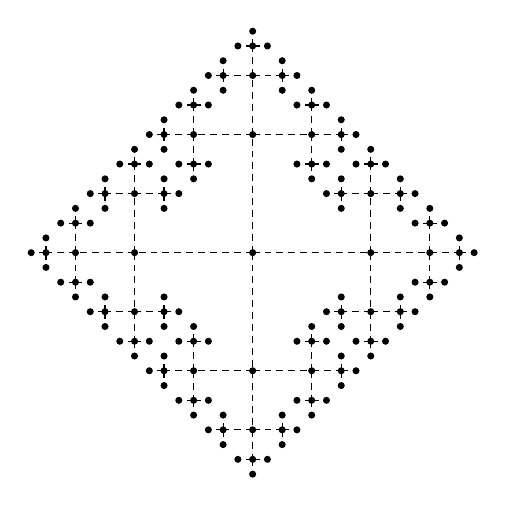
\begin{tikzpicture}[scale=1.5]
  \draw[dashed, dash pattern=on 2.5pt off 1.8pt, line width=0.45pt] (0.0000,0.0000) -- (1.0000,0.0000);
  \draw[dashed, dash pattern=on 2.5pt off 1.8pt, line width=0.45pt] (1.0000,0.0000) -- (1.5000,0.0000);
  \draw[dashed, dash pattern=on 2.5pt off 1.8pt, line width=0.45pt] (1.5000,0.0000) -- (1.7500,0.0000);
  \draw[dashed, dash pattern=on 2.5pt off 1.8pt, line width=0.45pt] (1.5000,0.0000) -- (1.5000,0.2500);
  \draw[dashed, dash pattern=on 2.5pt off 1.8pt, line width=0.45pt] (1.5000,0.0000) -- (1.5000,-0.2500);
  \draw[dashed, dash pattern=on 2.5pt off 1.8pt, line width=0.45pt] (1.0000,0.0000) -- (1.0000,0.5000);
  \draw[dashed, dash pattern=on 2.5pt off 1.8pt, line width=0.45pt] (1.0000,0.5000) -- (1.2500,0.5000);
  \draw[dashed, dash pattern=on 2.5pt off 1.8pt, line width=0.45pt] (1.0000,0.5000) -- (1.0000,0.7500);
  \draw[dashed, dash pattern=on 2.5pt off 1.8pt, line width=0.45pt] (1.0000,0.5000) -- (0.7500,0.5000);
  \draw[dashed, dash pattern=on 2.5pt off 1.8pt, line width=0.45pt] (1.0000,0.0000) -- (1.0000,-0.5000);
  \draw[dashed, dash pattern=on 2.5pt off 1.8pt, line width=0.45pt] (1.0000,-0.5000) -- (1.2500,-0.5000);
  \draw[dashed, dash pattern=on 2.5pt off 1.8pt, line width=0.45pt] (1.0000,-0.5000) -- (0.7500,-0.5000);
  \draw[dashed, dash pattern=on 2.5pt off 1.8pt, line width=0.45pt] (1.0000,-0.5000) -- (1.0000,-0.7500);
  \draw[dashed, dash pattern=on 2.5pt off 1.8pt, line width=0.45pt] (0.0000,0.0000) -- (0.0000,1.0000);
  \draw[dashed, dash pattern=on 2.5pt off 1.8pt, line width=0.45pt] (0.0000,1.0000) -- (0.5000,1.0000);
  \draw[dashed, dash pattern=on 2.5pt off 1.8pt, line width=0.45pt] (0.5000,1.0000) -- (0.7500,1.0000);
  \draw[dashed, dash pattern=on 2.5pt off 1.8pt, line width=0.45pt] (0.5000,1.0000) -- (0.5000,1.2500);
  \draw[dashed, dash pattern=on 2.5pt off 1.8pt, line width=0.45pt] (0.5000,1.0000) -- (0.5000,0.7500);
  \draw[dashed, dash pattern=on 2.5pt off 1.8pt, line width=0.45pt] (0.0000,1.0000) -- (0.0000,1.5000);
  \draw[dashed, dash pattern=on 2.5pt off 1.8pt, line width=0.45pt] (0.0000,1.5000) -- (0.2500,1.5000);
  \draw[dashed, dash pattern=on 2.5pt off 1.8pt, line width=0.45pt] (0.0000,1.5000) -- (0.0000,1.7500);
  \draw[dashed, dash pattern=on 2.5pt off 1.8pt, line width=0.45pt] (0.0000,1.5000) -- (-0.2500,1.5000);
  \draw[dashed, dash pattern=on 2.5pt off 1.8pt, line width=0.45pt] (0.0000,1.0000) -- (-0.5000,1.0000);
  \draw[dashed, dash pattern=on 2.5pt off 1.8pt, line width=0.45pt] (-0.5000,1.0000) -- (-0.5000,1.2500);
  \draw[dashed, dash pattern=on 2.5pt off 1.8pt, line width=0.45pt] (-0.5000,1.0000) -- (-0.7500,1.0000);
  \draw[dashed, dash pattern=on 2.5pt off 1.8pt, line width=0.45pt] (-0.5000,1.0000) -- (-0.5000,0.7500);
  \draw[dashed, dash pattern=on 2.5pt off 1.8pt, line width=0.45pt] (0.0000,0.0000) -- (-1.0000,0.0000);
  \draw[dashed, dash pattern=on 2.5pt off 1.8pt, line width=0.45pt] (-1.0000,0.0000) -- (-1.0000,0.5000);
  \draw[dashed, dash pattern=on 2.5pt off 1.8pt, line width=0.45pt] (-1.0000,0.5000) -- (-0.7500,0.5000);
  \draw[dashed, dash pattern=on 2.5pt off 1.8pt, line width=0.45pt] (-1.0000,0.5000) -- (-1.0000,0.7500);
  \draw[dashed, dash pattern=on 2.5pt off 1.8pt, line width=0.45pt] (-1.0000,0.5000) -- (-1.2500,0.5000);
  \draw[dashed, dash pattern=on 2.5pt off 1.8pt, line width=0.45pt] (-1.0000,0.0000) -- (-1.5000,0.0000);
  \draw[dashed, dash pattern=on 2.5pt off 1.8pt, line width=0.45pt] (-1.5000,0.0000) -- (-1.5000,0.2500);
  \draw[dashed, dash pattern=on 2.5pt off 1.8pt, line width=0.45pt] (-1.5000,0.0000) -- (-1.7500,0.0000);
  \draw[dashed, dash pattern=on 2.5pt off 1.8pt, line width=0.45pt] (-1.5000,0.0000) -- (-1.5000,-0.2500);
  \draw[dashed, dash pattern=on 2.5pt off 1.8pt, line width=0.45pt] (-1.0000,0.0000) -- (-1.0000,-0.5000);
  \draw[dashed, dash pattern=on 2.5pt off 1.8pt, line width=0.45pt] (-1.0000,-0.5000) -- (-0.7500,-0.5000);
  \draw[dashed, dash pattern=on 2.5pt off 1.8pt, line width=0.45pt] (-1.0000,-0.5000) -- (-1.2500,-0.5000);
  \draw[dashed, dash pattern=on 2.5pt off 1.8pt, line width=0.45pt] (-1.0000,-0.5000) -- (-1.0000,-0.7500);
  \draw[dashed, dash pattern=on 2.5pt off 1.8pt, line width=0.45pt] (0.0000,0.0000) -- (0.0000,-1.0000);
  \draw[dashed, dash pattern=on 2.5pt off 1.8pt, line width=0.45pt] (0.0000,-1.0000) -- (0.5000,-1.0000);
  \draw[dashed, dash pattern=on 2.5pt off 1.8pt, line width=0.45pt] (0.5000,-1.0000) -- (0.7500,-1.0000);
  \draw[dashed, dash pattern=on 2.5pt off 1.8pt, line width=0.45pt] (0.5000,-1.0000) -- (0.5000,-0.7500);
  \draw[dashed, dash pattern=on 2.5pt off 1.8pt, line width=0.45pt] (0.5000,-1.0000) -- (0.5000,-1.2500);
  \draw[dashed, dash pattern=on 2.5pt off 1.8pt, line width=0.45pt] (0.0000,-1.0000) -- (-0.5000,-1.0000);
  \draw[dashed, dash pattern=on 2.5pt off 1.8pt, line width=0.45pt] (-0.5000,-1.0000) -- (-0.5000,-0.7500);
  \draw[dashed, dash pattern=on 2.5pt off 1.8pt, line width=0.45pt] (-0.5000,-1.0000) -- (-0.7500,-1.0000);
  \draw[dashed, dash pattern=on 2.5pt off 1.8pt, line width=0.45pt] (-0.5000,-1.0000) -- (-0.5000,-1.2500);
  \draw[dashed, dash pattern=on 2.5pt off 1.8pt, line width=0.45pt] (0.0000,-1.0000) -- (0.0000,-1.5000);
  \draw[dashed, dash pattern=on 2.5pt off 1.8pt, line width=0.45pt] (0.0000,-1.5000) -- (0.2500,-1.5000);
  \draw[dashed, dash pattern=on 2.5pt off 1.8pt, line width=0.45pt] (0.0000,-1.5000) -- (-0.2500,-1.5000);
  \draw[dashed, dash pattern=on 2.5pt off 1.8pt, line width=0.45pt] (0.0000,-1.5000) -- (0.0000,-1.7500);
  \fill (0.0000,0.0000) circle (.85pt);
  \fill (1.0000,0.0000) circle (.85pt);
  \fill (1.5000,0.0000) circle (.85pt);
  \fill (1.7500,0.0000) circle (.85pt);
  \fill (1.5000,0.2500) circle (.85pt);
  \fill (1.5000,-0.2500) circle (.85pt);
  \fill (1.0000,0.5000) circle (.85pt);
  \fill (1.2500,0.5000) circle (.85pt);
  \fill (1.0000,0.7500) circle (.85pt);
  \fill (0.7500,0.5000) circle (.85pt);
  \fill (1.0000,-0.5000) circle (.85pt);
  \fill (1.2500,-0.5000) circle (.85pt);
  \fill (0.7500,-0.5000) circle (.85pt);
  \fill (1.0000,-0.7500) circle (.85pt);
  \fill (0.0000,1.0000) circle (.85pt);
  \fill (0.5000,1.0000) circle (.85pt);
  \fill (0.7500,1.0000) circle (.85pt);
  \fill (0.5000,1.2500) circle (.85pt);
  \fill (0.5000,0.7500) circle (.85pt);
  \fill (0.0000,1.5000) circle (.85pt);
  \fill (0.2500,1.5000) circle (.85pt);
  \fill (0.0000,1.7500) circle (.85pt);
  \fill (-0.2500,1.5000) circle (.85pt);
  \fill (-0.5000,1.0000) circle (.85pt);
  \fill (-0.5000,1.2500) circle (.85pt);
  \fill (-0.7500,1.0000) circle (.85pt);
  \fill (-0.5000,0.7500) circle (.85pt);
  \fill (-1.0000,0.0000) circle (.85pt);
  \fill (-1.0000,0.5000) circle (.85pt);
  \fill (-0.7500,0.5000) circle (.85pt);
  \fill (-1.0000,0.7500) circle (.85pt);
  \fill (-1.2500,0.5000) circle (.85pt);
  \fill (-1.5000,0.0000) circle (.85pt);
  \fill (-1.5000,0.2500) circle (.85pt);
  \fill (-1.7500,0.0000) circle (.85pt);
  \fill (-1.5000,-0.2500) circle (.85pt);
  \fill (-1.0000,-0.5000) circle (.85pt);
  \fill (-0.7500,-0.5000) circle (.85pt);
  \fill (-1.2500,-0.5000) circle (.85pt);
  \fill (-1.0000,-0.7500) circle (.85pt);
  \fill (0.0000,-1.0000) circle (.85pt);
  \fill (0.5000,-1.0000) circle (.85pt);
  \fill (0.7500,-1.0000) circle (.85pt);
  \fill (0.5000,-0.7500) circle (.85pt);
  \fill (0.5000,-1.2500) circle (.85pt);
  \fill (-0.5000,-1.0000) circle (.85pt);
  \fill (-0.5000,-0.7500) circle (.85pt);
  \fill (-0.7500,-1.0000) circle (.85pt);
  \fill (-0.5000,-1.2500) circle (.85pt);
  \fill (0.0000,-1.5000) circle (.85pt);
  \fill (0.2500,-1.5000) circle (.85pt);
  \fill (-0.2500,-1.5000) circle (.85pt);
  \fill (0.0000,-1.7500) circle (.85pt);
  \draw[dashed, dash pattern=on 2.5pt off 1.8pt, line width=0.45pt] (1.7500,0.0000) -- (1.8750,0.0000);
  \fill (1.8750,0.0000) circle (.85pt);
  \draw[dashed, dash pattern=on 2.5pt off 1.8pt, line width=0.45pt] (1.7500,0.0000) -- (1.7500,0.1250);
  \fill (1.7500,0.1250) circle (.85pt);
  \draw[dashed, dash pattern=on 2.5pt off 1.8pt, line width=0.45pt] (1.7500,0.0000) -- (1.7500,-0.1250);
  \fill (1.7500,-0.1250) circle (.85pt);
  \draw[dashed, dash pattern=on 2.5pt off 1.8pt, line width=0.45pt] (1.5000,0.2500) -- (1.6250,0.2500);
  \fill (1.6250,0.2500) circle (.85pt);
  \draw[dashed, dash pattern=on 2.5pt off 1.8pt, line width=0.45pt] (1.5000,0.2500) -- (1.3750,0.2500);
  \fill (1.3750,0.2500) circle (.85pt);
  \draw[dashed, dash pattern=on 2.5pt off 1.8pt, line width=0.45pt] (1.5000,0.2500) -- (1.5000,0.3750);
  \fill (1.5000,0.3750) circle (.85pt);
  \draw[dashed, dash pattern=on 2.5pt off 1.8pt, line width=0.45pt] (1.5000,-0.2500) -- (1.6250,-0.2500);
  \fill (1.6250,-0.2500) circle (.85pt);
  \draw[dashed, dash pattern=on 2.5pt off 1.8pt, line width=0.45pt] (1.5000,-0.2500) -- (1.3750,-0.2500);
  \fill (1.3750,-0.2500) circle (.85pt);
  \draw[dashed, dash pattern=on 2.5pt off 1.8pt, line width=0.45pt] (1.5000,-0.2500) -- (1.5000,-0.3750);
  \fill (1.5000,-0.3750) circle (.85pt);
  \draw[dashed, dash pattern=on 2.5pt off 1.8pt, line width=0.45pt] (1.2500,0.5000) -- (1.3750,0.5000);
  \fill (1.3750,0.5000) circle (.85pt);
  \draw[dashed, dash pattern=on 2.5pt off 1.8pt, line width=0.45pt] (1.2500,0.5000) -- (1.2500,0.6250);
  \fill (1.2500,0.6250) circle (.85pt);
  \draw[dashed, dash pattern=on 2.5pt off 1.8pt, line width=0.45pt] (1.2500,0.5000) -- (1.2500,0.3750);
  \fill (1.2500,0.3750) circle (.85pt);
  \draw[dashed, dash pattern=on 2.5pt off 1.8pt, line width=0.45pt] (1.0000,0.7500) -- (1.1250,0.7500);
  \fill (1.1250,0.7500) circle (.85pt);
  \draw[dashed, dash pattern=on 2.5pt off 1.8pt, line width=0.45pt] (1.0000,0.7500) -- (0.8750,0.7500);
  \fill (0.8750,0.7500) circle (.85pt);
  \draw[dashed, dash pattern=on 2.5pt off 1.8pt, line width=0.45pt] (1.0000,0.7500) -- (1.0000,0.8750);
  \fill (1.0000,0.8750) circle (.85pt);
  \draw[dashed, dash pattern=on 2.5pt off 1.8pt, line width=0.45pt] (0.7500,0.5000) -- (0.6250,0.5000);
  \fill (0.6250,0.5000) circle (.85pt);
  \draw[dashed, dash pattern=on 2.5pt off 1.8pt, line width=0.45pt] (0.7500,0.5000) -- (0.7500,0.6250);
  \fill (0.7500,0.6250) circle (.85pt);
  \draw[dashed, dash pattern=on 2.5pt off 1.8pt, line width=0.45pt] (0.7500,0.5000) -- (0.7500,0.3750);
  \fill (0.7500,0.3750) circle (.85pt);
  \draw[dashed, dash pattern=on 2.5pt off 1.8pt, line width=0.45pt] (1.2500,-0.5000) -- (1.3750,-0.5000);
  \fill (1.3750,-0.5000) circle (.85pt);
  \draw[dashed, dash pattern=on 2.5pt off 1.8pt, line width=0.45pt] (1.2500,-0.5000) -- (1.2500,-0.3750);
  \fill (1.2500,-0.3750) circle (.85pt);
  \draw[dashed, dash pattern=on 2.5pt off 1.8pt, line width=0.45pt] (1.2500,-0.5000) -- (1.2500,-0.6250);
  \fill (1.2500,-0.6250) circle (.85pt);
  \draw[dashed, dash pattern=on 2.5pt off 1.8pt, line width=0.45pt] (0.7500,-0.5000) -- (0.6250,-0.5000);
  \fill (0.6250,-0.5000) circle (.85pt);
  \draw[dashed, dash pattern=on 2.5pt off 1.8pt, line width=0.45pt] (0.7500,-0.5000) -- (0.7500,-0.3750);
  \fill (0.7500,-0.3750) circle (.85pt);
  \draw[dashed, dash pattern=on 2.5pt off 1.8pt, line width=0.45pt] (0.7500,-0.5000) -- (0.7500,-0.6250);
  \fill (0.7500,-0.6250) circle (.85pt);
  \draw[dashed, dash pattern=on 2.5pt off 1.8pt, line width=0.45pt] (1.0000,-0.7500) -- (1.1250,-0.7500);
  \fill (1.1250,-0.7500) circle (.85pt);
  \draw[dashed, dash pattern=on 2.5pt off 1.8pt, line width=0.45pt] (1.0000,-0.7500) -- (0.8750,-0.7500);
  \fill (0.8750,-0.7500) circle (.85pt);
  \draw[dashed, dash pattern=on 2.5pt off 1.8pt, line width=0.45pt] (1.0000,-0.7500) -- (1.0000,-0.8750);
  \fill (1.0000,-0.8750) circle (.85pt);
  \draw[dashed, dash pattern=on 2.5pt off 1.8pt, line width=0.45pt] (0.7500,1.0000) -- (0.8750,1.0000);
  \fill (0.8750,1.0000) circle (.85pt);
  \draw[dashed, dash pattern=on 2.5pt off 1.8pt, line width=0.45pt] (0.7500,1.0000) -- (0.7500,1.1250);
  \fill (0.7500,1.1250) circle (.85pt);
  \draw[dashed, dash pattern=on 2.5pt off 1.8pt, line width=0.45pt] (0.7500,1.0000) -- (0.7500,0.8750);
  \fill (0.7500,0.8750) circle (.85pt);
  \draw[dashed, dash pattern=on 2.5pt off 1.8pt, line width=0.45pt] (0.5000,1.2500) -- (0.6250,1.2500);
  \fill (0.6250,1.2500) circle (.85pt);
  \draw[dashed, dash pattern=on 2.5pt off 1.8pt, line width=0.45pt] (0.5000,1.2500) -- (0.3750,1.2500);
  \fill (0.3750,1.2500) circle (.85pt);
  \draw[dashed, dash pattern=on 2.5pt off 1.8pt, line width=0.45pt] (0.5000,1.2500) -- (0.5000,1.3750);
  \fill (0.5000,1.3750) circle (.85pt);
  \draw[dashed, dash pattern=on 2.5pt off 1.8pt, line width=0.45pt] (0.5000,0.7500) -- (0.6250,0.7500);
  \fill (0.6250,0.7500) circle (.85pt);
  \draw[dashed, dash pattern=on 2.5pt off 1.8pt, line width=0.45pt] (0.5000,0.7500) -- (0.3750,0.7500);
  \fill (0.3750,0.7500) circle (.85pt);
  \draw[dashed, dash pattern=on 2.5pt off 1.8pt, line width=0.45pt] (0.5000,0.7500) -- (0.5000,0.6250);
  \fill (0.5000,0.6250) circle (.85pt);
  \draw[dashed, dash pattern=on 2.5pt off 1.8pt, line width=0.45pt] (0.2500,1.5000) -- (0.3750,1.5000);
  \fill (0.3750,1.5000) circle (.85pt);
  \draw[dashed, dash pattern=on 2.5pt off 1.8pt, line width=0.45pt] (0.2500,1.5000) -- (0.2500,1.6250);
  \fill (0.2500,1.6250) circle (.85pt);
  \draw[dashed, dash pattern=on 2.5pt off 1.8pt, line width=0.45pt] (0.2500,1.5000) -- (0.2500,1.3750);
  \fill (0.2500,1.3750) circle (.85pt);
  \draw[dashed, dash pattern=on 2.5pt off 1.8pt, line width=0.45pt] (0.0000,1.7500) -- (0.1250,1.7500);
  \fill (0.1250,1.7500) circle (.85pt);
  \draw[dashed, dash pattern=on 2.5pt off 1.8pt, line width=0.45pt] (0.0000,1.7500) -- (-0.1250,1.7500);
  \fill (-0.1250,1.7500) circle (.85pt);
  \draw[dashed, dash pattern=on 2.5pt off 1.8pt, line width=0.45pt] (0.0000,1.7500) -- (0.0000,1.8750);
  \fill (0.0000,1.8750) circle (.85pt);
  \draw[dashed, dash pattern=on 2.5pt off 1.8pt, line width=0.45pt] (-0.2500,1.5000) -- (-0.3750,1.5000);
  \fill (-0.3750,1.5000) circle (.85pt);
  \draw[dashed, dash pattern=on 2.5pt off 1.8pt, line width=0.45pt] (-0.2500,1.5000) -- (-0.2500,1.6250);
  \fill (-0.2500,1.6250) circle (.85pt);
  \draw[dashed, dash pattern=on 2.5pt off 1.8pt, line width=0.45pt] (-0.2500,1.5000) -- (-0.2500,1.3750);
  \fill (-0.2500,1.3750) circle (.85pt);
  \draw[dashed, dash pattern=on 2.5pt off 1.8pt, line width=0.45pt] (-0.5000,1.2500) -- (-0.3750,1.2500);
  \fill (-0.3750,1.2500) circle (.85pt);
  \draw[dashed, dash pattern=on 2.5pt off 1.8pt, line width=0.45pt] (-0.5000,1.2500) -- (-0.6250,1.2500);
  \fill (-0.6250,1.2500) circle (.85pt);
  \draw[dashed, dash pattern=on 2.5pt off 1.8pt, line width=0.45pt] (-0.5000,1.2500) -- (-0.5000,1.3750);
  \fill (-0.5000,1.3750) circle (.85pt);
  \draw[dashed, dash pattern=on 2.5pt off 1.8pt, line width=0.45pt] (-0.7500,1.0000) -- (-0.8750,1.0000);
  \fill (-0.8750,1.0000) circle (.85pt);
  \draw[dashed, dash pattern=on 2.5pt off 1.8pt, line width=0.45pt] (-0.7500,1.0000) -- (-0.7500,1.1250);
  \fill (-0.7500,1.1250) circle (.85pt);
  \draw[dashed, dash pattern=on 2.5pt off 1.8pt, line width=0.45pt] (-0.7500,1.0000) -- (-0.7500,0.8750);
  \fill (-0.7500,0.8750) circle (.85pt);
  \draw[dashed, dash pattern=on 2.5pt off 1.8pt, line width=0.45pt] (-0.5000,0.7500) -- (-0.3750,0.7500);
  \fill (-0.3750,0.7500) circle (.85pt);
  \draw[dashed, dash pattern=on 2.5pt off 1.8pt, line width=0.45pt] (-0.5000,0.7500) -- (-0.6250,0.7500);
  \fill (-0.6250,0.7500) circle (.85pt);
  \draw[dashed, dash pattern=on 2.5pt off 1.8pt, line width=0.45pt] (-0.5000,0.7500) -- (-0.5000,0.6250);
  \fill (-0.5000,0.6250) circle (.85pt);
  \draw[dashed, dash pattern=on 2.5pt off 1.8pt, line width=0.45pt] (-0.7500,0.5000) -- (-0.6250,0.5000);
  \fill (-0.6250,0.5000) circle (.85pt);
  \draw[dashed, dash pattern=on 2.5pt off 1.8pt, line width=0.45pt] (-0.7500,0.5000) -- (-0.7500,0.6250);
  \fill (-0.7500,0.6250) circle (.85pt);
  \draw[dashed, dash pattern=on 2.5pt off 1.8pt, line width=0.45pt] (-0.7500,0.5000) -- (-0.7500,0.3750);
  \fill (-0.7500,0.3750) circle (.85pt);
  \draw[dashed, dash pattern=on 2.5pt off 1.8pt, line width=0.45pt] (-1.0000,0.7500) -- (-0.8750,0.7500);
  \fill (-0.8750,0.7500) circle (.85pt);
  \draw[dashed, dash pattern=on 2.5pt off 1.8pt, line width=0.45pt] (-1.0000,0.7500) -- (-1.1250,0.7500);
  \fill (-1.1250,0.7500) circle (.85pt);
  \draw[dashed, dash pattern=on 2.5pt off 1.8pt, line width=0.45pt] (-1.0000,0.7500) -- (-1.0000,0.8750);
  \fill (-1.0000,0.8750) circle (.85pt);
  \draw[dashed, dash pattern=on 2.5pt off 1.8pt, line width=0.45pt] (-1.2500,0.5000) -- (-1.3750,0.5000);
  \fill (-1.3750,0.5000) circle (.85pt);
  \draw[dashed, dash pattern=on 2.5pt off 1.8pt, line width=0.45pt] (-1.2500,0.5000) -- (-1.2500,0.6250);
  \fill (-1.2500,0.6250) circle (.85pt);
  \draw[dashed, dash pattern=on 2.5pt off 1.8pt, line width=0.45pt] (-1.2500,0.5000) -- (-1.2500,0.3750);
  \fill (-1.2500,0.3750) circle (.85pt);
  \draw[dashed, dash pattern=on 2.5pt off 1.8pt, line width=0.45pt] (-1.5000,0.2500) -- (-1.3750,0.2500);
  \fill (-1.3750,0.2500) circle (.85pt);
  \draw[dashed, dash pattern=on 2.5pt off 1.8pt, line width=0.45pt] (-1.5000,0.2500) -- (-1.6250,0.2500);
  \fill (-1.6250,0.2500) circle (.85pt);
  \draw[dashed, dash pattern=on 2.5pt off 1.8pt, line width=0.45pt] (-1.5000,0.2500) -- (-1.5000,0.3750);
  \fill (-1.5000,0.3750) circle (.85pt);
  \draw[dashed, dash pattern=on 2.5pt off 1.8pt, line width=0.45pt] (-1.7500,0.0000) -- (-1.8750,0.0000);
  \fill (-1.8750,0.0000) circle (.85pt);
  \draw[dashed, dash pattern=on 2.5pt off 1.8pt, line width=0.45pt] (-1.7500,0.0000) -- (-1.7500,0.1250);
  \fill (-1.7500,0.1250) circle (.85pt);
  \draw[dashed, dash pattern=on 2.5pt off 1.8pt, line width=0.45pt] (-1.7500,0.0000) -- (-1.7500,-0.1250);
  \fill (-1.7500,-0.1250) circle (.85pt);
  \draw[dashed, dash pattern=on 2.5pt off 1.8pt, line width=0.45pt] (-1.5000,-0.2500) -- (-1.3750,-0.2500);
  \fill (-1.3750,-0.2500) circle (.85pt);
  \draw[dashed, dash pattern=on 2.5pt off 1.8pt, line width=0.45pt] (-1.5000,-0.2500) -- (-1.6250,-0.2500);
  \fill (-1.6250,-0.2500) circle (.85pt);
  \draw[dashed, dash pattern=on 2.5pt off 1.8pt, line width=0.45pt] (-1.5000,-0.2500) -- (-1.5000,-0.3750);
  \fill (-1.5000,-0.3750) circle (.85pt);
  \draw[dashed, dash pattern=on 2.5pt off 1.8pt, line width=0.45pt] (-0.7500,-0.5000) -- (-0.6250,-0.5000);
  \fill (-0.6250,-0.5000) circle (.85pt);
  \draw[dashed, dash pattern=on 2.5pt off 1.8pt, line width=0.45pt] (-0.7500,-0.5000) -- (-0.7500,-0.3750);
  \fill (-0.7500,-0.3750) circle (.85pt);
  \draw[dashed, dash pattern=on 2.5pt off 1.8pt, line width=0.45pt] (-0.7500,-0.5000) -- (-0.7500,-0.6250);
  \fill (-0.7500,-0.6250) circle (.85pt);
  \draw[dashed, dash pattern=on 2.5pt off 1.8pt, line width=0.45pt] (-1.2500,-0.5000) -- (-1.3750,-0.5000);
  \fill (-1.3750,-0.5000) circle (.85pt);
  \draw[dashed, dash pattern=on 2.5pt off 1.8pt, line width=0.45pt] (-1.2500,-0.5000) -- (-1.2500,-0.3750);
  \fill (-1.2500,-0.3750) circle (.85pt);
  \draw[dashed, dash pattern=on 2.5pt off 1.8pt, line width=0.45pt] (-1.2500,-0.5000) -- (-1.2500,-0.6250);
  \fill (-1.2500,-0.6250) circle (.85pt);
  \draw[dashed, dash pattern=on 2.5pt off 1.8pt, line width=0.45pt] (-1.0000,-0.7500) -- (-0.8750,-0.7500);
  \fill (-0.8750,-0.7500) circle (.85pt);
  \draw[dashed, dash pattern=on 2.5pt off 1.8pt, line width=0.45pt] (-1.0000,-0.7500) -- (-1.1250,-0.7500);
  \fill (-1.1250,-0.7500) circle (.85pt);
  \draw[dashed, dash pattern=on 2.5pt off 1.8pt, line width=0.45pt] (-1.0000,-0.7500) -- (-1.0000,-0.8750);
  \fill (-1.0000,-0.8750) circle (.85pt);
  \draw[dashed, dash pattern=on 2.5pt off 1.8pt, line width=0.45pt] (0.7500,-1.0000) -- (0.8750,-1.0000);
  \fill (0.8750,-1.0000) circle (.85pt);
  \draw[dashed, dash pattern=on 2.5pt off 1.8pt, line width=0.45pt] (0.7500,-1.0000) -- (0.7500,-0.8750);
  \fill (0.7500,-0.8750) circle (.85pt);
  \draw[dashed, dash pattern=on 2.5pt off 1.8pt, line width=0.45pt] (0.7500,-1.0000) -- (0.7500,-1.1250);
  \fill (0.7500,-1.1250) circle (.85pt);
  \draw[dashed, dash pattern=on 2.5pt off 1.8pt, line width=0.45pt] (0.5000,-0.7500) -- (0.6250,-0.7500);
  \fill (0.6250,-0.7500) circle (.85pt);
  \draw[dashed, dash pattern=on 2.5pt off 1.8pt, line width=0.45pt] (0.5000,-0.7500) -- (0.3750,-0.7500);
  \fill (0.3750,-0.7500) circle (.85pt);
  \draw[dashed, dash pattern=on 2.5pt off 1.8pt, line width=0.45pt] (0.5000,-0.7500) -- (0.5000,-0.6250);
  \fill (0.5000,-0.6250) circle (.85pt);
  \draw[dashed, dash pattern=on 2.5pt off 1.8pt, line width=0.45pt] (0.5000,-1.2500) -- (0.6250,-1.2500);
  \fill (0.6250,-1.2500) circle (.85pt);
  \draw[dashed, dash pattern=on 2.5pt off 1.8pt, line width=0.45pt] (0.5000,-1.2500) -- (0.3750,-1.2500);
  \fill (0.3750,-1.2500) circle (.85pt);
  \draw[dashed, dash pattern=on 2.5pt off 1.8pt, line width=0.45pt] (0.5000,-1.2500) -- (0.5000,-1.3750);
  \fill (0.5000,-1.3750) circle (.85pt);
  \draw[dashed, dash pattern=on 2.5pt off 1.8pt, line width=0.45pt] (-0.5000,-0.7500) -- (-0.3750,-0.7500);
  \fill (-0.3750,-0.7500) circle (.85pt);
  \draw[dashed, dash pattern=on 2.5pt off 1.8pt, line width=0.45pt] (-0.5000,-0.7500) -- (-0.6250,-0.7500);
  \fill (-0.6250,-0.7500) circle (.85pt);
  \draw[dashed, dash pattern=on 2.5pt off 1.8pt, line width=0.45pt] (-0.5000,-0.7500) -- (-0.5000,-0.6250);
  \fill (-0.5000,-0.6250) circle (.85pt);
  \draw[dashed, dash pattern=on 2.5pt off 1.8pt, line width=0.45pt] (-0.7500,-1.0000) -- (-0.8750,-1.0000);
  \fill (-0.8750,-1.0000) circle (.85pt);
  \draw[dashed, dash pattern=on 2.5pt off 1.8pt, line width=0.45pt] (-0.7500,-1.0000) -- (-0.7500,-0.8750);
  \fill (-0.7500,-0.8750) circle (.85pt);
  \draw[dashed, dash pattern=on 2.5pt off 1.8pt, line width=0.45pt] (-0.7500,-1.0000) -- (-0.7500,-1.1250);
  \fill (-0.7500,-1.1250) circle (.85pt);
  \draw[dashed, dash pattern=on 2.5pt off 1.8pt, line width=0.45pt] (-0.5000,-1.2500) -- (-0.3750,-1.2500);
  \fill (-0.3750,-1.2500) circle (.85pt);
  \draw[dashed, dash pattern=on 2.5pt off 1.8pt, line width=0.45pt] (-0.5000,-1.2500) -- (-0.6250,-1.2500);
  \fill (-0.6250,-1.2500) circle (.85pt);
  \draw[dashed, dash pattern=on 2.5pt off 1.8pt, line width=0.45pt] (-0.5000,-1.2500) -- (-0.5000,-1.3750);
  \fill (-0.5000,-1.3750) circle (.85pt);
  \draw[dashed, dash pattern=on 2.5pt off 1.8pt, line width=0.45pt] (0.2500,-1.5000) -- (0.3750,-1.5000);
  \fill (0.3750,-1.5000) circle (.85pt);
  \draw[dashed, dash pattern=on 2.5pt off 1.8pt, line width=0.45pt] (0.2500,-1.5000) -- (0.2500,-1.3750);
  \fill (0.2500,-1.3750) circle (.85pt);
  \draw[dashed, dash pattern=on 2.5pt off 1.8pt, line width=0.45pt] (0.2500,-1.5000) -- (0.2500,-1.6250);
  \fill (0.2500,-1.6250) circle (.85pt);
  \draw[dashed, dash pattern=on 2.5pt off 1.8pt, line width=0.45pt] (-0.2500,-1.5000) -- (-0.3750,-1.5000);
  \fill (-0.3750,-1.5000) circle (.85pt);
  \draw[dashed, dash pattern=on 2.5pt off 1.8pt, line width=0.45pt] (-0.2500,-1.5000) -- (-0.2500,-1.3750);
  \fill (-0.2500,-1.3750) circle (.85pt);
  \draw[dashed, dash pattern=on 2.5pt off 1.8pt, line width=0.45pt] (-0.2500,-1.5000) -- (-0.2500,-1.6250);
  \fill (-0.2500,-1.6250) circle (.85pt);
  \draw[dashed, dash pattern=on 2.5pt off 1.8pt, line width=0.45pt] (0.0000,-1.7500) -- (0.1250,-1.7500);
  \fill (0.1250,-1.7500) circle (.85pt);
  \draw[dashed, dash pattern=on 2.5pt off 1.8pt, line width=0.45pt] (0.0000,-1.7500) -- (-0.1250,-1.7500);
  \fill (-0.1250,-1.7500) circle (.85pt);
  \draw[dashed, dash pattern=on 2.5pt off 1.8pt, line width=0.45pt] (0.0000,-1.7500) -- (0.0000,-1.8750);
  \fill (0.0000,-1.8750) circle (.85pt);
\end{tikzpicture}
\]

它从一点 (图的中心) 出发, 向四个方向各伸出长度 $1$ 的分支, 然后类似地伸出长度 $1/2$ 的分支, 再 $1/4$, 再 $1/8$, 再\ldots (我们到此为止, 以免把图弄得过于杂乱). 于是, $F(\{x, y\})$ 的每个元素都以相当自然的方式对应于这张图中恰好一个点. 的确, 我们可以把空词放在中心; 并约定: 词中每个 $x$ 使我们向右走一步, 每个 $x^{-1}$ 向左, 每个 $y$ 向上, 每个 $y^{-1}$ 向下. 比如, 词 $yx^{-1}yx$ 把我们带到这里:
\[
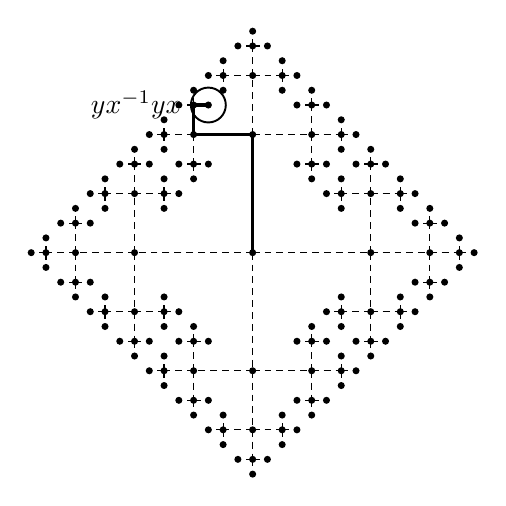
\begin{tikzpicture}[scale=1.5]
  \draw[dashed, dash pattern=on 2.5pt off 1.8pt, line width=0.45pt] (0.0000,0.0000) -- (1.0000,0.0000);
  \draw[dashed, dash pattern=on 2.5pt off 1.8pt, line width=0.45pt] (1.0000,0.0000) -- (1.5000,0.0000);
  \draw[dashed, dash pattern=on 2.5pt off 1.8pt, line width=0.45pt] (1.5000,0.0000) -- (1.7500,0.0000);
  \draw[dashed, dash pattern=on 2.5pt off 1.8pt, line width=0.45pt] (1.5000,0.0000) -- (1.5000,0.2500);
  \draw[dashed, dash pattern=on 2.5pt off 1.8pt, line width=0.45pt] (1.5000,0.0000) -- (1.5000,-0.2500);
  \draw[dashed, dash pattern=on 2.5pt off 1.8pt, line width=0.45pt] (1.0000,0.0000) -- (1.0000,0.5000);
  \draw[dashed, dash pattern=on 2.5pt off 1.8pt, line width=0.45pt] (1.0000,0.5000) -- (1.2500,0.5000);
  \draw[dashed, dash pattern=on 2.5pt off 1.8pt, line width=0.45pt] (1.0000,0.5000) -- (1.0000,0.7500);
  \draw[dashed, dash pattern=on 2.5pt off 1.8pt, line width=0.45pt] (1.0000,0.5000) -- (0.7500,0.5000);
  \draw[dashed, dash pattern=on 2.5pt off 1.8pt, line width=0.45pt] (1.0000,0.0000) -- (1.0000,-0.5000);
  \draw[dashed, dash pattern=on 2.5pt off 1.8pt, line width=0.45pt] (1.0000,-0.5000) -- (1.2500,-0.5000);
  \draw[dashed, dash pattern=on 2.5pt off 1.8pt, line width=0.45pt] (1.0000,-0.5000) -- (0.7500,-0.5000);
  \draw[dashed, dash pattern=on 2.5pt off 1.8pt, line width=0.45pt] (1.0000,-0.5000) -- (1.0000,-0.7500);
  \draw[dashed, dash pattern=on 2.5pt off 1.8pt, line width=0.45pt] (0.0000,0.0000) -- (0.0000,1.0000);
  \draw[dashed, dash pattern=on 2.5pt off 1.8pt, line width=0.45pt] (0.0000,1.0000) -- (0.5000,1.0000);
  \draw[dashed, dash pattern=on 2.5pt off 1.8pt, line width=0.45pt] (0.5000,1.0000) -- (0.7500,1.0000);
  \draw[dashed, dash pattern=on 2.5pt off 1.8pt, line width=0.45pt] (0.5000,1.0000) -- (0.5000,1.2500);
  \draw[dashed, dash pattern=on 2.5pt off 1.8pt, line width=0.45pt] (0.5000,1.0000) -- (0.5000,0.7500);
  \draw[dashed, dash pattern=on 2.5pt off 1.8pt, line width=0.45pt] (0.0000,1.0000) -- (0.0000,1.5000);
  \draw[dashed, dash pattern=on 2.5pt off 1.8pt, line width=0.45pt] (0.0000,1.5000) -- (0.2500,1.5000);
  \draw[dashed, dash pattern=on 2.5pt off 1.8pt, line width=0.45pt] (0.0000,1.5000) -- (0.0000,1.7500);
  \draw[dashed, dash pattern=on 2.5pt off 1.8pt, line width=0.45pt] (0.0000,1.5000) -- (-0.2500,1.5000);
  \draw[dashed, dash pattern=on 2.5pt off 1.8pt, line width=0.45pt] (0.0000,1.0000) -- (-0.5000,1.0000);
  \draw[dashed, dash pattern=on 2.5pt off 1.8pt, line width=0.45pt] (-0.5000,1.0000) -- (-0.5000,1.2500);
  \draw[dashed, dash pattern=on 2.5pt off 1.8pt, line width=0.45pt] (-0.5000,1.0000) -- (-0.7500,1.0000);
  \draw[dashed, dash pattern=on 2.5pt off 1.8pt, line width=0.45pt] (-0.5000,1.0000) -- (-0.5000,0.7500);
  \draw[dashed, dash pattern=on 2.5pt off 1.8pt, line width=0.45pt] (0.0000,0.0000) -- (-1.0000,0.0000);
  \draw[dashed, dash pattern=on 2.5pt off 1.8pt, line width=0.45pt] (-1.0000,0.0000) -- (-1.0000,0.5000);
  \draw[dashed, dash pattern=on 2.5pt off 1.8pt, line width=0.45pt] (-1.0000,0.5000) -- (-0.7500,0.5000);
  \draw[dashed, dash pattern=on 2.5pt off 1.8pt, line width=0.45pt] (-1.0000,0.5000) -- (-1.0000,0.7500);
  \draw[dashed, dash pattern=on 2.5pt off 1.8pt, line width=0.45pt] (-1.0000,0.5000) -- (-1.2500,0.5000);
  \draw[dashed, dash pattern=on 2.5pt off 1.8pt, line width=0.45pt] (-1.0000,0.0000) -- (-1.5000,0.0000);
  \draw[dashed, dash pattern=on 2.5pt off 1.8pt, line width=0.45pt] (-1.5000,0.0000) -- (-1.5000,0.2500);
  \draw[dashed, dash pattern=on 2.5pt off 1.8pt, line width=0.45pt] (-1.5000,0.0000) -- (-1.7500,0.0000);
  \draw[dashed, dash pattern=on 2.5pt off 1.8pt, line width=0.45pt] (-1.5000,0.0000) -- (-1.5000,-0.2500);
  \draw[dashed, dash pattern=on 2.5pt off 1.8pt, line width=0.45pt] (-1.0000,0.0000) -- (-1.0000,-0.5000);
  \draw[dashed, dash pattern=on 2.5pt off 1.8pt, line width=0.45pt] (-1.0000,-0.5000) -- (-0.7500,-0.5000);
  \draw[dashed, dash pattern=on 2.5pt off 1.8pt, line width=0.45pt] (-1.0000,-0.5000) -- (-1.2500,-0.5000);
  \draw[dashed, dash pattern=on 2.5pt off 1.8pt, line width=0.45pt] (-1.0000,-0.5000) -- (-1.0000,-0.7500);
  \draw[dashed, dash pattern=on 2.5pt off 1.8pt, line width=0.45pt] (0.0000,0.0000) -- (0.0000,-1.0000);
  \draw[dashed, dash pattern=on 2.5pt off 1.8pt, line width=0.45pt] (0.0000,-1.0000) -- (0.5000,-1.0000);
  \draw[dashed, dash pattern=on 2.5pt off 1.8pt, line width=0.45pt] (0.5000,-1.0000) -- (0.7500,-1.0000);
  \draw[dashed, dash pattern=on 2.5pt off 1.8pt, line width=0.45pt] (0.5000,-1.0000) -- (0.5000,-0.7500);
  \draw[dashed, dash pattern=on 2.5pt off 1.8pt, line width=0.45pt] (0.5000,-1.0000) -- (0.5000,-1.2500);
  \draw[dashed, dash pattern=on 2.5pt off 1.8pt, line width=0.45pt] (0.0000,-1.0000) -- (-0.5000,-1.0000);
  \draw[dashed, dash pattern=on 2.5pt off 1.8pt, line width=0.45pt] (-0.5000,-1.0000) -- (-0.5000,-0.7500);
  \draw[dashed, dash pattern=on 2.5pt off 1.8pt, line width=0.45pt] (-0.5000,-1.0000) -- (-0.7500,-1.0000);
  \draw[dashed, dash pattern=on 2.5pt off 1.8pt, line width=0.45pt] (-0.5000,-1.0000) -- (-0.5000,-1.2500);
  \draw[dashed, dash pattern=on 2.5pt off 1.8pt, line width=0.45pt] (0.0000,-1.0000) -- (0.0000,-1.5000);
  \draw[dashed, dash pattern=on 2.5pt off 1.8pt, line width=0.45pt] (0.0000,-1.5000) -- (0.2500,-1.5000);
  \draw[dashed, dash pattern=on 2.5pt off 1.8pt, line width=0.45pt] (0.0000,-1.5000) -- (-0.2500,-1.5000);
  \draw[dashed, dash pattern=on 2.5pt off 1.8pt, line width=0.45pt] (0.0000,-1.5000) -- (0.0000,-1.7500);
  \fill (0.0000,0.0000) circle (.85pt);
  \fill (1.0000,0.0000) circle (.85pt);
  \fill (1.5000,0.0000) circle (.85pt);
  \fill (1.7500,0.0000) circle (.85pt);
  \fill (1.5000,0.2500) circle (.85pt);
  \fill (1.5000,-0.2500) circle (.85pt);
  \fill (1.0000,0.5000) circle (.85pt);
  \fill (1.2500,0.5000) circle (.85pt);
  \fill (1.0000,0.7500) circle (.85pt);
  \fill (0.7500,0.5000) circle (.85pt);
  \fill (1.0000,-0.5000) circle (.85pt);
  \fill (1.2500,-0.5000) circle (.85pt);
  \fill (0.7500,-0.5000) circle (.85pt);
  \fill (1.0000,-0.7500) circle (.85pt);
  \fill (0.0000,1.0000) circle (.85pt);
  \fill (0.5000,1.0000) circle (.85pt);
  \fill (0.7500,1.0000) circle (.85pt);
  \fill (0.5000,1.2500) circle (.85pt);
  \fill (0.5000,0.7500) circle (.85pt);
  \fill (0.0000,1.5000) circle (.85pt);
  \fill (0.2500,1.5000) circle (.85pt);
  \fill (0.0000,1.7500) circle (.85pt);
  \fill (-0.2500,1.5000) circle (.85pt);
  \fill (-0.5000,1.0000) circle (.85pt);
  \fill (-0.5000,1.2500) circle (.85pt);
  \fill (-0.7500,1.0000) circle (.85pt);
  \fill (-0.5000,0.7500) circle (.85pt);
  \fill (-1.0000,0.0000) circle (.85pt);
  \fill (-1.0000,0.5000) circle (.85pt);
  \fill (-0.7500,0.5000) circle (.85pt);
  \fill (-1.0000,0.7500) circle (.85pt);
  \fill (-1.2500,0.5000) circle (.85pt);
  \fill (-1.5000,0.0000) circle (.85pt);
  \fill (-1.5000,0.2500) circle (.85pt);
  \fill (-1.7500,0.0000) circle (.85pt);
  \fill (-1.5000,-0.2500) circle (.85pt);
  \fill (-1.0000,-0.5000) circle (.85pt);
  \fill (-0.7500,-0.5000) circle (.85pt);
  \fill (-1.2500,-0.5000) circle (.85pt);
  \fill (-1.0000,-0.7500) circle (.85pt);
  \fill (0.0000,-1.0000) circle (.85pt);
  \fill (0.5000,-1.0000) circle (.85pt);
  \fill (0.7500,-1.0000) circle (.85pt);
  \fill (0.5000,-0.7500) circle (.85pt);
  \fill (0.5000,-1.2500) circle (.85pt);
  \fill (-0.5000,-1.0000) circle (.85pt);
  \fill (-0.5000,-0.7500) circle (.85pt);
  \fill (-0.7500,-1.0000) circle (.85pt);
  \fill (-0.5000,-1.2500) circle (.85pt);
  \fill (0.0000,-1.5000) circle (.85pt);
  \fill (0.2500,-1.5000) circle (.85pt);
  \fill (-0.2500,-1.5000) circle (.85pt);
  \fill (0.0000,-1.7500) circle (.85pt);
  \draw[very thick] (0.0000,0.0000) -- (0.0000,1.0000) -- (-0.5000,1.0000) -- (-0.5000,1.2500) -- (-0.3750,1.2500);
  \draw[line width=0.7pt] (-0.3750,1.2500) circle (4.2pt);
  \node[anchor=east] at (-0.52,1.25) {$yx^{-1}yx$};
  \draw[dashed, dash pattern=on 2.5pt off 1.8pt, line width=0.45pt] (1.7500,0.0000) -- (1.8750,0.0000);
  \fill (1.8750,0.0000) circle (.85pt);
  \draw[dashed, dash pattern=on 2.5pt off 1.8pt, line width=0.45pt] (1.7500,0.0000) -- (1.7500,0.1250);
  \fill (1.7500,0.1250) circle (.85pt);
  \draw[dashed, dash pattern=on 2.5pt off 1.8pt, line width=0.45pt] (1.7500,0.0000) -- (1.7500,-0.1250);
  \fill (1.7500,-0.1250) circle (.85pt);
  \draw[dashed, dash pattern=on 2.5pt off 1.8pt, line width=0.45pt] (1.5000,0.2500) -- (1.6250,0.2500);
  \fill (1.6250,0.2500) circle (.85pt);
  \draw[dashed, dash pattern=on 2.5pt off 1.8pt, line width=0.45pt] (1.5000,0.2500) -- (1.3750,0.2500);
  \fill (1.3750,0.2500) circle (.85pt);
  \draw[dashed, dash pattern=on 2.5pt off 1.8pt, line width=0.45pt] (1.5000,0.2500) -- (1.5000,0.3750);
  \fill (1.5000,0.3750) circle (.85pt);
  \draw[dashed, dash pattern=on 2.5pt off 1.8pt, line width=0.45pt] (1.5000,-0.2500) -- (1.6250,-0.2500);
  \fill (1.6250,-0.2500) circle (.85pt);
  \draw[dashed, dash pattern=on 2.5pt off 1.8pt, line width=0.45pt] (1.5000,-0.2500) -- (1.3750,-0.2500);
  \fill (1.3750,-0.2500) circle (.85pt);
  \draw[dashed, dash pattern=on 2.5pt off 1.8pt, line width=0.45pt] (1.5000,-0.2500) -- (1.5000,-0.3750);
  \fill (1.5000,-0.3750) circle (.85pt);
  \draw[dashed, dash pattern=on 2.5pt off 1.8pt, line width=0.45pt] (1.2500,0.5000) -- (1.3750,0.5000);
  \fill (1.3750,0.5000) circle (.85pt);
  \draw[dashed, dash pattern=on 2.5pt off 1.8pt, line width=0.45pt] (1.2500,0.5000) -- (1.2500,0.6250);
  \fill (1.2500,0.6250) circle (.85pt);
  \draw[dashed, dash pattern=on 2.5pt off 1.8pt, line width=0.45pt] (1.2500,0.5000) -- (1.2500,0.3750);
  \fill (1.2500,0.3750) circle (.85pt);
  \draw[dashed, dash pattern=on 2.5pt off 1.8pt, line width=0.45pt] (1.0000,0.7500) -- (1.1250,0.7500);
  \fill (1.1250,0.7500) circle (.85pt);
  \draw[dashed, dash pattern=on 2.5pt off 1.8pt, line width=0.45pt] (1.0000,0.7500) -- (0.8750,0.7500);
  \fill (0.8750,0.7500) circle (.85pt);
  \draw[dashed, dash pattern=on 2.5pt off 1.8pt, line width=0.45pt] (1.0000,0.7500) -- (1.0000,0.8750);
  \fill (1.0000,0.8750) circle (.85pt);
  \draw[dashed, dash pattern=on 2.5pt off 1.8pt, line width=0.45pt] (0.7500,0.5000) -- (0.6250,0.5000);
  \fill (0.6250,0.5000) circle (.85pt);
  \draw[dashed, dash pattern=on 2.5pt off 1.8pt, line width=0.45pt] (0.7500,0.5000) -- (0.7500,0.6250);
  \fill (0.7500,0.6250) circle (.85pt);
  \draw[dashed, dash pattern=on 2.5pt off 1.8pt, line width=0.45pt] (0.7500,0.5000) -- (0.7500,0.3750);
  \fill (0.7500,0.3750) circle (.85pt);
  \draw[dashed, dash pattern=on 2.5pt off 1.8pt, line width=0.45pt] (1.2500,-0.5000) -- (1.3750,-0.5000);
  \fill (1.3750,-0.5000) circle (.85pt);
  \draw[dashed, dash pattern=on 2.5pt off 1.8pt, line width=0.45pt] (1.2500,-0.5000) -- (1.2500,-0.3750);
  \fill (1.2500,-0.3750) circle (.85pt);
  \draw[dashed, dash pattern=on 2.5pt off 1.8pt, line width=0.45pt] (1.2500,-0.5000) -- (1.2500,-0.6250);
  \fill (1.2500,-0.6250) circle (.85pt);
  \draw[dashed, dash pattern=on 2.5pt off 1.8pt, line width=0.45pt] (0.7500,-0.5000) -- (0.6250,-0.5000);
  \fill (0.6250,-0.5000) circle (.85pt);
  \draw[dashed, dash pattern=on 2.5pt off 1.8pt, line width=0.45pt] (0.7500,-0.5000) -- (0.7500,-0.3750);
  \fill (0.7500,-0.3750) circle (.85pt);
  \draw[dashed, dash pattern=on 2.5pt off 1.8pt, line width=0.45pt] (0.7500,-0.5000) -- (0.7500,-0.6250);
  \fill (0.7500,-0.6250) circle (.85pt);
  \draw[dashed, dash pattern=on 2.5pt off 1.8pt, line width=0.45pt] (1.0000,-0.7500) -- (1.1250,-0.7500);
  \fill (1.1250,-0.7500) circle (.85pt);
  \draw[dashed, dash pattern=on 2.5pt off 1.8pt, line width=0.45pt] (1.0000,-0.7500) -- (0.8750,-0.7500);
  \fill (0.8750,-0.7500) circle (.85pt);
  \draw[dashed, dash pattern=on 2.5pt off 1.8pt, line width=0.45pt] (1.0000,-0.7500) -- (1.0000,-0.8750);
  \fill (1.0000,-0.8750) circle (.85pt);
  \draw[dashed, dash pattern=on 2.5pt off 1.8pt, line width=0.45pt] (0.7500,1.0000) -- (0.8750,1.0000);
  \fill (0.8750,1.0000) circle (.85pt);
  \draw[dashed, dash pattern=on 2.5pt off 1.8pt, line width=0.45pt] (0.7500,1.0000) -- (0.7500,1.1250);
  \fill (0.7500,1.1250) circle (.85pt);
  \draw[dashed, dash pattern=on 2.5pt off 1.8pt, line width=0.45pt] (0.7500,1.0000) -- (0.7500,0.8750);
  \fill (0.7500,0.8750) circle (.85pt);
  \draw[dashed, dash pattern=on 2.5pt off 1.8pt, line width=0.45pt] (0.5000,1.2500) -- (0.6250,1.2500);
  \fill (0.6250,1.2500) circle (.85pt);
  \draw[dashed, dash pattern=on 2.5pt off 1.8pt, line width=0.45pt] (0.5000,1.2500) -- (0.3750,1.2500);
  \fill (0.3750,1.2500) circle (.85pt);
  \draw[dashed, dash pattern=on 2.5pt off 1.8pt, line width=0.45pt] (0.5000,1.2500) -- (0.5000,1.3750);
  \fill (0.5000,1.3750) circle (.85pt);
  \draw[dashed, dash pattern=on 2.5pt off 1.8pt, line width=0.45pt] (0.5000,0.7500) -- (0.6250,0.7500);
  \fill (0.6250,0.7500) circle (.85pt);
  \draw[dashed, dash pattern=on 2.5pt off 1.8pt, line width=0.45pt] (0.5000,0.7500) -- (0.3750,0.7500);
  \fill (0.3750,0.7500) circle (.85pt);
  \draw[dashed, dash pattern=on 2.5pt off 1.8pt, line width=0.45pt] (0.5000,0.7500) -- (0.5000,0.6250);
  \fill (0.5000,0.6250) circle (.85pt);
  \draw[dashed, dash pattern=on 2.5pt off 1.8pt, line width=0.45pt] (0.2500,1.5000) -- (0.3750,1.5000);
  \fill (0.3750,1.5000) circle (.85pt);
  \draw[dashed, dash pattern=on 2.5pt off 1.8pt, line width=0.45pt] (0.2500,1.5000) -- (0.2500,1.6250);
  \fill (0.2500,1.6250) circle (.85pt);
  \draw[dashed, dash pattern=on 2.5pt off 1.8pt, line width=0.45pt] (0.2500,1.5000) -- (0.2500,1.3750);
  \fill (0.2500,1.3750) circle (.85pt);
  \draw[dashed, dash pattern=on 2.5pt off 1.8pt, line width=0.45pt] (0.0000,1.7500) -- (0.1250,1.7500);
  \fill (0.1250,1.7500) circle (.85pt);
  \draw[dashed, dash pattern=on 2.5pt off 1.8pt, line width=0.45pt] (0.0000,1.7500) -- (-0.1250,1.7500);
  \fill (-0.1250,1.7500) circle (.85pt);
  \draw[dashed, dash pattern=on 2.5pt off 1.8pt, line width=0.45pt] (0.0000,1.7500) -- (0.0000,1.8750);
  \fill (0.0000,1.8750) circle (.85pt);
  \draw[dashed, dash pattern=on 2.5pt off 1.8pt, line width=0.45pt] (-0.2500,1.5000) -- (-0.3750,1.5000);
  \fill (-0.3750,1.5000) circle (.85pt);
  \draw[dashed, dash pattern=on 2.5pt off 1.8pt, line width=0.45pt] (-0.2500,1.5000) -- (-0.2500,1.6250);
  \fill (-0.2500,1.6250) circle (.85pt);
  \draw[dashed, dash pattern=on 2.5pt off 1.8pt, line width=0.45pt] (-0.2500,1.5000) -- (-0.2500,1.3750);
  \fill (-0.2500,1.3750) circle (.85pt);
  \draw[dashed, dash pattern=on 2.5pt off 1.8pt, line width=0.45pt] (-0.5000,1.2500) -- (-0.3750,1.2500);
  \fill (-0.3750,1.2500) circle (.85pt);
  \draw[dashed, dash pattern=on 2.5pt off 1.8pt, line width=0.45pt] (-0.5000,1.2500) -- (-0.6250,1.2500);
  \fill (-0.6250,1.2500) circle (.85pt);
  \draw[dashed, dash pattern=on 2.5pt off 1.8pt, line width=0.45pt] (-0.5000,1.2500) -- (-0.5000,1.3750);
  \fill (-0.5000,1.3750) circle (.85pt);
  \draw[dashed, dash pattern=on 2.5pt off 1.8pt, line width=0.45pt] (-0.7500,1.0000) -- (-0.8750,1.0000);
  \fill (-0.8750,1.0000) circle (.85pt);
  \draw[dashed, dash pattern=on 2.5pt off 1.8pt, line width=0.45pt] (-0.7500,1.0000) -- (-0.7500,1.1250);
  \fill (-0.7500,1.1250) circle (.85pt);
  \draw[dashed, dash pattern=on 2.5pt off 1.8pt, line width=0.45pt] (-0.7500,1.0000) -- (-0.7500,0.8750);
  \fill (-0.7500,0.8750) circle (.85pt);
  \draw[dashed, dash pattern=on 2.5pt off 1.8pt, line width=0.45pt] (-0.5000,0.7500) -- (-0.3750,0.7500);
  \fill (-0.3750,0.7500) circle (.85pt);
  \draw[dashed, dash pattern=on 2.5pt off 1.8pt, line width=0.45pt] (-0.5000,0.7500) -- (-0.6250,0.7500);
  \fill (-0.6250,0.7500) circle (.85pt);
  \draw[dashed, dash pattern=on 2.5pt off 1.8pt, line width=0.45pt] (-0.5000,0.7500) -- (-0.5000,0.6250);
  \fill (-0.5000,0.6250) circle (.85pt);
  \draw[dashed, dash pattern=on 2.5pt off 1.8pt, line width=0.45pt] (-0.7500,0.5000) -- (-0.6250,0.5000);
  \fill (-0.6250,0.5000) circle (.85pt);
  \draw[dashed, dash pattern=on 2.5pt off 1.8pt, line width=0.45pt] (-0.7500,0.5000) -- (-0.7500,0.6250);
  \fill (-0.7500,0.6250) circle (.85pt);
  \draw[dashed, dash pattern=on 2.5pt off 1.8pt, line width=0.45pt] (-0.7500,0.5000) -- (-0.7500,0.3750);
  \fill (-0.7500,0.3750) circle (.85pt);
  \draw[dashed, dash pattern=on 2.5pt off 1.8pt, line width=0.45pt] (-1.0000,0.7500) -- (-0.8750,0.7500);
  \fill (-0.8750,0.7500) circle (.85pt);
  \draw[dashed, dash pattern=on 2.5pt off 1.8pt, line width=0.45pt] (-1.0000,0.7500) -- (-1.1250,0.7500);
  \fill (-1.1250,0.7500) circle (.85pt);
  \draw[dashed, dash pattern=on 2.5pt off 1.8pt, line width=0.45pt] (-1.0000,0.7500) -- (-1.0000,0.8750);
  \fill (-1.0000,0.8750) circle (.85pt);
  \draw[dashed, dash pattern=on 2.5pt off 1.8pt, line width=0.45pt] (-1.2500,0.5000) -- (-1.3750,0.5000);
  \fill (-1.3750,0.5000) circle (.85pt);
  \draw[dashed, dash pattern=on 2.5pt off 1.8pt, line width=0.45pt] (-1.2500,0.5000) -- (-1.2500,0.6250);
  \fill (-1.2500,0.6250) circle (.85pt);
  \draw[dashed, dash pattern=on 2.5pt off 1.8pt, line width=0.45pt] (-1.2500,0.5000) -- (-1.2500,0.3750);
  \fill (-1.2500,0.3750) circle (.85pt);
  \draw[dashed, dash pattern=on 2.5pt off 1.8pt, line width=0.45pt] (-1.5000,0.2500) -- (-1.3750,0.2500);
  \fill (-1.3750,0.2500) circle (.85pt);
  \draw[dashed, dash pattern=on 2.5pt off 1.8pt, line width=0.45pt] (-1.5000,0.2500) -- (-1.6250,0.2500);
  \fill (-1.6250,0.2500) circle (.85pt);
  \draw[dashed, dash pattern=on 2.5pt off 1.8pt, line width=0.45pt] (-1.5000,0.2500) -- (-1.5000,0.3750);
  \fill (-1.5000,0.3750) circle (.85pt);
  \draw[dashed, dash pattern=on 2.5pt off 1.8pt, line width=0.45pt] (-1.7500,0.0000) -- (-1.8750,0.0000);
  \fill (-1.8750,0.0000) circle (.85pt);
  \draw[dashed, dash pattern=on 2.5pt off 1.8pt, line width=0.45pt] (-1.7500,0.0000) -- (-1.7500,0.1250);
  \fill (-1.7500,0.1250) circle (.85pt);
  \draw[dashed, dash pattern=on 2.5pt off 1.8pt, line width=0.45pt] (-1.7500,0.0000) -- (-1.7500,-0.1250);
  \fill (-1.7500,-0.1250) circle (.85pt);
  \draw[dashed, dash pattern=on 2.5pt off 1.8pt, line width=0.45pt] (-1.5000,-0.2500) -- (-1.3750,-0.2500);
  \fill (-1.3750,-0.2500) circle (.85pt);
  \draw[dashed, dash pattern=on 2.5pt off 1.8pt, line width=0.45pt] (-1.5000,-0.2500) -- (-1.6250,-0.2500);
  \fill (-1.6250,-0.2500) circle (.85pt);
  \draw[dashed, dash pattern=on 2.5pt off 1.8pt, line width=0.45pt] (-1.5000,-0.2500) -- (-1.5000,-0.3750);
  \fill (-1.5000,-0.3750) circle (.85pt);
  \draw[dashed, dash pattern=on 2.5pt off 1.8pt, line width=0.45pt] (-0.7500,-0.5000) -- (-0.6250,-0.5000);
  \fill (-0.6250,-0.5000) circle (.85pt);
  \draw[dashed, dash pattern=on 2.5pt off 1.8pt, line width=0.45pt] (-0.7500,-0.5000) -- (-0.7500,-0.3750);
  \fill (-0.7500,-0.3750) circle (.85pt);
  \draw[dashed, dash pattern=on 2.5pt off 1.8pt, line width=0.45pt] (-0.7500,-0.5000) -- (-0.7500,-0.6250);
  \fill (-0.7500,-0.6250) circle (.85pt);
  \draw[dashed, dash pattern=on 2.5pt off 1.8pt, line width=0.45pt] (-1.2500,-0.5000) -- (-1.3750,-0.5000);
  \fill (-1.3750,-0.5000) circle (.85pt);
  \draw[dashed, dash pattern=on 2.5pt off 1.8pt, line width=0.45pt] (-1.2500,-0.5000) -- (-1.2500,-0.3750);
  \fill (-1.2500,-0.3750) circle (.85pt);
  \draw[dashed, dash pattern=on 2.5pt off 1.8pt, line width=0.45pt] (-1.2500,-0.5000) -- (-1.2500,-0.6250);
  \fill (-1.2500,-0.6250) circle (.85pt);
  \draw[dashed, dash pattern=on 2.5pt off 1.8pt, line width=0.45pt] (-1.0000,-0.7500) -- (-0.8750,-0.7500);
  \fill (-0.8750,-0.7500) circle (.85pt);
  \draw[dashed, dash pattern=on 2.5pt off 1.8pt, line width=0.45pt] (-1.0000,-0.7500) -- (-1.1250,-0.7500);
  \fill (-1.1250,-0.7500) circle (.85pt);
  \draw[dashed, dash pattern=on 2.5pt off 1.8pt, line width=0.45pt] (-1.0000,-0.7500) -- (-1.0000,-0.8750);
  \fill (-1.0000,-0.8750) circle (.85pt);
  \draw[dashed, dash pattern=on 2.5pt off 1.8pt, line width=0.45pt] (0.7500,-1.0000) -- (0.8750,-1.0000);
  \fill (0.8750,-1.0000) circle (.85pt);
  \draw[dashed, dash pattern=on 2.5pt off 1.8pt, line width=0.45pt] (0.7500,-1.0000) -- (0.7500,-0.8750);
  \fill (0.7500,-0.8750) circle (.85pt);
  \draw[dashed, dash pattern=on 2.5pt off 1.8pt, line width=0.45pt] (0.7500,-1.0000) -- (0.7500,-1.1250);
  \fill (0.7500,-1.1250) circle (.85pt);
  \draw[dashed, dash pattern=on 2.5pt off 1.8pt, line width=0.45pt] (0.5000,-0.7500) -- (0.6250,-0.7500);
  \fill (0.6250,-0.7500) circle (.85pt);
  \draw[dashed, dash pattern=on 2.5pt off 1.8pt, line width=0.45pt] (0.5000,-0.7500) -- (0.3750,-0.7500);
  \fill (0.3750,-0.7500) circle (.85pt);
  \draw[dashed, dash pattern=on 2.5pt off 1.8pt, line width=0.45pt] (0.5000,-0.7500) -- (0.5000,-0.6250);
  \fill (0.5000,-0.6250) circle (.85pt);
  \draw[dashed, dash pattern=on 2.5pt off 1.8pt, line width=0.45pt] (0.5000,-1.2500) -- (0.6250,-1.2500);
  \fill (0.6250,-1.2500) circle (.85pt);
  \draw[dashed, dash pattern=on 2.5pt off 1.8pt, line width=0.45pt] (0.5000,-1.2500) -- (0.3750,-1.2500);
  \fill (0.3750,-1.2500) circle (.85pt);
  \draw[dashed, dash pattern=on 2.5pt off 1.8pt, line width=0.45pt] (0.5000,-1.2500) -- (0.5000,-1.3750);
  \fill (0.5000,-1.3750) circle (.85pt);
  \draw[dashed, dash pattern=on 2.5pt off 1.8pt, line width=0.45pt] (-0.5000,-0.7500) -- (-0.3750,-0.7500);
  \fill (-0.3750,-0.7500) circle (.85pt);
  \draw[dashed, dash pattern=on 2.5pt off 1.8pt, line width=0.45pt] (-0.5000,-0.7500) -- (-0.6250,-0.7500);
  \fill (-0.6250,-0.7500) circle (.85pt);
  \draw[dashed, dash pattern=on 2.5pt off 1.8pt, line width=0.45pt] (-0.5000,-0.7500) -- (-0.5000,-0.6250);
  \fill (-0.5000,-0.6250) circle (.85pt);
  \draw[dashed, dash pattern=on 2.5pt off 1.8pt, line width=0.45pt] (-0.7500,-1.0000) -- (-0.8750,-1.0000);
  \fill (-0.8750,-1.0000) circle (.85pt);
  \draw[dashed, dash pattern=on 2.5pt off 1.8pt, line width=0.45pt] (-0.7500,-1.0000) -- (-0.7500,-0.8750);
  \fill (-0.7500,-0.8750) circle (.85pt);
  \draw[dashed, dash pattern=on 2.5pt off 1.8pt, line width=0.45pt] (-0.7500,-1.0000) -- (-0.7500,-1.1250);
  \fill (-0.7500,-1.1250) circle (.85pt);
  \draw[dashed, dash pattern=on 2.5pt off 1.8pt, line width=0.45pt] (-0.5000,-1.2500) -- (-0.3750,-1.2500);
  \fill (-0.3750,-1.2500) circle (.85pt);
  \draw[dashed, dash pattern=on 2.5pt off 1.8pt, line width=0.45pt] (-0.5000,-1.2500) -- (-0.6250,-1.2500);
  \fill (-0.6250,-1.2500) circle (.85pt);
  \draw[dashed, dash pattern=on 2.5pt off 1.8pt, line width=0.45pt] (-0.5000,-1.2500) -- (-0.5000,-1.3750);
  \fill (-0.5000,-1.3750) circle (.85pt);
  \draw[dashed, dash pattern=on 2.5pt off 1.8pt, line width=0.45pt] (0.2500,-1.5000) -- (0.3750,-1.5000);
  \fill (0.3750,-1.5000) circle (.85pt);
  \draw[dashed, dash pattern=on 2.5pt off 1.8pt, line width=0.45pt] (0.2500,-1.5000) -- (0.2500,-1.3750);
  \fill (0.2500,-1.3750) circle (.85pt);
  \draw[dashed, dash pattern=on 2.5pt off 1.8pt, line width=0.45pt] (0.2500,-1.5000) -- (0.2500,-1.6250);
  \fill (0.2500,-1.6250) circle (.85pt);
  \draw[dashed, dash pattern=on 2.5pt off 1.8pt, line width=0.45pt] (-0.2500,-1.5000) -- (-0.3750,-1.5000);
  \fill (-0.3750,-1.5000) circle (.85pt);
  \draw[dashed, dash pattern=on 2.5pt off 1.8pt, line width=0.45pt] (-0.2500,-1.5000) -- (-0.2500,-1.3750);
  \fill (-0.2500,-1.3750) circle (.85pt);
  \draw[dashed, dash pattern=on 2.5pt off 1.8pt, line width=0.45pt] (-0.2500,-1.5000) -- (-0.2500,-1.6250);
  \fill (-0.2500,-1.6250) circle (.85pt);
  \draw[dashed, dash pattern=on 2.5pt off 1.8pt, line width=0.45pt] (0.0000,-1.7500) -- (0.1250,-1.7500);
  \fill (0.1250,-1.7500) circle (.85pt);
  \draw[dashed, dash pattern=on 2.5pt off 1.8pt, line width=0.45pt] (0.0000,-1.7500) -- (-0.1250,-1.7500);
  \fill (-0.1250,-1.7500) circle (.85pt);
  \draw[dashed, dash pattern=on 2.5pt off 1.8pt, line width=0.45pt] (0.0000,-1.7500) -- (0.0000,-1.8750);
  \fill (0.0000,-1.8750) circle (.85pt);
\end{tikzpicture}
\]

\index{qun@群(group)!wuxianxunhuan@无限循环(infinite cyclic)}读者肯定会在别处遇到这个群: 它是``8 字形''的基本群.
\end{example}

\subsection{自由 Abel 群}
\label{subsec:free-abelian}

我们可以在 $\cate{Ab}$ 中提出与上面在 $\cate{Grp}$ 中所回答的相同的问题: 也就是, 问哪个 Abel 群 $F^{ab}(A)$ 最有效率地包含集合 $A$, 前提是我们对 $A$ 的元素没有任何附加信息. 当然, 这一次我们对 $A$ 的元素的确知道一点: 在 $F^{ab}(A)$ 中它们将不得不彼此交换. 若 $A = \{a\}$ 是单元素集, 这不起任何作用, 因此 $F^{ab}(\{a\}) = F(\{a\}) \cong \Z$; 但对更大的集合, 要求就不同了, 所以我们应当期望一般情况下会有不同的答案.

启发式要求的形式化, 恰恰就是给出自由群的那条泛性质, 只不过 (当然) 在 $\cate{Ab}$ 中陈述: $F^{ab}(A)$ 是集合 $A$ 上的自由 Abel 群%
\index{ziyouAbelqun@自由 Abel 群(free abelian group)}
, 如果存在集合映射 $j : A \to F^{ab}(A)$, 使得对一切 Abel 群 $G$ 与集合映射 $f : A \to G$, 存在唯一的群同态 $\varphi : F^{ab}(A) \to G$ 使下图交换:
\begin{center}
\begin{tikzcd}
	F^{ab}(A) \ar[r, "\varphi"] & G \\
	A \ar[u, "j"'] \ar[ur, "f"'] &
\end{tikzcd}
\end{center}
同样, 命题~I.\ref{prop:initial-final-unique} 保证 $F^{ab}(A)$ 若存在则在相差同构的意义下唯一; 但我们必须证明它存在! 这在某些方面比 $\cate{Grp}$ 的情形更简单, 意思是说 $F^{ab}(A)$ 更容易理解, 至少当 $A$ 是有限集时如此.

为了把想法固定下来, 我们先对有限集描述答案, 比如说 $A = \{1, \cdots, n\}$. 我们用 $\Z^{\oplus n}$ 记直和%

\[
\underbrace{\Z \oplus \cdots \oplus \Z}_{n \text{ 个}};
\]
回顾 (\S\ref{subsec:abelian-groups}) 这个群``与''积 $\Z^n$``是同一个''%
\footnote{的确, 人们常用 $\Z^n$ 记这个群, 省去 $\oplus$. 混淆的可能性不大, 但我们会尽量区分二者, 以强调它们扮演不同的范畴论角色.}%
 (但我们把它视为一个余积). 存在函数 $j : A \to \Z^{\oplus n}$, 定义为
\[
j(i) := (0, \dots, 0, \underset{i \text{ 位}}{1}, 0, \dots, 0) \in \Z^{\oplus n}.
\]

\begin{claim}
\label{claim:free-abelian-finite}
对 $A = \{1, \cdots, n\}$, $\Z^{\oplus n}$ 是 $A$ 上的自由 Abel 群.
\end{claim}

\begin{proof}
注意 $\Z^{\oplus n}$ 的每个元素都可以唯一地写成 $\sum_{i=1}^{n} m_i j(i)$ 的形式: 的确,
\begin{align*}
(m_1, \dots, m_n) &= (m_1, 0, \dots, 0) + (0, m_2, 0, \dots, 0) + \dots + (0, \dots, 0, m_n) \\
&= m_1(1, 0, \dots, 0) + m_2(0, 1, 0, \dots, 0) + \dots + m_n(0, \dots, 0, 1) = m_1 j(1) + \dots + m_n j(n),
\end{align*}
且 $(m_1, \cdots, m_n) = (0, \cdots, 0)$ 当且仅当所有 $m_i$ 为 $0$.

现在设 $f : A \to G$ 是从 $A = \{1, \cdots, n\}$ 到 Abel 群 $G$ 的任意函数. 我们用
\[
\varphi\left(\sum_{i=1}^{n} m_i j(i)\right) := \sum_{i=1}^{n} m_i f(i)
\]
定义 $\varphi : \Z^{\oplus n} \to G$: 的确, 我们别无选择---这个定义被所需的图的交换性
\begin{center}
\begin{tikzcd}
	\Z^{\oplus n} \ar[r, "\varphi"] & G \\
	A \ar[u, "j"'] \ar[ur, "f"'] &
\end{tikzcd}
\end{center}
以及同态条件所迫. 于是 $\varphi$ 当然被唯一确定, 而我们只须检验它是同态. 这正是 $G$ 的交换性登场之处:
\[
\varphi\left(\sum_{i=1}^{n} m_i' j(i)\right) + \varphi\left(\sum_{i=1}^{n} m_i'' j(i)\right) = \sum_{i=1}^{n} m_i' f(i) + \sum_{i=1}^{n} m_i'' f(i) \overset{!}{=} \sum_{i=1}^{n} (m_i' + m_i'') f(i)
\]
因为 $G$ 是交换的,
\[
= \varphi\left(\sum_{i=1}^{n} (m_i' + m_i'') j(i)\right) = \varphi\left(\sum_{i=1}^{n} m_i' j(i) + \sum_{i=1}^{n} m_i'' j(i)\right)
\]
正如所需.
\end{proof}

\begin{remark}
\label{rem:free-abelian-highbrow}
一个不那么动手、更加高屋建瓴的论证可以这样给出: 把定义自由 Abel 群的泛性质与余积的泛性质对照起来思考; 参见习题~\ref{ex:z-star-z}.
\end{remark}

现在看一般情形: 设 $A$ 是任意集合. 如我们所见, 若 $H$ 是 Abel 群, 则 $H^A = \Hom_{\cate{Set}}(A, H)$ 有自然的 Abel 群结构 (\S\ref{subsec:hom-abelian}); $H^A$ 的元素是任意的集合映射 $\alpha : A \to H$. 我们可以如下定义 $H^A$ 的一个子集 $H^{\oplus A}$:
\[
H^{\oplus A} := \{\alpha : A \to H \mid \alpha(a) \neq e_H \text{ 仅对有限多个元素 } a \in A \text{ 成立}\}.
\]
$H^A$ 中的运算在 $H^{\oplus A}$ 上诱导一个运算, 它使 $H^{\oplus A}$ 成为一个群%
\footnote{于是 $H^{\oplus A}$ 是 $H^A$ 的一个子群; 参见 \S\ref{subsec:subgroups}.}%
.

读者应当注意: 若 $A$ 是有限集, 则 $H^{\oplus A}$ 就是整个 $H^A$; 并且若 $A = \{1, \cdots, n\}$, 则 $\Z^{\oplus A} \cong \Z^{\oplus n}$: 的确, $(m_1, \cdots, m_n) \in \Z^{\oplus n}$ 可以认同为把 $i$ 送到 $m_i$ 的函数 $\{1, \cdots, n\} \to \Z$.

对 $H = \Z$, 存在一个自然的函数 $j : A \to \Z^{\oplus A}$, 它把 $a \in A$ 送到如下定义的函数 $j_a : A \to \Z$:
\[
(\forall x \in A): \quad j_a(x) := \begin{cases} 1 & \text{若 } x = a, \\ 0 & \text{若 } x \neq a. \end{cases}
\]
注意, 对 $A = \{1, \cdots, n\}$ 并认同 $\Z^{\oplus A} \cong \Z^{\oplus n}$, 这个函数 $j$ 就是前面记作 $j$ 的同一个函数.

\begin{proposition}
\label{prop:free-abelian-general}
对每个集合 $A$, $F^{ab}(A) \cong \Z^{\oplus A}$.
\end{proposition}

\begin{proof}
关键点仍然是: $\Z^{\oplus A}$ 的每个元素都可以唯一地写成有限和
\[
\sum_{a \in A} m_a j_a, \qquad m_a \neq 0 \text{ 仅对有限多个 } a;
\]\erratumfootnote{根据官方勘误, 原书此处印为 $j(a)$, 规范为包含态射 $j_a$.}

理解了这一点之后, 论证便与断言~\ref{claim:free-abelian-finite} 的情形完全相同.
\end{proof}

\subsection*{习题}
\phantomsection
\addcontentsline{toc}{subsection}{习题}

\begin{prob}
\label{ex:F-A-final}
\S\ref{subsec:free-universal} 中定义的范畴 $\mathcal{F}^A$ 有终对象吗? 若有, 它们是什么?
\end{prob}

\begin{prob}
\label{ex:trivial-not-initial}
由于平凡群 $T$ 在 $\cate{Grp}$ 中是始对象, 人们可能会以为对每个 $A$ 来说 $(e, T)$ 应当在 $\mathcal{F}^A$ 中是始对象: $e$ 定义为把 $A$ 的每个元素送到 $T$ 中 (唯一的) 元素; 而对任何其他的群 $G$, 存在唯一的同态 $T \to G$. 解释为什么 $(e, T)$ 在 $\mathcal{F}^A$ 中不是始对象 (除非 $A = \emptyset$).
\end{prob}

\begin{prob}
\label{ex:j-injective}
$\triangleright$ 利用自由群的泛性质证明: 对所有集合 $A$, 映射 $j : A \to F(A)$ 是单射. (提示: 只须证明, 对 $A$ 的任意两个元素 $a, b$, 存在群 $G$ 与集合映射 $f : A \to G$ 使 $f(a) \neq f(b)$. 为什么? 你如何构造 $f$ 与 $G$?) [\S~III.\ref{subsec:free-modules}]
\end{prob}

\begin{prob}
\label{ex:reduction-order}
$\triangleright$ 在自由群的``具体''构造中, 人们可以尝试按任意次序执行消原来约化词; 文中使用的``初等约化''过程 (即从左到右) 只是一种可能. 证明: 在一个词上迭代执行消去的结果与执行消去的次序无关. 由此导出 $F(A)$ 中乘积的结合性. [\S\ref{subsec:free-construction}]
\end{prob}

\begin{prob}
\label{ex:H-oplus-A}
显式验证 $H^{\oplus A}$ 是一个群.
\end{prob}

\begin{prob}
\label{ex:free-product-universal}
$\triangleright$ 证明: (例~\ref{ex:cayley-graph} 中直观展示的) 群 $F(\{x, y\})$ 是 $\cate{Grp}$ 中 $\Z$ 与其自身的余积 $\Z * \Z$. (提示: 只要小心, 一方的泛性质就会变成另一方的泛性质.) [\S\ref{subsec:products-grp}, \ref{ex:free-product-surjection}, \ref{ex:z-star-z}]
\end{prob}

\begin{prob}
\label{ex:z-star-z}
$\triangleright$ 把习题~\ref{ex:free-product-universal} 的结果推广到自由群 $F(\{x_1, \ldots, x_n\})$ 与自由 Abel 群 $F^{ab}(\{x_1, \ldots, x_n\})$. [\S\ref{subsec:products-grp}, \S\ref{subsec:free-abelian}]
\end{prob}

\begin{prob}
\label{ex:F-preserves-coproducts}
更一般地, 证明对一切集合 $A$, $B$ 有 $F(A \amalg B) = F(A) * F(B)$ 与 $F^{ab}(A \amalg B) = F^{ab}(A) \oplus F^{ab}(B)$. (也就是说, 构造 $F$, $F^{ab}$``保持余积''.)
\end{prob}

\begin{prob}
\label{ex:G-plus-G}
设 $G = \Z^{\oplus \N}$. 证明 $G \times G \cong G$.
\end{prob}

\begin{prob}
\label{ex:Fab-mod-2}
$\neg$ 设 $F = F^{ab}(A)$.
\begin{itemize}
	\item 在 $F$ 上如下定义等价关系 $\sim$: 规定 $f' \sim f$ 当且仅当 $f - f' = 2g$ 对某个 $g \in F$ 成立. 证明: $F / {\sim}$ 是有限集当且仅当 $A$ 有限, 且此时 $|F / {\sim}| = 2^{|A|}$.
	\item 设 $F^{ab}(B) \cong F^{ab}(A)$. 若 $A$ 有限, 证明 $B$ 也有限, 并且作为集合 $A \cong B$. (这一结果对自由群同样成立, 且无需任何有限性假设. 参见习题~\ref{ex:free-groups-rigid} 与 VI.\ref{ex:free-groups-isomorphic}.)
\end{itemize}
[\ref{ex:fab-quotient}, \ref{ex:free-groups-rigid}]
\end{prob}

\section{子群}
\label{subsec:subgroups}

\subsection{定义}
\label{subsec:subgroups-def}

设 $(G, \cdot)$ 是一个群, 并设 $(H, \bullet)$ 是另一个群, 其底层集合 $H$ 是 $G$ 的子集.

\begin{definition}
\label{def:subgroup}
$(H, \bullet)$ 称为 $G$ 的子群%
\index{ziqun@子群(subgroup)}
, 如果包含函数 $i : H \hookrightarrow G$ 是群同态.
\end{definition}

比如, 由单个元素 $e_G$ 构成的平凡群是 $G$ 的子群.

若 $(H, \bullet)$ 是 $(G, \cdot)$ 的子群, 则 $\forall h_1, h_2 \in H$:
\begin{equation*}
i(h_1 \bullet h_2) = i(h_1) \cdot i(h_2). \tag{$*$}
\end{equation*}
我们说 $H$ 上的运算 $\bullet$ 是从 $G$ 的运算 $\cdot$``诱导''出来的; 实践中人们省去对 $i$ 与运算的显式提及, 而 $(*)$ 保证不会由此产生任何歧义.

子群条件可以精简. 群 $G$ 的一个子集 $H$ 确定一个子群, 如果 $G$ 中的运算 $\cdot$ 按 $(*)$ 在 $H$ 上诱导出一个二元运算 (我们说 $H$ 对 $G$ 中的运算封闭), 且满足群公理. 由于恒同元与逆在同态下得到保持 (命题~\ref{prop:hom-preserves}), $H$ 的恒同元 $e_H$ 将不得不与 $G$ 的恒同元 $e_G$ 重合, 而 $h \in H$ 的逆也必须与该元素在 $G$ 中的逆相同. 把这一切说得最经济的方式是

\begin{proposition}
\label{prop:subgroup-criterion}
群 $G$ 的非空子集 $H$ 是子群当且仅当
\[
(\forall a, b \in H): \quad ab^{-1} \in H.
\]
\end{proposition}

\begin{proof}
显然, 若 $H$ 是子群, 则所述条件成立: 的确, 若 $b \in H$, 则 $b$ 的逆也必在 $H$ 中, 且 $H$ 对 $G$ 的运算封闭.

反之, 设所述条件成立; 我们必须检验: $H$ 对 $G$ 的运算封闭, $H$ 上诱导的运算结合, 并且它有恒同元与逆 (也就是说, 它含有 $e_G$ 且对在 $G$ 中取逆封闭). 由于 $H$ 非空, 可以找到元素 $h \in H$. 取 $a = b = h$, 我们看到
\[
e_G = hh^{-1} = ab^{-1} \in H;
\]
于是 $H$ 含有恒同元. 对任意 $h \in H$, 取 $a = e_G$, $b = h$ 表明
\[
h^{-1} = e_G h^{-1} = ab^{-1} \in H;
\]
于是 $H$ 含有其任意元素的逆. 对任意 $h_1, h_2 \in H$, 取 $a = h_1$, $b = h_2^{-1}$; 所述条件说
\[
h_1 h_2 = h_1 ((h_2)^{-1})^{-1} = ab^{-1} \in H,
\]
证明 $H$ 对运算封闭.

最后, 运算在 $G$ 中结合这一事实立即蕴含诱导的运算在 $H$ 中结合, 从而完成 $H$ 连同诱导运算构成群的证明.
\end{proof}

\index{qun@群(group)!mo@模(module)}这一判据使得检验关于子群的简单事实变得特别直截了当. 比如,

\begin{lemma}
\label{lem:intersection-subgroup}
若 $\{H_{\alpha}\}_{\alpha \in A}$ 是群 $G$ 的任意一族子群, 则
\[
H = \bigcap_{\alpha \in A} H_{\alpha}
\]
是 $G$ 的子群.
\end{lemma}

\begin{proof}
这由命题~\ref{prop:subgroup-criterion} 立即得到: $H$ 非空, 因为对一切 $\alpha$ 有 $e \in H_{\alpha}$, 故 $e \in H$; 并且
\[
a, b \in H \implies (\forall \alpha \in A): a, b \in H_{\alpha} \implies (\forall \alpha \in A): ab^{-1} \in H_{\alpha} \implies ab^{-1} \in H,
\]
证明 $H$ 是 $G$ 的子群.
\end{proof}

类似地,

\begin{lemma}
\label{lem:preimage-subgroup}
设 $\varphi : G \to G'$ 是群同态, $H'$ 是 $G'$ 的子群. 则 $\varphi^{-1}(H')$ 是 $G$ 的子群.
\end{lemma}

\begin{proof}
回顾 (\S~I.\ref{subsec:second-viewpoint} 末尾) $\varphi^{-1}(H')$ 由所有使 $\varphi(g) \in H'$ 的 $g \in G$ 构成. 由于 $\varphi(e_G) = e_{G'} \in H'$, 这个集合非空. 若 $a, b \in \varphi^{-1}(H')$, 则 $\varphi(a)$ 与 $\varphi(b)$ 都在 $H'$ 中, 从而
\[
\varphi(ab^{-1}) = \varphi(a)\varphi(b)^{-1} \in H':
\]
于是 $ab^{-1} \in \varphi^{-1}(H')$. 由命题~\ref{prop:subgroup-criterion}, 这蕴含 $\varphi^{-1}(H')$ 是 $G$ 的子群.
\end{proof}

\subsection{例子: 核与像}
\label{subsec:kernel-image}

每个群同态 $\varphi : G \to G'$ 都确定两个有趣的子群:
\begin{itemize}
	\item $\varphi$ 的核%
\index{he@核(kernel)}
, $\Ker \varphi \subseteq G$;
	\item 以及 $\varphi$ 的像, $\Image \varphi \subseteq G'$.
\end{itemize}

\begin{definition}
\label{def:kernel}
$\varphi : G \to G'$ 的核是 $G$ 中由映到 $G'$ 的恒同元的元素构成的子集:
\[
\Ker \varphi := \{g \in G \mid \varphi(g) = e_{G'}\} = \varphi^{-1}(e_{G'}).
\]
\end{definition}

由于 $\{e_{G'}\}$ 是 $G'$ 的子群, 引理~\ref{lem:preimage-subgroup} 表明 $\Ker \varphi$ 的确是 $G$ 的子群. 关于 (更加) 显式的论证, 注意 $\Ker \varphi$ 非空, 因为 $e_G \in \Ker \varphi$; 且若 $a, b$ 在 $\Ker \varphi$ 中, 则
\[
\varphi(ab^{-1}) = \varphi(a)\varphi(b)^{-1} = e_{G'} e_{G'}^{-1} = e_{G'},
\]
证明 $ab^{-1} \in \Ker \varphi$. 由命题~\ref{prop:subgroup-criterion}, 这表明 $\Ker \varphi$ 是 $G$ 的子群.

$\Image \varphi$ 是子群的验证留给读者. 事实上, 读者应当验证: $G$ 的任何子群的像都是 $G'$ 的子群.

我们很快会 (\S\ref{subsec:quotient-groups}) 看到, 核是``特殊''的子群. 与代数中大多数重要的构造一样, 它们满足一条泛性质, 可以表述如下.

\begin{proposition}
\label{prop:kernel-universal}
设 $\varphi : G \to G'$ 是一个同态. 则包含 $i : \Ker \varphi \hookrightarrow G$ 在由满足 $\varphi \circ \alpha$ 为平凡映射的群同态 $\alpha : K \to G$ 构成的范畴%
\footnote{读者应当具体说明这个范畴中的态射是什么.}%
中是终对象.

换言之, 每个使 $\varphi \circ \alpha$ 为平凡同态 (在图中记作``$0$'') 的群同态 $\alpha : K \to G$ 都唯一地通过 $\Ker \varphi$ 分解\erratumfootnote{根据官方勘误, 交换图中自 $\Ker\varphi$ 至 $G$ 的态射明确标注为包含映射 $i$.}:
\[\begin{tikzcd}[row sep=scriptsize]
	K & G & {G'} \\
	& {\Ker\varphi}
	\arrow["\alpha"', from=1-1, to=1-2]
	\arrow["0", curve={height=-6pt}, from=1-1, to=1-3]
	\arrow["{\exists!\overline{\alpha}}"', from=1-1, to=2-2]
	\arrow["\varphi"', from=1-2, to=1-3]
	\arrow["i", hook', from=2-2, to=1-2]
\end{tikzcd}\]
\end{proposition}

\begin{proof}
若 $\alpha : K \to G$ 使 $\varphi \circ \alpha$ 为平凡映射, 则 $\forall k \in K$
\[
\varphi \circ \alpha(k) = \varphi(\alpha(k)) = e_{G'},
\]
也就是说, $\alpha(k) \in \Ker \varphi$. 于是我们可以 (而且必须) 让 $\overline{\alpha} : K \to \Ker \varphi$ 简单地就是 $\alpha$ 本身, 只是限制其目标.
\end{proof}

命题~\ref{prop:kernel-universal} 指出了在非常一般的框架下如何定义与``核''类似的概念. 这一观点将在本书很后面得到大力推崇, 尤其是在第九章.

\begin{remark}
\label{rem:kernel-stronger}
这个论证实际上表明: 群同态的核满足一条稍强的泛性质: 任何使 $\varphi \circ \alpha$ 的像是 $G'$ 中恒同元的集合映射 $\alpha : K \to G$ 都必须 (作为集合映射) 通过 $\Ker \varphi$ 分解.
\end{remark}

\subsection{例子: 由子集生成的子群}
\label{subsec:subgroups-generated}

若 $A \subseteq G$ 是任意子集, 则由自由群的泛性质, 我们有一个唯一的延拓包含映射 $A\hookrightarrow G$ 的群同态
\[
\varphi_A : F(A) \to G.
\]
这个同态的像是 $G$ 的一个子群, 即 $A$ 在 $G$ 中生成的子群, 常记作%
\footnote{若 $A = \{g_1, \ldots, g_r\}$ 是有限集, 则写作 $\langle g_1, \ldots, g_r \rangle$.}%
$\langle A \rangle$.

当然, 若 $G$ 是 Abel 群, 则 $\varphi_A$ 通过 $F^{ab}(A)$ 分解, 此时可以把 $F(A)$ 换成 $F^{ab}(A)$.

自由群的``具体''描述 (\S\ref{subsec:free-construction}) 引出对 $\langle A \rangle$ 的如下描述: 它由 $G$ 中形如
\[
a_1 a_2 a_3 \cdots a_n
\]
的所有乘积构成, 其中每个 $a_i$ 或者是 $A$ 的元素, 或者是 $A$ 的元素的逆, 或者是恒同元. 给定 $A$ 的元素, 这显然是制造 $G$ 的子群的``最经济''方式.

尚未 (或还没有) 培养出对自由群的品味的读者, 也许更愿意接受如下替代描述: $\langle A \rangle$ 是 $G$ 的所有包含 $A$ 的子群的交,
\[
\langle A \rangle = \bigcap_{H \text{ 是 } G \text{ 的子群},\ H \supseteq A} H.
\]
的确, 由引理~\ref{lem:intersection-subgroup}, 右侧的交是 $G$ 的子群, 它包含 $A$, 且显然是满足此条件的最小子群.

若 $A = \{g\}$ 只含单个元素, 则 $F(A) = \Z$, 而 $\varphi_A : \Z \to G$ 不过是``指数映射''$\epsilon_g$ (参见 \S\ref{subsec:hom-examples}); 此时 $\langle A \rangle = \langle g \rangle$ 就是这个映射的像:
\[
\langle g \rangle = \Image(\epsilon_g) = \{\dots, g^{-2}, g^{-1}, e, g, g^2, \dots\}.
\]
子群 $\langle g \rangle$ 是``由 $g$ 生成的循环子群'': 的确, 按定义~\ref{def:cyclic} 的意义 $\langle g \rangle$ 是循环的; 读者现在就能轻易验证这一事实 (习题~\ref{ex:cyclic-image}); 它还将作为取商构造的直接推论而再次出现 (参见 \S\ref{subsec:quotient-example}).

\begin{definition}
\label{def:finitely-generated}
群 $G$ 称为有限生成的%
\index{youxianshengcheng@有限生成的(finitely generated)}
, 如果存在有限子集 $A \subseteq G$ 使 $G = \langle A \rangle$.
\end{definition}

例如, 循环群是有限生成的 (事实上, 它们由一个单元素集生成). 按定义, 群 $G$ 是有限生成的当且仅当对某个 $n$ 存在满同态
\[
F(\{1, \ldots, n\}) \twoheadrightarrow G.
\]
本书将证明的最令人难忘的结果之一, 就是给出有限生成 Abel 群的分类: 我们将能证明每个这样的群都是循环群的直和 (定理~IV.\ref{thm:abelian-classification}, 习题~VI.\ref{ex:smith-finite-abelian}, 以及定理~VI.\ref{thm:pid-classification} 给出的推广). 一般群的情形则复杂得多. 有限 (单) 群的分类是二十世纪数学的重大成就之一, 它分散在至少 $10{,}000$ 页的研究文献中. 为了体会这种复杂性的差别, 注意: 在相差同构的意义下, 阶为 $1024$ 的 Abel 群有 $42$ 个 (读者到时将能自行建立这一点: 习题~IV.\ref{ex:abelian-order-1024}); 而据说, 若把非交换的也计入, 则有 $49{,}487{,}365{,}402$ 个%
\footnote{不过, 这一比较有点不公平, 因为碰巧阶小于 $2000$ 的所有群中, 有超过 $99\%$ 的群的阶恰为 $1024$.}%
.

\index{xunhuanqun@循环群(cyclic group)!deziqun@的子群(subgroup of)}\subsection{例子: 循环群的子群}
\label{subsec:subgroups-cyclic}

我们已准备好确定所有循环群的所有子群, 也就是说, 确定 $\Z$ 的以及 $\Z/n\Z$ 的全部子群, 对一切 $n > 0$ (因为每个循环群都同构于其中之一; 参见定义~\ref{def:cyclic}). 结果好记: 循环群的子群本身就是循环群.

从 $\Z$ 开始比较方便. 对 $d \in \Z$, 我们令
\[
d\Z := \langle d \rangle = \{m \in \Z \mid \exists q \in \Z,\ m = dq\};
\]
也就是说, $d\Z$ 表示 $d$ 的整数倍之集. 当然, 这正是``$\Z$ 的由 $d$ 生成的循环子群''.

\begin{proposition}
\label{prop:subgroups-z}
设 $G \subseteq \Z$ 是一个子群. 则 $G = d\Z$ 对某个 $d \geq 0$ 成立.
\end{proposition}

这个证明实际上将表明: 若 $G \subseteq \Z$ 非平凡, 则 $d$ 是 $G$ 中最小的正元素; 读者不妨记住这一有用的事实.

\begin{remark}
\label{rem:nielsen-schreier}
由命题~\ref{prop:subgroups-z}, $\Z$ 的每个非平凡子群事实上都同构于 $\Z$. 说得稍微奇怪一点, 这说的是: 一个生成元的自由群的每个子群都是自由的. 事实上, (有限生成的) 自由群的每个子群都是自由的, 这是对的; 我们不会证明这一事实, 不过勤奋的读者将在习题~\ref{ex:tree-free-converse} 中领略其论证的味道. 无论如何, 请当心: 两个生成元的自由群已经含有同构于任意多个生成元的自由群的子群. 的确, 换位子群%
\index{huanweizziqun@换位子群(commutator subgroup)}
(参见习题~\ref{ex:commutator-subgroup}) $[F, F]$ (对 $F = F(\{x, y\})$) 同构于一个具有无穷多个生成元的自由群 (遗憾的是, 这个漂亮的结论我们同样不会证明).
\end{remark}

\begin{proof}[命题~\ref{prop:subgroups-z} 的证明]
若 $G = \{0\}$, 则 $G = 0\Z$. 若不然, 注意 $G$ 必含正整数: 的确, 若 $a \in G$ 且 $a < 0$, 则 $-a \in G$ 且 $-a > 0$. 于是可令 $d$ 为 $G$ 中最小的正整数%
\footnote{我们这是在暗中使用``良序原理''. 每个正整数集都应有最小元素, 这是关于 $\Z$ 的诸多事实\erratumfootnote{根据官方勘误, 原书此处单数 fact 修正为复数 facts.}之一---如同带余除法的可用性一样---我们假定读者已经熟悉.}%
, 并且我们断言 $G = d\Z$.

包含关系 $d\Z \subseteq G$ 是清楚的. 为验证 $G \subseteq d\Z$, 设 $m \in G$, 并应用``带余除法''写出
\[
m = dq + r,
\]
其中 $0 \leq r < d$. 由于 $m \in G$ 且 $d\Z \subseteq G$, 又由于 $G$ 是子群, 我们看到
\[
r = m - dq \in G.
\]
但 $d$ 是 $G$ 中最小的正整数, 而 $r \in G$ 比 $d$ 小; 所以 $r$ 不可能是正的. 这表明 $r = 0$, 即 $m = qd \in d\Z$; 于是 $G \subseteq d\Z$, 证毕.
\end{proof}

``商''同态 $\pi_n : \Z \to \Z/n\Z$ (参见 \S\ref{subsec:hom-examples}) 使我们能为有限循环群建立类似的结果:

\begin{proposition}
\label{prop:subgroups-zn}
设 $n > 0$ 是整数, $G \subseteq \Z/n\Z$ 是子群. 则 $G$ 是由 $[d]_n$ 生成的 $\Z/n\Z$ 的循环子群, 其中 $d$ 是 $n$ 的某个因子.
\end{proposition}

\begin{proof}
设 $\pi_n : \Z \to \Z/n\Z$ 为商映射, 考虑 $G' := \pi_n^{-1}(G)$. 由引理~\ref{lem:preimage-subgroup}, $G'$ 是 $\Z$ 的子群; 由命题~\ref{prop:subgroups-z}, $G'$ 是 $\Z$ 的循环子群, 由某个非负整数 $d$ 生成. 由此得到
\[
G = \pi_n(G') = \pi_n(\langle d \rangle) = \langle [d]_n \rangle;
\]
于是 $G$ 的确是 $\Z/n\Z$ 的循环子群, 由某个类 $[d]_n$ 生成. 进而, 由于 $n \in G'$ (因为 $\pi_n(n) = [n]_n = [0]_n \in G$) 且 $G' = d\Z$, 我们看到 $d$ 整除 $n$, 正如所断言.
\end{proof}

作为命题~\ref{prop:subgroups-zn} 的推论, $\Z/n\Z$ 的子群之集与 $n$ 的正因子之集之间存在双射. 比如, $\Z/12\Z$ 恰有 $6$ 个子群, 因为 $12$ 有 $6$ 个正因子: $1$, $2$, $3$, $4$, $6$, $12$. 相应的子群清单如下:
\[
\langle [1]_{12} \rangle = \{[0]_{12}, [1]_{12}, [2]_{12}, [3]_{12}, [4]_{12}, [5]_{12}, [6]_{12}, [7]_{12}, [8]_{12}, [9]_{12}, [10]_{12}, [11]_{12}\},
\]
\[
\langle [2]_{12} \rangle = \{[0]_{12}, [2]_{12}, [4]_{12}, [6]_{12}, [8]_{12}, [10]_{12}\},
\]
\[
\langle [3]_{12} \rangle = \{[0]_{12}, [3]_{12}, [6]_{12}, [9]_{12}\},
\]
\[
\langle [4]_{12} \rangle = \{[0]_{12}, [4]_{12}, [8]_{12}\},
\]
\[
\langle [6]_{12} \rangle = \{[0]_{12}, [6]_{12}\},
\]
\[
\langle [12]_{12} \rangle = \{[0]_{12}\}.
\]
还要注意, 若 $d_1$, $d_2$ 都是 $n$ 的因子且 $d_1 \mid d_2$, 则 $\langle[d_1]_n\rangle \supseteq \langle[d_2]_n\rangle$. 也就是说, $\Z/n\Z$ 的子群与 $n$ 的因子之间的对应保持这两个集合所携带的自然格结构. 我们可以把 $\Z/6\Z$ 的这些格画成如下样子:
\begin{center}
\begin{tikzpicture}[scale=1.1, every node/.style={circle, draw, inner sep=1.2pt, fill=white}, >=Stealth]
	\node[label=above:{$1$}] (one) at (0,2.1) {};
	\node[label=left:{$2$}] (two) at (-1.55,1.05) {};
	\node[label=right:{$3$}] (three) at (1.55,1.05) {};
	\node[label=below:{$6$}] (six) at (0,0) {};
	\draw (one) -- (two);
	\draw (one) -- (three);
	\draw (one) -- (six);
	\draw (two) -- (six);
	\draw (three) -- (six);
\end{tikzpicture}
\qquad
\begin{tikzpicture}[scale=1.1, every node/.style={circle, draw, inner sep=1.2pt, fill=white}, >=Stealth]
	\node[label=above:{$\{[0],[1],[2],[3],[4],[5]\}$}] (top) at (0,2.1) {};
	\node[label=left:{$\{[0],[2],[4]\}$}] (lft) at (-1.9,1.05) {};
	\node[label=right:{$\{[0],[3]\}$}] (rgt) at (1.9,1.05) {};
	\node[label=below:{$\{[0]\}$}] (bot) at (0,0) {};
	\draw (top) -- (lft);
	\draw (top) -- (rgt);
	\draw (top) -- (bot);
	\draw (lft) -- (bot);
	\draw (rgt) -- (bot);
\end{tikzpicture}
\end{center}
其中连线在一张图中连接倍数关系, 在另一张图中连接包含关系. 读者将画出 $S_3$ 的子群格, 并注意它与 $\Z/6\Z$ 的看起来完全不同.

思考循环群的子群会带来漂亮 (且有用) 的``数论''推论; 参见习题~\ref{ex:euler-phi-sum}.

\subsection{单态射}
\label{subsec:mono-grp}

\index{fanchou@范畴(category)!Ab@Ab!qiepian@切片(slice)}我们以一些范畴论的思考来结束本节.

若 $H$ 是 $G$ 的子群, 则包含 $H \hookrightarrow G$ 是 \S~I.\ref{subsec:mono-epi-cats} 的``范畴论''意义下 $\cate{Grp}$ 中单态射的一个例子. 事实上, 容易刻画所有的单态射 $\varphi \in \Hom_{\cate{Grp}}(G, G')$ (其中 $G$, $G'$ 是任意群):

\begin{proposition}
\label{prop:mono-kernel}
以下三条等价:
\begin{enumerate}[label=(\alph*)]
	\item $\varphi$ 是单态射;
	\item $\Ker \varphi = \{e_G\}$;
	\item $\varphi : G \to G'$ 是单射 (作为集合映射).
\end{enumerate}
\end{proposition}

\begin{proof}
(a) $\Longrightarrow$ (b): 设 (a) 成立, 考虑两个平行的复合
\[
\begin{tikzcd}
\Ker\varphi \ar[r,shift left=.6ex,"i"] \ar[r,shift right=.6ex,"e"'] & G \ar[r,"\varphi"] & G'
\end{tikzcd},
\]
其中 $i$ 是包含, $e$ 是平凡映射. $\varphi \circ i$ 与 $\varphi \circ e$ 都是平凡映射; 由于 $\varphi$ 是单态射, 这蕴含 $i = e$. 但 $i = e$ 蕴含 $\Ker \varphi$ 平凡, 即 (b) 成立.

(b) $\Longrightarrow$ (c): 设 $\Ker \varphi = \{e_G\}$. 那么
\begin{align*}
\varphi(g_1) = \varphi(g_2) &\implies \varphi(g_1)\varphi(g_2)^{-1} = e_{G'} \implies \varphi(g_1 g_2^{-1}) = e_{G'} \implies g_1 g_2^{-1} \in \Ker \varphi \\
&\implies g_1 g_2^{-1} = e_G \implies g_1 = g_2.
\end{align*}
这表明 $\varphi$ 是单射, 正如所需.

(c) $\Longrightarrow$ (a): 若 $\varphi$ 是单射, 则它满足 $\cate{Set}$ 中单态射的定义性质: 也就是说, 对任意集合 $Z$ 与任意两个集合映射 $\alpha', \alpha'' : Z \to G$,
\[
\varphi \circ \alpha' = \varphi \circ \alpha'' \iff \alpha' = \alpha''.
\]
特别地, 当 $Z$ 带有群结构且 $\alpha'$, $\alpha''$ 是群同态时这也必须成立, 所以 $\varphi$ 是 $\cate{Grp}$ 中的单态射.
\end{proof}

等价 (a) $\Longleftrightarrow$ (c) 可能使读者以为, 从单态射的角度看, $\cate{Grp}$ 与 $\cate{Set}$ 相当类似. 事实并非完全如此: 虽然 (如同在 $\cate{Set}$ 中那样) 有左逆的同态必然是单态射 (参见习题~\ref{ex:left-inverse-mono}) 这一点是真的, 但在 $\cate{Grp}$ 中逆命题不成立 (参见习题~\ref{ex:mono-no-left-inverse}).

\subsection*{习题}
\phantomsection
\addcontentsline{toc}{subsection}{习题}

\begin{prob}
\label{ex:matrix-subgroups}
$\neg$ (如果你了解矩阵.) 元素取自 $\R$ 的可逆 $n \times n$ 矩阵之群记作 $\GL_n(\R)$ (例~\ref{ex:GLn}). 类似地, $\GL_n(\CC)$ 表示元素为复数的 $n \times n$ 可逆矩阵之群. 考虑下列矩阵集合:
\begin{itemize}
	\item $\SL_n(\R) = \{M \in \GL_n(\R) \mid \det(M) = 1\}$;
	\item $\SL_n(\CC) = \{M \in \GL_n(\CC) \mid \det(M) = 1\}$;
	\item $\Or_n(\R) = \{M \in \GL_n(\R) \mid MM^t = M^t M = I_n\}$;
	\item $\SO_n(\R) = \{M \in \Or_n(\R) \mid \det M = 1\}$;
	\item $\UU_n(\CC) = \{M \in \GL_n(\CC) \mid MM^{\dagger} = M^{\dagger} M = I_n\}$;
	\item $\SU_n(\CC) = \{M \in \UU_n(\CC) \mid \det(M) = 1\}$.
\end{itemize}
这里 $I_n$ 表示 $n \times n$ 恒同矩阵, $M^t$ 是 $M$ 的转置, $M^{\dagger}$ 是 $M$ 的共轭转置, 而 $\det(M)$ 表示 $M$ 的行列式%
\footnote{如果你对其中的某些概念不熟悉, 没关系: 若是那样, 就把这道题和类似的题放到一边. 我们会在第六章及以后回到线性代数与矩阵.}%
\index{qun@群(group)!miling@幂零(nilpotent)}. 找出这些集合之间所有可能的包含关系, 并证明在每种情形下较小的集合都是较大集合的子群.

这些矩阵集合都有引人注目的几何解释: 比如, $\SO_3(\R)$ 是 $\R^3$ 中``旋转''之群. [\ref{ex:SL-normal}, \ref{ex:matrix-actions}, III.\ref{ex:matrix-ring-mn}, VI.\ref{ex:orthogonal-preserving}]
\end{prob}

\begin{prob}
\label{ex:upper-triangular}
$\neg$ 证明: 元素 $a, b, d \in \CC$ 且 $ad \neq 0$ 的 $2 \times 2$ 矩阵
\[
\begin{pmatrix} a & b \\ 0 & d \end{pmatrix}
\]
构成 $\GL_2(\CC)$ 的子群. 更一般地, 证明: 满足对 $i > j$ 有 $a_{ij} = 0$ 且 $a_{11} \cdots a_{nn} \neq 0$ 的 $n \times n$ 复矩阵 $(a_{ij})_{1 \leq i,j \leq n}$ 构成 $\GL_n(\CC)$ 的子群. (出于显然的理由, 这些矩阵称为``上三角''矩阵.) [IV.\ref{ex:GL2-triangular}]
\end{prob}

\begin{prob}
\label{ex:su2-sphere}
$\neg$ 证明 $\SU_2(\CC)$ 中的每个矩阵都可以写成
\[
\begin{pmatrix} a + b\ii & c + d\ii \\ -c + d\ii & a - b\ii \end{pmatrix}
\]
的形式, 其中 $a, b, c, d \in \R$ 且 $a^2 + b^2 + c^2 + d^2 = 1$. (于是, $\SU_2(\CC)$ 可以实现为嵌入在 $\R^4$ 中的一个三维球面; 特别地, 它是单连通的.) [\ref{ex:SO3-SU2}, III.\ref{ex:quaternion-norm}]
\end{prob}

\begin{prob}
\label{ex:cyclic-image}
$\triangleright$ 设 $G$ 是群, $g \in G$. 验证指数映射 $\epsilon_g : \Z \to G$ 的像是循环群 (按定义~\ref{def:cyclic} 的意义). [\S\ref{subsec:subgroups-generated}, \S\ref{subsec:quotient-example}]
\end{prob}

\begin{prob}
\label{ex:powers-subgroup}
设 $G$ 是交换群, $n > 0$ 是整数. 证明 $\{g^n \mid g \in G\}$ 是 $G$ 的子群. 证明当 $G$ 不交换时这未必成立.
\end{prob}

\begin{prob}
\label{ex:union-subgroups}
证明: 群 $G$ 的一族子群的并未必是 $G$ 的子群. 事实上:
\begin{itemize}
	\item 设 $H, H'$ 是群 $G$ 的子群. 证明: $H \cup H'$ 是 $G$ 的子群仅当 $H \subseteq H'$ 或 $H' \subseteq H$.
	\item 另一方面, 设 $H_0 \subseteq H_1 \subseteq H_2 \subseteq \cdots$ 是群 $G$ 的子群. 证明 $\bigcup_{i \geq 0} H_i$ 是 $G$ 的子群.
\end{itemize}
\end{prob}

\begin{prob}
\label{ex:inn-subgroup}
$\neg$ 证明内自同构 (参见习题~\ref{ex:inner-automorphisms}) 构成 $\Aut(G)$ 的一个子群; 这个子群记作 $\Inn(G)$. 证明: $\Inn(G)$ 是循环的当且仅当 $\Inn(G)$ 是平凡的, 当且仅当 $G$ 是 Abel 群. (提示: 设 $\Inn(G)$ 是循环的; 按习题~\ref{ex:inner-automorphisms} 的记号, 这意味着存在元素 $a \in G$ 使得 $\forall g \in G\ \exists n \in \Z: \gamma_g = \gamma_a^n$. 特别地, $gag^{-1} = a^n a a^{-n} = a$. 于是 $a$ 与 $G$ 中每个 $g$ 交换. 因此\ldots) 由此断言: 若 $\Aut(G)$ 是循环的, 则 $G$ 是 Abel 群. [\ref{ex:normal-inn-invariant}, IV.\ref{ex:G-Z-cyclic-inn}]\index[sym1]{28@$\Inn(G)$}
\end{prob}

\begin{prob}
\label{ex:finitely-generated-abelian}
证明: Abel 群 $G$ 是有限生成的当且仅当对某个 $n$ 存在满同态
\[
\underbrace{\Z \oplus \cdots \oplus \Z}_{n \text{ 个}} \twoheadrightarrow G.
\]
\end{prob}

\begin{prob}
\label{ex:Q-subgroups}
证明 $\Q$ 的每个有限生成子群都是循环的. 证明 $\Q$ 不是有限生成的.
\end{prob}

\begin{prob}
\label{ex:SL2Z}
$\neg$ 元素为整数且行列式为 $1$ 的 $2 \times 2$ 矩阵之集记作 $\SL_2(\Z)$:\index[sym1]{58@$\SL_2(\Z)$}
\[
\SL_2(\Z) = \left\{ \begin{pmatrix} a & b \\ c & d \end{pmatrix} \text{ 使得 } a, b, c, d \in \Z,\ ad - bc = 1 \right\}.
\]
证明 $\SL_2(\Z)$ 由矩阵
\[
s = \begin{pmatrix} 0 & -1 \\ 1 & 0 \end{pmatrix} \quad \text{和} \quad t = \begin{pmatrix} 1 & 1 \\ 0 & 1 \end{pmatrix}
\]
生成. (提示: 这有点棘手. 设 $H$ 是由 $s$ 与 $t$ 生成的子群. 给定 $\SL_2(\Z)$ 中的矩阵 $m = \begin{pmatrix} a & b \\ c & d \end{pmatrix}$, 只须证明: 用 $H$ 中适当选取的元素去乘 $m$, 可以得到恒同矩阵. 证明 $\begin{pmatrix} 1 & -q \\ 0 & 1 \end{pmatrix}$ 与 $\begin{pmatrix} 1 & 0 \\ -q & 1 \end{pmatrix}$ 都在 $H$ 中, 并注意
\[
\begin{pmatrix} a & b \\ c & d \end{pmatrix} \begin{pmatrix} 1 & -q \\ 0 & 1 \end{pmatrix} = \begin{pmatrix} a & b - qa \\ c & d - qc \end{pmatrix} \quad \text{以及} \quad \begin{pmatrix} a & b \\ c & d \end{pmatrix} \begin{pmatrix} 1 & 0 \\ -q & 1 \end{pmatrix} = \begin{pmatrix} a - qb & b \\ c - qd & d \end{pmatrix}.
\]
注意, 若 $c$ 与 $d$ 都非零, 这两种运算之一可用来减小其中之一的绝对值. 论证: 适当地反复应用这些运算, 可化归到 $c = 0$ 或 $d = 0$ 的情形. 直接证明此时 $m \in H$.) [\ref{ex:PSL2Z}]
\end{prob}

\begin{prob}
\label{ex:cyclic-coproduct-conj}
\index{Weil@Weil!André@André}\index{Weil@Weil!André@André!caixiang@猜想(conjecture)}由于直和是 $\cate{Ab}$ 中的余积, 正文中提到的 Abel 群分类定理说: 每个有限生成的 Abel 群都是 $\cate{Ab}$ 中循环群的余积. 读者可能会忍不住猜想: 每个有限生成的群都是 $\cate{Grp}$ 中循环群的余积\erratumfootnote{根据官方勘误, 补充``循环群的''(of cyclic groups).}. 通过证明 $S_3$ 不是循环群的余积来表明情况并非如此.
\end{prob}

\begin{prob}
\label{ex:mn-subgroup}
设 $m$, $n$ 是正整数, 并考虑它们在 $\Z$ 中生成的子群 $\langle m, n \rangle$. 由命题~\ref{prop:subgroups-z},
\[
\langle m, n \rangle = d\Z
\]
对某个正整数 $d$ 成立. 关于 $m$, $n$, 这个 $d$ 是什么?
\end{prob}

\begin{prob}
\label{ex:lattices-c2c2}
$\neg$ 画出并比较 $C_2 \times C_2$ 与 $C_4$ 的子群格. 画出 $S_3$ 的子群格, 并与 $C_6$ 的比较. [\ref{ex:subgroups-s3}]
\end{prob}

\begin{prob}
\label{ex:euler-phi-sum}
$\triangleright$ 若 $m$ 是正整数, 用 $\phi(m)$ 记与 $m$ 互素 (即 $\gcd$ 为 $1$) 的正整数 $r \leq m$ 的个数; 它称为 Euler 的 $\phi$ (或`` totient'') 函数. 比如 $\phi(12) = 4$. 换言之, $\phi(m)$ 是群 $(\Z/m\Z)^{*}$ 的阶; 参见命题~\ref{prop:units-group}.

把以下几条观察拼在一起:
\begin{itemize}
	\item $\phi(m) = C_m$ 的生成元个数;
	\item $C_n$ 的每个元素生成 $C_n$ 的一个子群;
	\item 命题~\ref{prop:subgroups-zn} 之后的讨论 (特别地, $C_n$ 的每个子群都同构于 $C_m$, 对某个 $m \mid n$),
\end{itemize}
以得到公式
\[
\sum_{m > 0,\ m \mid n} \phi(m) = n
\]
的一个证明. (例如, $\phi(1) + \phi(2) + \phi(3) + \phi(4) + \phi(6) + \phi(12) = 1 + 1 + 2 + 2 + 2 + 4 = 12$.) [\ref{ex:aut-cyclic-phi}, \S\ref{subsec:subgroups-cyclic}, \ref{ex:phi-an}, V.\ref{ex:zn-crt-phi}, \S~VII.\ref{subsec:cyclotomic}]
\end{prob}

\begin{prob}
\label{ex:left-inverse-mono}
$\triangleright$ 证明: 若群同态 $\varphi : G \to G'$ 有左逆, 即存在群同态 $\psi : G' \to G$ 使 $\psi \circ \varphi = \id_G$, 则 $\varphi$ 是单态射. [\S\ref{subsec:mono-grp}, \ref{ex:mono-no-left-inverse}]
\end{prob}

\begin{prob}
\label{ex:mono-no-left-inverse}
$\triangleright$ 作为习题~\ref{ex:left-inverse-mono} 的对照: 由
\[
\varphi([0]) = \begin{pmatrix} 1 & 2 & 3 \\ 1 & 2 & 3 \end{pmatrix}, \quad \varphi([1]) = \begin{pmatrix} 1 & 2 & 3 \\ 3 & 1 & 2 \end{pmatrix}, \quad \varphi([2]) = \begin{pmatrix} 1 & 2 & 3 \\ 2 & 3 & 1 \end{pmatrix}
\]
给出的同态 $\varphi : \Z/3\Z \to S_3$ 是单态射; 证明它在 $\cate{Grp}$ 中没有左逆. (知道正规子群将使这道题特别容易.) [\S\ref{subsec:mono-grp}]
\end{prob}

\section{商群}
\label{subsec:quotient-groups}

\subsection{正规子群}
\index{zhenggui@正规(normal)}\label{subsec:normal-subgroups}

在着手处理``商群''之前, 我们应当澄清 \S\ref{subsec:kernel-image} 中所断言的``核是特殊子群''究竟是什么意思.

\begin{definition}
\label{def:normal-subgroup}
群 $G$ 的子群 $N$ 称为正规的%
\index{zhengguiziqun@正规子群(normal subgroup)}
, 如果 $\forall g \in G$, $\forall n \in N$,
\[
gng^{-1} \in N.
\]
\end{definition}

注意, 交换群的每个子群都是正规的 (因为此时 $\forall g \in G$ 有 $gng^{-1} = n \in N$). 然而, 一般并非所有子群都正规: 仅在 $S_3$ 中就能找到例子 (参见习题~\ref{ex:subgroups-s3}). 也存在每个子群都正规的非交换群 (一个例子是``四元数群''$Q_8$; 参见习题~III.\ref{ex:quaternions}~(iv)), 但它们非常罕见.

\begin{lemma}
\label{lem:kernel-normal}
若 $\varphi : G \to G'$ 是任意群同态, 则 $\Ker \varphi$ 是 $G$ 的正规子群.
\end{lemma}

\begin{proof}
我们已经知道 $\Ker \varphi$ 是 $G$ 的子群; 为验证其正规性, 注意 $\forall g \in G$, $\forall n \in \Ker \varphi$
\[
\varphi(gng^{-1}) = \varphi(g)\varphi(n)\varphi(g^{-1}) = \varphi(g) e_{G'} \varphi(g)^{-1} = e_{G'},
\]
证明 $gng^{-1} \in \Ker \varphi$.
\end{proof}

粗略地说, 因此: 核 $\Longrightarrow$ 正规. 事实上还有更多, 我们稍后就会看到; 眼下我不想剧透给读者. (读者能猜到吗?)

有一个方便的缩写记号来表达诸如正规性这样的条件: 若 $g \in G$ 且 $A \subseteq G$ 是任意子集, 我们分别用 $gA$, $Ag$ 表示 $G$ 的如下子集:
\[
gA := \{h \in G \mid (\exists a \in A): h = ga\},
\]
\[
Ag := \{h \in G \mid (\exists a \in A): h = ag\}.
\]
于是, 正规性条件可以表述为
\[
(\forall g \in G): \quad gNg^{-1} \subseteq N,
\]
或者以其他若干方式表述: 对所有 $g \in G$,
\[
gNg^{-1} = N \quad \text{或} \quad gN \subseteq Ng \quad \text{或} \quad gN = Ng.
\]
读者应当验证这些确实是等价的条件 (习题~\ref{ex:normal-equiv}), 并记住``$gN = Ng$''并不意味着 $g$ 与 $N$ 的每个元素交换; 它的意思是: 若 $n \in N$, 则存在元素 $n', n'' \in N$ (一般不同于 $n$), 使得 $gn = n'g$ (从而 $gN \subseteq Ng$) 且 $ng = gn''$ (从而 $Ng \subseteq gN$).

\subsection{商群}
\label{subsec:quotient-group}

回顾我们已有\,把集合模等价关系取商的概念 (\S~I.\ref{subsec:equivalence-relations}), 并且这个概念满足一条泛性质 (在 \S~I.\ref{subsec:quotients-up} 中笨拙地陈述过). 自然要在 $\cate{Grp}$ 中考察这个概念.

于是我们考虑 (群的底层集合上的) 一个等价关系 $\sim$; 我们寻求一个群 $G/{\sim}$ 以及一个群同态 $\pi : G \to G/{\sim}$, 使其满足相应的泛性质, 也就是说, 关于那些满足 $a \sim b \implies \varphi(a) = \varphi(b)$ 的群同态 $\varphi : G \to G'$ 是始对象.

尝试通过在集合 $G/{\sim}$ 上定义一个运算 $\bullet$ 来构造群 $G/{\sim}$ 是自然的. 商映射 $\pi : G \to G/{\sim}$ (如 \S~I.\ref{subsec:mono-epi} 中那样) 必须是群同态这一要求, 使得局面受到严格约束: 因为若 $[a] = \pi(a)$, $[b] = \pi(b)$ 是 $G/{\sim}$ 的元素 (即 $\sim$ 的等价类), 则同态条件迫使
\[
[a] \bullet [b] = \pi(a) \bullet \pi(b) = \pi(ab) = [ab].
\]
但这个运算是否良定义? 这等价于对等价关系的一些条件, 我们着手把它们挖出来.

为使运算在``第一个因子''上良定义, 必须有: 若 $[a] = [a']$, 则无论 $b$ 是什么都有 $[ab] = [a'b]$; 也就是说,
\[
(\forall g \in G): \quad a \sim a' \implies ag \sim a'g.
\]
类似地, 为使运算在第二个因子上良定义, 需要
\[
(\forall g \in G): \quad a \sim a' \implies ga \sim ga'.
\]
幸运的是, 这就是全部所需:

\begin{proposition}
\label{prop:quotient-operation}
沿用上面的记号, 运算
\[
[a] \bullet [b] := [ab]
\]
赋予 $G/{\sim}$ 一个群结构, 当且仅当 $\forall a, a', g \in G$
\[
a \sim a' \implies ga \sim ga' \ \text{ 并且 } \ ag \sim a'g.
\]
此时, 商函数 $\pi : G \to G/{\sim}$ 是同态, 并且关于那些满足 $a \sim a' \implies \varphi(a) = \varphi(a')$ 的同态 $\varphi : G \to G'$ 是万有的.
\end{proposition}

\begin{proof}
我们已经注意到该条件是必要的. 为证它 (连同所陈述的推论) 也是充分的, 设 $\forall a, a', g \in G$
\[
a \sim a' \implies ga \sim ga' \ \text{ 并且 } \ ag \sim a'g.
\]
那么运算
\[
[a] \bullet [b] := [ab]
\]
是良定义的, 而我们必须检验它赋予 $G/{\sim}$ 一个群结构. $\bullet$ 的结合性继承自 $G$ 的结合性: $\forall a, b, c \in G$
\[
([a] \bullet [b]) \bullet [c] = [ab] \bullet [c] = [(ab)c] = [a(bc)] = [a] \bullet [bc] = [a] \bullet ([b] \bullet [c]).
\]
类 $[e_G]$ 关于这个运算是恒同元: $\forall g \in G$
\[
[g] \bullet [e_G] = [ge_G] = [g], \qquad [e_G] \bullet [g] = [e_G g] = [g].
\]
类 $[g^{-1}]$ 是 $[g]$ 的逆:
\[
[g^{-1}] \bullet [g] = [g^{-1}g] = [e_G], \qquad [g] \bullet [g^{-1}] = [gg^{-1}] = [e_G].
\]
这表明 $G/{\sim}$ 的确是一个群, 而我们已经观察到 $\pi : G \to G/{\sim}$ 是同态: 这正是把我们引向 $\bullet$ 之定义的缘由.

为证 $G/{\sim}$ 满足泛性质, 设
\[
\varphi : G \to G'
\]
是满足 $a \sim a' \implies \varphi(a) = \varphi(a')$ 的群同态. 由于 (参见 \S~I.\ref{subsec:quotients-up}) 集合 $G/{\sim}$ 在 $\cate{Set}$ 中满足相应的泛性质, 我们知道存在唯一的集合映射
\[
\tilde{\varphi} : G/{\sim} \to G',
\]
由 $\tilde{\varphi}([a]) := \varphi(a)$ 定义%
\footnote{\S~I.\ref{subsec:quotients-up} 的要点恰恰在于: 这个函数是良定义的.}%
. 于是我们只须检验这个函数 $\tilde{\varphi}$ 事实上是群同态, 而这是立即可得的:
\[
\tilde{\varphi}([a] \bullet [b]) = \tilde{\varphi}([ab]) = \varphi(ab) = \varphi(a)\varphi(b) = \tilde{\varphi}([a])\tilde{\varphi}([b])
\]
对一切 $[a], [b] \in G/{\sim}$ 成立, 正如所需.
\end{proof}

若命题~\ref{prop:quotient-operation} 中给出的条件成立, 我们就称 $\sim$ 与 $G$ 的群结构相容%
\index{xiangrong@相容(compatible)}
. 由于商 $G/{\sim}$ 上的运算 $\bullet$ 由 $G$ 上的运算唯一确定, 我们屈从于惯常的语言滥用而将其省去. 若 $\sim$ 相容, 我们就称 $G/{\sim}$ 为 $G$ 模 $\sim$ 的商群.

\subsection{陪集}
\label{subsec:cosets}

命题~\ref{prop:quotient-operation} 中得到的条件
\begin{equation*}
(\forall g \in G): \quad a \sim b \implies ga \sim gb, \tag{$\dagger$}
\end{equation*}
\begin{equation*}
(\forall g \in G): \quad a \sim b \implies ag \sim bg, \tag{$\dagger\dagger$}
\end{equation*}
引出了对群 $G$ 上所有相容关系的完整描述. 事实上, 这两个条件各自都导出对满足它的关系的描述, 我们将分别分析; 读者应当记住, 只有两者都满足时, $G/{\sim}$ 上才有群结构.

从 ($\dagger$) 开始. 描述如下:

\begin{proposition}
\label{prop:dagger-cosets}
设 $\sim$ 是群 $G$ 上满足 ($\dagger$) 的等价关系. 则
\begin{itemize}
	\item $e_G$ 的等价类是 $G$ 的一个子群 $H$; 并且
	\item $a \sim b \iff a^{-1}b \in H \iff aH = bH$.
\end{itemize}
\end{proposition}

\begin{proof}
设 $H \subseteq G$ 是恒同元的等价类; 由于 $e_G \in H$, $H \neq \emptyset$. 对 $a, b \in H$, 有 $e_G \sim b$, 从而 (应用 ($\dagger$), 左乘 $b^{-1}$) $b^{-1} \sim e_G$; 从而 (再次由 ($\dagger$), 左乘 $a$) $ab^{-1} \sim a$; 于是由 $\sim$ 的传递性以及 $a \in H$,
\[
ab^{-1} \sim a \sim e_G.
\]
这表明对所有 $a, b \in H$ 有 $ab^{-1} \in H$, 证明 $H$ 是子群 (由命题~\ref{prop:subgroup-criterion}).

其次, 设 $a, b \in G$ 且 $a \sim b$. 左乘 $a^{-1}$, ($\dagger$) 蕴含 $e_G \sim a^{-1}b$, 即 $a^{-1}b \in H$. 由于 $H$ 对运算封闭, 这蕴含 $a^{-1}bH \subseteq H$, 从而 $bH \subseteq aH$; 由于 $\sim$ 对称, 同样的推理给出 $aH \subseteq bH$; 于是 $aH = bH$. 这样我们就证明了
\[
a \sim b \implies a^{-1}b \in H \implies aH = bH.
\]
最后, 设 $aH = bH$. 那么 $a = ae_G \in bH$, 从而 $a^{-1}b \in H$. 按 $H$ 的定义, 这意味着 $e_G \sim a^{-1}b$. 左乘 $a$ 表明 (再次由 ($\dagger$)) $a \sim b$, 完成证明.
\end{proof}

命题~\ref{prop:dagger-cosets} 表明: 满足 ($\dagger$) 的等价关系的等价类事实上全都形如
\[
aH,
\]
其中 $H$ 是固定的子群, $a$ 取遍 $G$. 这些由子群 $H$ 确定的重要子集值得拥有一个名字.

\begin{definition}
\label{def:cosets}
群 $G$ 中子群 $H$ 的左陪集%
\index{peiji@陪集(cosets)}
是集合 $aH$, $a \in G$. $H$ 的右陪集是集合 $Ha$, $a \in G$.
\end{definition}

现在, 命题~\ref{prop:dagger-cosets} 的一个``逆命题''成立:

\begin{proposition}
\label{prop:coset-relation}
若 $H$ 是群 $G$ 的任意子群, 则由
\[
(\forall a, b \in G): \quad a \sim_L b \iff a^{-1}b \in H
\]
定义的关系 $\sim_L$ 是满足 ($\dagger$) 的等价关系.
\end{proposition}

\begin{proof}
这是直截了当的, 主要部分留给读者 (习题~\ref{ex:prop-7-6}). 为看出该关系满足 ($\dagger$), 注意对所有 $g \in G$,
\[
a \sim_L b \implies a^{-1}b \in H \implies a^{-1}(g^{-1}g)b \in H \implies (ga)^{-1}(gb) \in H \implies ga \sim_L gb.
\]
\end{proof}

命题~\ref{prop:dagger-cosets} 与命题~\ref{prop:coset-relation} 合起来给出

\begin{proposition}
\label{prop:correspondence-L}
$G$ 的子群与 $G$ 上满足 ($\dagger$) 的等价关系之间存在一一对应; 对应于子群 $H$ 的关系 $\sim_L$, 其 $G/{\sim_L}$ 可以描述为 $H$ 的左陪集 $aH$ 之集.
\end{proposition}

读者应能毫无困难地给出镜像的陈述 (与证明), 从而对满足 ($\dagger\dagger$) 的全部等价关系给出同样穷尽的描述. 最终结果是

\begin{proposition}
\label{prop:correspondence-R}
$G$ 的子群与 $G$ 上满足 ($\dagger\dagger$) 的等价关系之间存在一一对应; 对应于子群 $H$ 的关系 $\sim_R$, 其 $G/{\sim_R}$ 可以描述为 $H$ 的右陪集 $Ha$ 之集.
\end{proposition}

以第二种方式对应于 $H$ 的关系由
\[
a \sim_R b \iff ab^{-1} \in H \iff Ha = Hb
\]
定义.

初看可能令人惊讶的是: 对应于同一个子群 $H$ 的关系 $\sim_L$ 与 $\sim_R$ 完全可能不是同一个关系. 也就是说, 子群的左陪集与右陪集不必重合. 当然 $eH = He = H$, 而且更一般地
\[
(\forall h \in H): \quad hH = Hh = H.
\]
进而
\[
(\forall a \in G): \quad a \in aH \cap Ha;
\]
因此, 若 $aH = Hb$, 则实际上必有 $aH = Ha$. 当然, 若 $G$ 交换, 这自动成立; 但一般情形根本不然.

\begin{example}
\label{ex:cosets-S3}
设 $G = S_3$, $H$ 是由恒同与 $\mathbf{1} \leftrightarrow \mathbf{2}$ 对换构成的子群:
\[
H = \left\{ \begin{pmatrix} 1 & 2 & 3 \\ 1 & 2 & 3 \end{pmatrix},\ \begin{pmatrix} 1 & 2 & 3 \\ 2 & 1 & 3 \end{pmatrix} \right\}.
\]
那么
\[
\begin{pmatrix} 1 & 2 & 3 \\ 3 & 1 & 2 \end{pmatrix} H = \left\{ \begin{pmatrix} 1 & 2 & 3 \\ 3 & 1 & 2 \end{pmatrix},\ \begin{pmatrix} 1 & 2 & 3 \\ 3 & 2 & 1 \end{pmatrix} \right\},
\]
而
\[
H \begin{pmatrix} 1 & 2 & 3 \\ 3 & 1 & 2 \end{pmatrix} = \left\{ \begin{pmatrix} 1 & 2 & 3 \\ 3 & 1 & 2 \end{pmatrix},\ \begin{pmatrix} 1 & 2 & 3 \\ 1 & 3 & 2 \end{pmatrix} \right\}.
\]
这种事态恰恰反映了 ($\dagger$) 与 ($\dagger\dagger$) 这两个条件不同这一事实: 没有理由期望其中一个成立时另一个也成立 (当然, 除非 $G$ 交换). 再说一遍, 请记住: 只有两者都成立时, 商 $G/{\sim}$ 才能与 $G$ 中的运算相容地成为群; 参见命题~\ref{prop:quotient-operation}.
\end{example}

\subsection{模正规子群取商}
\label{subsec:quotient-by-normal}

再次强调要点: $G$ 的任意子群 $H$ 引出 $G$ 的两个划分, 我们已把它们记为
\[
G/{\sim_L} = \{aH \mid a \in G\}, \qquad G/{\sim_R} = \{Ha \mid a \in G\}.
\]
关系 $\sim_L$ 满足 \S\ref{subsec:cosets} 开头列出的性质 ($\dagger$); $\sim_R$ 满足 ($\dagger\dagger$). 先验地, 这些关系从而相应的划分是不同的.

$\sim_L$ 与 $\sim_R$ 重合的条件 (例如当 $G$ 交换时必然如此) 可以翻译成对 $H$ 的一个条件: 对这类``特殊''子群, ($\dagger$) 与 ($\dagger\dagger$) 重新会合. 好消息是: 这个条件容易识别, 而且对读者并不新鲜.

\begin{proposition}
\label{prop:normal-cosets}
对应于子群 $H$ 的关系 $\sim_L$, $\sim_R$ 重合, 当且仅当 $H$ 正规.
\end{proposition}

\begin{proof}
若相应的划分一致, 则两个关系重合. 于是
\[
{\sim_L} = {\sim_R} \iff H \text{ 的左陪集与右陪集重合} \iff (\forall g \in G): gH = Hg.
\]
而这是定义正规子群概念的等价条件之一 (参见 \S\ref{subsec:normal-subgroups}), 断言得证.
\end{proof}

看似无害的命题~\ref{prop:normal-cosets} 具有根本的重要性. 若 $H$ 正规, 则对应于 $H$ 的那条等价关系 $\sim = {\sim_L} = {\sim_R}$ 同时满足 ($\dagger$) 与 ($\dagger\dagger$) (由命题~\ref{prop:dagger-cosets}\erratumfootnote{勘误主张引用命题~7.6；第二次印刷作命题~7.4，此处从第二次印刷.} 及其镜像命题), 从而 (由命题~\ref{prop:quotient-operation}) 商
\[
G/{\sim} = \{aH \mid a \in G\} = \{Ha \mid a \in G\}
\]
\index{qun@群(group)!duixiang@对象(object)}带有自然的群结构.

\begin{definition}
\label{def:quotient-group}
设 $H$ 是群 $G$ 的正规子群. $G$ 模 $H$ 的商群%
\index{shangqun@商群(quotient group)}
, 记作%
\footnote{在大的展示式中, 我有时\erratumfootnote{根据官方勘误, 原书此处修正为 I sometimes (原作为 we sometime).}使用完整的分式记号 $\frac{G}{H}$.}%
$G/H$, 就是由上述关系 $\sim$ 得到的群 $G/{\sim}$. 用 (左) 陪集的语言, $G/H$ 中的乘积定义为\index[sym1]{20@$G/H$}
\[
(aH)(bH) := (ab)H.
\]
商群 $G/H$ 的恒同元 $e_{G/H}$ 是恒同元的陪集, 即 $e_G H = H$.
\end{definition}

由命题~\ref{prop:quotient-operation}, 把 $g \in G$ 送到 $gH = Hg$ 的商函数
\[
\pi : G \to G/H
\]
是群同态, 并且关于那些满足 $aH = bH \implies \varphi(a) = \varphi(b)$ 的群同态 $\varphi : G \to G'$ 是万有的. 这条泛性质极其有用, 所以我们将赐予它定理的地位:

\begin{theorem}
\label{thm:quotient-universal}
设 $H$ 是群 $G$ 的正规子群. 则对每个满足 $H \subseteq \Ker \varphi$ 的群同态 $\varphi : G \to G'$, 存在唯一的群同态 $\tilde{\varphi} : G/H \to G'$ 使图
\begin{center}
\begin{tikzcd}
	G \ar[r, "\varphi"] \ar[d, "\pi"'] & G' \\
	G/H \ar[ur, "\exists!\tilde{\varphi}"'] &
\end{tikzcd}
\end{center}
交换.
\end{theorem}

\begin{proof}
我们只须把所述的泛性质与命题~\ref{prop:quotient-operation} 中证明的那一条匹配起来. 的确,
\[
H \subseteq \Ker \varphi, \text{ 也就是说, } (\forall h \in H): \varphi(h) = e_{G'}\]\erratumfootnote{根据官方勘误, 泛性质匹配中将原充要条件澄清为 $H \subseteq \Ker\varphi$, 即 $(\forall h \in H): \varphi(h) = e_{G'}$.}
等价于
\[
(\forall a, b \in G): ab^{-1} \in H \implies \varphi(ab^{-1}) = e_{G'},
\]
也就是说, 等价于
\[
(\forall a, b \in G): ab^{-1} \in H \implies \varphi(a) = \varphi(b),
\]
最后, 记住对应于 $H$ 的关系 $\sim$ 的定义, 即等价于
\[
(\forall a, b \in G): a \sim b \implies \varphi(a) = \varphi(b),
\]
这正是命题~\ref{prop:quotient-operation} 中给出泛性质的那个条件.
\end{proof}

\subsection{例子}
\label{subsec:quotient-example}

读者对一类重要的例子早已非常熟悉: 循环群 $\Z/n\Z$. 的确, 在 \S\ref{subsec:cyclic-groups} 中我们把 $\Z/n\Z$ 定义为 $\Z$ 中关于同余等价关系
\[
(\forall a, b \in \Z): \quad a \equiv b \bmod n \iff n \mid (b-a)
\]
的等价类之集. 现在我们认识到: $n \mid (b-a)$ 等价于
\[
b - a \in n\Z,
\]
而后者正是 (用``Abel 记号'') 对应于 $\Z$ 的子群 $n\Z$ 的关系 $\sim_L$. 由于 $\Z$ 是 Abel 群, 这个子群当然是正规的. ``模 $n$ 同余类''恰恰就是子群 $n\Z$ 在 $\Z$ 中的陪集; 对陪集使用 Abel 记号, 我们可以写
\[
[a]_n = a + (n\Z).
\]
当然, \S\ref{subsec:cyclic-groups} 中在 $\Z/n\Z$ 上定义的运算与上面为商群定义的运算精确吻合. 这为 \S\ref{subsec:cyclic-groups} 中引入的记号 $\Z/n\Z$ 提供了辩护.

在这个简单的语境中, 读者已经能体会到定理~\ref{thm:quotient-universal} 的用处. 设 $g \in G$ 是 $n$ 阶元素, 考虑指数映射
\[
\epsilon_g : \Z \to G, \qquad N \mapsto g^N.
\]
由推论~\ref{cor:order-multiple},
\[
\Ker \epsilon_g = \{N \in \Z \mid N \text{ 是 } |g| \text{ 的倍数}\} = n\Z.
\]
定理~\ref{thm:quotient-universal} 随即蕴含 $\epsilon_g$ 通过商分解:
\begin{center}
\begin{tikzcd}
	\Z \ar[r, "\epsilon_g"] \ar[d, "\pi_n"'] & G \\
	\Z/n\Z \ar[ur, "\exists!\tilde{\epsilon}_g"'] &
\end{tikzcd}
\end{center}
也就是说, 存在诱导的映射
\[
\Z/n\Z \rightarrow \langle g \rangle.
\]
事实上, \S~I.\ref{subsec:canonical-decomposition} 的``典范分解''蕴含这是一个同构 (从而验证了 $\langle g \rangle$ 按定义~\ref{def:cyclic} 的意义是循环的; 读者应当已在习题~\ref{ex:cyclic-image} 中``手工''验证过). 我们将在下一节中把这一观察一般化地形式化.

还要注意, 此时 $|g| = n = |\langle g \rangle|$.

\subsection{核 \texorpdfstring{$\Longleftrightarrow$}{<=>} 正规}
\label{subsec:kernel-normal}

若 $H$ 是正规子群, 我们已经以详尽的细节构造了一个群 $G/H$ 与一个满同态
\[
\pi : G \to G/H.
\]
$\pi$ 的核是什么? $G/H$ 的恒同元是陪集 $e_G H$, 也就是 $H$ 本身. 因此
\[
\Ker \pi = \{g \in G \mid gH = H\} = H.
\]
这一观察完成了 \S\ref{subsec:normal-subgroups} 中开启的那圈思路: 在那里我们注意到, 每个核 (群同态的) 都是正规子群; 而现在我们验证了每个正规子群事实上都是 (某个群同态的) 核. 我们把这个结论浓缩为口号
\[
\text{核} \iff \text{正规}:
\]
\index{qun@群(group)!fuxingdedengjia@复形的等价(equivalence of complexes)}在群论%
\footnote{我们将在环论中遇到类似的观察, 在那里我们将验证核与理想重合; 而对模, 核与子模同样重合.}%
中, ``核''与``正规子群''是等价的概念.

比如, Abel 群中的每个子群都是某个同态的核: 这是``$\cate{Ab}$ 中的生活比 $\cate{Grp}$ 中简单''的又一个迹象.

\subsection*{习题}
\phantomsection
\addcontentsline{toc}{subsection}{习题}

\begin{prob}
\label{ex:subgroups-s3}
$\triangleright$ 列出 $S_3$ 的所有子群 (参见习题~\ref{ex:lattices-c2c2}), 并判定哪些子群正规、哪些不正规. [\S\ref{subsec:normal-subgroups}]
\end{prob}

\begin{prob}
\label{ex:image-normal}
群同态的像一定是目标的正规子群吗?
\end{prob}

\begin{prob}
\label{ex:normal-equiv}
$\triangleright$ 验证 \S\ref{subsec:normal-subgroups} 中给出的正规性的诸等价条件确实等价. [\S\ref{subsec:normal-subgroups}]
\end{prob}

\begin{prob}
\label{ex:fab-quotient}
证明习题~\ref{ex:Fab-mod-2} 中在自由 Abel 群 $F = F^{ab}(A)$ 上定义的关系与群结构相容. 把商 $F/{\sim}$ 确定为一个更眼熟的群.
\end{prob}

\begin{prob}
\label{ex:PSL2Z}
$\neg$ 在 $\SL_2(\Z)$ 上定义等价关系 $\sim$: 规定 $A \sim A' \iff A' = \pm A$. 证明 $\sim$ 与群结构相容. 商 $\SL_2(\Z)/{\sim}$ 记作 $\PSL_2(\Z)$, 称为模群; 凭借它在代数几何与数论中的角色, 它在``数学中最重要的群''的评选中将是位强有力的竞争者. 证明 $\PSL_2(\Z)$ 由矩阵
\[
\begin{pmatrix} 0 & -1 \\ 1 & 0 \end{pmatrix} \quad \text{和} \quad \begin{pmatrix} 1 & -1 \\ 1 & 0 \end{pmatrix}
\]
的 (陪集) 生成. (若用习题~\ref{ex:SL2Z} 的结果, 你无需费多大力气.) 注意第一个在 $\PSL_2(\Z)$ 中的阶为 $2$, 第二个的阶为 $3$, 而它们的乘积有无限阶. [\ref{ex:PSL2-C2-C3}]
\end{prob}

\begin{prob}
\label{ex:power-relation}
设 $G$ 是群, $n$ 是正整数. 考虑关系
\[
a \sim b \iff (\exists g \in G)\ ab^{-1} = g^n.
\]
\begin{itemize}
	\item 证明一般说来 $\sim$ 不是等价关系.
	\item 证明若 $G$ 交换, 则 $\sim$ 是等价关系, 并确定 $G$ 中相应的子群.
\end{itemize}
\end{prob}

\begin{prob}
\label{ex:order-n-subgroup}
设 $G$ 是群, $n$ 是正整数, $H \subseteq G$ 是由 $G$ 中所有 $n$ 阶元素生成的子群. 证明 $H$ 正规.
\end{prob}

\begin{prob}
\label{ex:prop-7-6}
$\triangleright$ 证明命题~\ref{prop:coset-relation}. [\S\ref{subsec:cosets}]
\end{prob}

\begin{prob}
\label{ex:mirror-dagger}
叙述并证明命题~\ref{prop:dagger-cosets} 与命题~\ref{prop:coset-relation} 的``镜像''陈述, 引出对满足 ($\dagger\dagger$) 的关系的描述.
\end{prob}

\begin{prob}
\label{ex:normal-inn-invariant}
$\neg$ 设 $G$ 是群, $H \subseteq G$ 是子群. 按习题~\ref{ex:inn-subgroup} 的记号, 证明: $H$ 在 $G$ 中正规当且仅当 $\forall \gamma \in \Inn(G)$, $\gamma(H) \subseteq H$.

由此断言: 若 $H$ 在 $G$ 中正规, 则存在一个有趣的同态 $\Inn(G) \to \Aut(H)$. [\ref{ex:normal-to-aut}]
\end{prob}

\begin{prob}
\label{ex:commutator-subgroup}
$\triangleright$ 设 $G$ 是群, $[G, G]$ 是 $G$ 中由所有形如 $aba^{-1}b^{-1}$ 的元素生成的子群. (它是 $G$ 的换位子群; 我们将在 \S IV.\ref{subsec:commutator} 中回到它.) 证明 $[G, G]$ 在 $G$ 中正规. (提示: 按习题~\ref{ex:inner-automorphisms} 的记号, $g \cdot aba^{-1}b^{-1} \cdot g^{-1} = \gamma_g(aba^{-1}b^{-1})$.) 证明 $G/[G, G]$ 是交换的. [\ref{ex:free-commutator}, \S~IV.\ref{subsec:commutator}]
\end{prob}

\begin{prob}
\label{ex:free-commutator}
$\triangleright$ 设 $F = F(A)$ 是自由群, $f : A \to G$ 是从集合 $A$ 到交换群 $G$ 的集合映射. 证明 $f$ 诱导唯一的同态 $F/[F, F] \to G$, 其中 $[F, F]$ 是习题~\ref{ex:commutator-subgroup} 中定义的 $F$ 的换位子群. (用定理~\ref{thm:quotient-universal}.) 由此断言 $F/[F, F] \cong F^{ab}(A)$. (用命题~I.\ref{prop:initial-final-unique}.) [\S\ref{subsec:subgroups-cyclic}, \ref{ex:free-groups-rigid}, VI.\ref{ex:free-groups-isomorphic}]
\end{prob}

\begin{prob}
\label{ex:free-groups-rigid}
$\neg$ 设 $A$, $B$ 是集合, $F(A)$, $F(B)$ 是相应的自由群. 设 $F(A) \cong F(B)$. 若 $A$ 有限, 证明 $B$ 也有限且 $A \cong B$. (用习题~\ref{ex:free-commutator} 升级习题~\ref{ex:Fab-mod-2}.) [\ref{ex:Fab-mod-2}, VI.\ref{ex:free-groups-isomorphic}]
\end{prob}

\begin{prob}
\label{ex:inner-automorphisms-normal}
设 $G$ 是群. 证明 $\Inn(G)$ 是 $\Aut(G)$ 的正规子群.
\end{prob}

\section{典范分解与 Lagrange 定理}
\label{subsec:lagrange}

我们将在本节中汇集关于商群结构的若干观察. 鉴于迄今为止所做的铺垫工作, 所有这些结果都是直截了当的. 其中一些在文献中常被冠以``第一同构定理''之类的花哨名称; 我们不太喜欢这类术语: 定理~\ref{thm:quotient-universal} 中证明的泛性质才是我们真正需要随身携带的唯一工具, 而它出色地履行了这一职责. 那些``同构定理''全都是这条泛性质的直接应用.

\subsection{典范分解}
\label{subsec:canon-quotient}

第一个观察来自 \S~I.\ref{subsec:canonical-decomposition} 中对集合映射得到的典范分解: 每个集合映射\erratumfootnote{根据官方勘误, 此处强调集合映射 (set-function).}都可以视为一个满映射、接一个双射、再接一个单映射的复合. 我们现在已有足够的语言在 $\cate{Grp}$ 中陈述相应的 (非常有用的) 结果:

\begin{theorem}
\label{thm:canon-quotient}
每个群同态 $\varphi : G \to G'$ 都可以如下分解:
\begin{center}
\begin{tikzcd}[column sep=1.1em]
	G \ar[r, two heads] \ar[rrr, bend left=28, "\varphi"] & G/\Ker\varphi \ar[r, "\tilde{\varphi}", "\sim"'] & \Image \varphi \ar[r, hook] & G'
\end{tikzcd}
\end{center}
其中中间的同构 $\tilde{\varphi}$ 是由 $\varphi$ 诱导的同态 (如定理~\ref{thm:quotient-universal} 中那样).
\end{theorem}

重要的是, 读者应当同意: 任何值得在此证明的东西我们都已经证明过了. 我们知道左侧的投射与右侧的包含都是同态, 而 $\tilde{\varphi}$ 来自定理~\ref{thm:quotient-universal}. 这个分解与 \S~I.\ref{subsec:canonical-decomposition} 中在集合映射层面得到的分解相同; 特别地, 中间的函数是双射. 由于双射同态是同构 (命题~\ref{prop:iso-bijective}), 它是同构.

定理~\ref{thm:canon-quotient} 应当引发如下的巴甫洛夫式反应: 一旦面对任何群同态 $\varphi : G \to G'$, 读者就应当即刻把 $G/\Ker \varphi$ 看作 (被典范地认同为) $G'$ 的一个子群. 通常所谓的``第一同构定理'', 就是对应于满同态的特殊情形:

\begin{corollary}
\label{cor:first-iso}
设 $\varphi : G \to G'$ 是满的群同态. 则
\[
G' \cong \frac{G}{\Ker \varphi}.
\]
\end{corollary}

\begin{proof}
在定理~\ref{thm:canon-quotient} 中取 $\Image \varphi = G'$\erratumfootnote{根据官方勘误, 明确推论证明即为在定理~8.1 中令 $\Image\varphi = G'$.}.
\end{proof}

这个结果非常有用---在证明两个群同构时它极其趁手, 无论是在理论语境中 (正如我们在本节其余部分将看到的) 还是在具体实例中.

\begin{example}
\label{ex:product-subgroups}
若 $H_1 \subseteq G_1$ 且 $H_2 \subseteq G_2$, 则积 $H_1 \times H_2$ 可以看作 $G_1 \times G_2$ 的子集. 显然, 若 $G_1, G_2$ 是群且 $H_1, H_2$ 是子群, 则 $H_1 \times H_2$ 是 $G_1 \times G_2$ 的子群. 下面的断言是推论~\ref{cor:first-iso} 的一个原型应用:
\end{example}

\begin{claim}
\label{claim:product-quotient}
若 $H_1 \subseteq G_1$ 与 $H_2 \subseteq G_2$ 是正规子群, 则 $H_1 \times H_2$ 是群 $G_1 \times G_2$ 的正规子群, 并且
\[
\frac{G_1 \times G_2}{H_1 \times H_2} \cong \frac{G_1}{H_1} \times \frac{G_2}{H_2}.
\]
\end{claim}

\begin{proof}
的确, 把投射
\[
\pi_1 : G_1 \times G_2 \rightarrow G_1, \qquad \pi_2 : G_1 \times G_2 \rightarrow G_2
\]
\index{mantongtai@满同态(epimorphism)}与到商的态射复合, 给出满同态
\[
\pi_1 : G_1 \times G_2 \rightarrow \frac{G_1}{H_1}, \qquad \pi_2 : G_1 \times G_2 \rightarrow \frac{G_2}{H_2},
\]
\index{ji@积(product)!zai Abel fanchouzhong@在 Abel 范畴中(in an abelian category)}从而由积的泛性质得到一个同态
\[
\pi : G_1 \times G_2 \rightarrow \frac{G_1}{H_1} \times \frac{G_2}{H_2}.
\]
显式地,
\[
\pi(g_1, g_2) = (g_1 H_1, g_2 H_2):
\]
特别地, $\pi$ 是满的, 且
\begin{align*}
\Ker \pi &= \{(g_1, g_2) \in G_1 \times G_2 \mid (g_1 H_1, g_2 H_2) = (H_1, H_2)\} \\
&= \{(g_1, g_2) \in G_1 \times G_2 \mid g_1 \in H_1,\ g_2 \in H_2\} = H_1 \times H_2.
\end{align*}
断言随即由推论~\ref{cor:first-iso} 得到.
\end{proof}

\index{ji@积(product)!qunde@群的(of a group)}这个结果 (当然) 可以推广到更多因子的积. 任何这类检验都应当成为读者的第二天性, 通常留给读者自行完成.

\begin{example}
\label{ex:C6-C3}
作为断言~\ref{claim:product-quotient} 的特殊情形, 取 $H_1 = \{e_{G_1}\} \subseteq G_1$ 与 $H_2 = G_2 \subseteq G_2$:
\[
\frac{G_1 \times G_2}{G_2} \cong \frac{G_1}{\{e_{G_1}\}} \times \frac{G_2}{G_2} \cong G_1,
\]
其中左侧我们把 $G_2$ 认同为子群 $\{e_{G_1}\} \times G_2$. 比如%
\footnote{诸如接下来这个公式之类的语言滥用---其中并未显式说明如何把 $C_3$ 实现为 $C_6$ 的子群, 因为实际上只有一种做法---遗憾的是十分常见.}%
(参见 \S\ref{subsec:hom-examples})
\[
\frac{C_6}{C_3} \cong \frac{C_2 \times C_3}{C_3} \cong C_2.
\]
\end{example}

\begin{example}
\label{ex:D6-C3}
循环群 $C_3$ 可以看作二面体群 $D_6$ 的子群: 三角形的旋转给出 $D_6$ 内部的一个 $C_3$ 副本. 于是 $C_3$ 在 $D_6$ 中正规, 且
\[
\frac{D_6}{C_3} \cong C_2.
\]
这当然可以``手工''验证. 但请注意, 存在一个明显的满同态 $D_6 \to C_2$, 其核为 $C_3$: 把 $D_6$ 中不翻转三角形的元素 $\sigma$ (即恰恰当 $\sigma \in C_3$ 时) 映到 $C_2$ 的恒同元, 而把翻转三角形的元素映到另一个元素. 推论~\ref{cor:first-iso} 立即给出所述事实.
\end{example}

\begin{example}
\label{ex:R-Z-circle}
可以赋予圆周 (记作 $S^1$) 一个群结构: 把它的点认同为平面绕一点的旋转, 并相应地定义加法. 函数
\[
\rho : \R \to S^1
\]
把数 $r$ 映到旋转角度 $2\pi r$ 弧度的结果, 于是是满的群同态; 其为恒同恰当我们旋转 $2\pi$ 的整数倍时. 因此
\[
\Ker \rho = \Z \subseteq \R.
\]
于是由推论~\ref{cor:first-iso},
\[
\frac{\R}{\Z} \cong S^1.
\]
(参见习题~I.\ref{ex:quotient-R}.) 从几何上说, 这相当于把 $\R$ 无穷多次``缠绕''在圆周上, 把 $\R$ 实现为 $S^1$ 的``泛覆盖''; 在这里, $\Z$ 扮演 $S^1$ 的``基本群''的角色.
\end{example}

\subsection{表现}
\label{subsec:presentations}

每个群都是某个自由群的商, 每个 Abel 群都是某个自由 Abel 群的商. 的确, 每个群 $G$ 都可以被某个自由群满射, 而且方式很多 (至少, $F(G)$ 就行!). Abel 群同样可以被自由 Abel 群满射. 于是, 推论~\ref{cor:first-iso} 给出 $G$ 与一个自由群的商的同构.

群 $G$ 的一个表现%

是一个显式的同构
\[
G \cong \frac{F(A)}{R},
\]
其中 $A$ 是一个集合, $R$ 是一个由``关系''构成的子群. 换言之, 表现就是一个显式的满射
\[
\rho : F(A) \twoheadrightarrow G,
\]
而 $R$ 是它的核. 当 $A$ 很小且 $R$ 可以被非常显式地描述时, 这特别有用; 通常的做法是列出``足够多的''关系, 即一组词 $r_{\alpha} \in R = \Ker \rho$, 它们在下述意义下生成 $R$: $R$ 是 $F(A)$ 的包含这组词的最小正规子群%
\footnote{注意, 这与 \S\ref{subsec:subgroups-generated} 中采纳的要求不同, 那里正规性不起任何作用.}%
.

于是, 群 $G$ 的表现通常编码为一个序对 $(A \mid \mathcal{R})$, 其中 $A$ 是一个集合, $\mathcal{R} \subseteq F(A)$ 是一组词, 使得 $G \cong F(A)/R$, 其中 $R$ 如上.

群称为有限表现的, 如果它容许一个表现 $(A, \mathcal{R})$, 其中 $A$ 与 $\mathcal{R}$ 都是有限的. 有限表现的群并不 (必然) ``小'': 比如, 有限生成元的自由群 (平凡地) 是有限表现的.

我们已经遇到过表现的若干例子. 比如, 自由群 $F(A)$ 由 $(A \mid \emptyset)$ 表现. 更有趣的是, \S\ref{subsec:symmetric-groups} 中给出的对 $S_3$ 的描述把 $S_3$ ``表现''为自由群 $F(\{x, y\})$ (参见例~\ref{ex:cayley-graph}) 模包含 $x^2$, $y^3$ 与 $yx = xy^2$ 的最小正规子群的商: 简写为 $(x, y \mid x^2, y^3, xyxy)$. 从这个观点看, 显然容许同一表现的群 (例如 $S_3$ 与 $D_6$) 彼此同构.

然而, 情形并不像初看那样美好: 即便已知群 $G$ 的一个表现, 要判定生成元的两个显式组合在 $G$ 中是否相等也可能非常困难. 这就是所谓的字问题%
\index{ziwenti@字问题(word problem)}
, 一般情形下它已被证明是不可判定的%
\footnote{也就是说, 不存在一般性的算法, 使得给定群 $G$ 的一个表现与生成元的两个词, 能在有限时间内判定这两个词是否表示 $G$ 的同一个元素.}%
.

无论如何, 既然我们已经了解群的表现, 在 $\cate{Grp}$ 中寻找余积应当是直截了当的了: 见习题~\ref{ex:coproduct-explicit}.

有一个与``所有群都是自由群的商''类似的``镜像''陈述: 每个群都可以实现为一个置换群的子群. 这一初等的观察以 Cayley 定理之名为人所知; 它的自然位置是在群作用的讨论之中 (参见定理~\ref{thm:cayley}).

\subsection{商的子群}
\label{subsec:quotient-subgroups}

商 $G/H$ 的子群格 (参见 \S\ref{subsec:subgroups-cyclic}) 可以用群 $G$ 的子群格非常显式地描述: 只需保留 $G$ 的子群格中对应于包含 $H$ 的子群的那一部分.

\begin{example}
\label{ex:lattice-quotient}
下面是对 $C_{12} \cong \Z/12\Z$ 的子群格 (按生成元标记; 参见 \S\ref{subsec:subgroups-cyclic}) 施行这一操作的效果, 即模 $H = \langle [6] \rangle \cong C_2$ 取商之后:
\begin{center}
\begin{tikzpicture}[scale=1.0, every node/.style={circle, fill, inner sep=1.6pt}, >=Stealth]
	\node[label=above:{$[1]$}] (g1) at (0,2.4) {};
	\node[label=left:{$[3]$}] (g3) at (-1.7,1.3) {};
	\node[label=right:{$[2]$}] (g2) at (1.7,1.3) {};
	\node[label=below left:{$[6]$}] (g6) at (-1.7,0.1) {};
	\node[label=below right:{$[4]$}] (g4) at (1.7,0.1) {};
	\node[label=below:{$[0]$}] (g0) at (0,-1.1) {};
	\draw[thick] (g1) -- (g3);
	\draw[thick] (g1) -- (g2);
	\draw[thick] (g1) -- (g6);
	\draw[thick] (g3) -- (g6);
	\draw[thick] (g6) -- (g2);
	\draw[dashed] (g1) -- (g4);
	\draw[dashed] (g1) -- (g0);
	\draw[dashed] (g3) -- (g0);
	\draw[dashed] (g3) -- (g4);
	\draw[dashed] (g2) -- (g4);
	\draw[dashed] (g2) -- (g0);
	\draw[dashed] (g6) -- (g0);
	\draw[dashed] (g6) -- (g4);
	\draw[dashed] (g4) -- (g0);
	\draw[->, thick] (3.1,0.7) -- (4.3,0.7);
	\begin{scope}[shift={(6.1,0.7)}]
		\node (a) at (0,1.7) {};
		\node (b) at (-0.9,0) {};
		\node (c) at (0.9,0) {};
		\node (d) at (0,-1.7) {};
		\draw[thick] (a) -- (b);
		\draw[thick] (a) -- (c);
		\draw[thick] (a) -- (d);
		\draw[thick] (b) -- (d);
		\draw[thick] (c) -- (d);
	\end{scope}
\end{tikzpicture}
\end{center}
其结果与 $C_6 \cong C_{12}/C_2$ 的子群格吻合.

下面解释其中的缘由. 首先注意, 若 $H \subseteq K$ 是群 $G$ 的子群且 $H$ 在 $G$ 中正规, 则 $H$ 在 $K$ 中正规.
\end{example}

\begin{proposition}
\label{prop:quotient-subgroups}
设 $H$ 是群 $G$ 的正规子群. 则对 $G$ 的每个包含 $H$ 的子群 $K$, 可以把 $K/H$ 认同为 $G/H$ 的子群. 函数
\[
u : \{\text{$G$ 的包含 } H \text{ 的子群 } K\} \to \{\text{$G/H$ 的子群}\}
\]
由 $u(K) = K/H$ 定义, 是保持包含关系的双射.
\end{proposition}

\begin{proof}
群 $K/H$ 由那些 $a \in K$ 的陪集 $aH \in G/H$ 构成, 从这个意义上说它是 $G/H$ 的子集 (并且显然是子群). 同样清楚的是: 若 $H \subseteq K \subseteq L$, 则 $u(K) = K/H \subseteq L/H = u(L)$; 也就是说, $u$ 保持包含关系.

于是我们只须验证 $u$ 是双射, 为此只需造出一个逆函数
\[
v : \{\text{$G/H$ 的子群}\} \to \{\text{$G$ 的包含 } H \text{ 的子群}\}.
\]
设 $K'$ 是 $G/H$ 的子群; 把 $v(K')$ 定义为 $G$ 的子集
\[
K := \pi^{-1}(K') = \{a \in G \mid aH \in K'\},
\]
其中 $\pi : G \to G/H$ 是典范投影. 那么 $K$ 是 $G$ 的子群 (由引理~\ref{lem:preimage-subgroup}) 且包含 $H$ (因为 $H = \pi^{-1}(e)$ 而 $e \in K'$). 读者将验证 $u$ 与 $v$ 互逆.
\end{proof}

事实上, 这个对应还要更好, 意思是它保持正规性. 下面的陈述常被称为第三同构定理:

\begin{proposition}
\label{prop:third-iso}
设 $H$ 是群 $G$ 的正规子群, $N$ 是 $G$ 的包含 $H$ 的子群. 则 $N/H$ 在 $G/H$ 中正规当且仅当 $N$ 在 $G$ 中正规; 且此时
\[
\frac{G/H}{N/H} \cong \frac{G}{N}.
\]
\end{proposition}

\begin{proof}
若 $N$ 正规, 考虑投射
\[
G \to \frac{G}{N}:
\]
子群 $H$ 包含于 $N$, 而后者是这个同态的核, 于是我们得到 (由商的泛性质, 定理~\ref{thm:quotient-universal}) 诱导的同态
\[
\frac{G}{H} \rightarrow \frac{G}{N}.
\]
$G/H$ 的子群 $N/H$ 是这个同态的核; 因此它是正规的.

反之, 若 $N/H$ 在 $G/H$ 中正规, 考虑复合
\[
G \twoheadrightarrow \frac{G}{H} \twoheadrightarrow \frac{G/H}{N/H}.
\]
这个同态的核是 $N$; 因此 $N$ 正规. 进而, 这个同态是满的; 于是所述的同构 $(G/H)/(N/H) \cong G/N$ 由推论~\ref{cor:first-iso} 立即得到.
\end{proof}

\subsection{\texorpdfstring{$HK/H$ 与 $K/(H \cap K)$}{HK/H 与 K/(H 交 K)}}
\label{subsec:second-iso}

\S\ref{subsec:quotient-subgroups} 处理的是群 $G$ 的两个``嵌套''子群 $H \subseteq K$. 若 $H$, $K$ 不嵌套呢?

\S\ref{subsec:normal-subgroups} 中引入的记号可以推广到 $G$ 的子集: 若 $A \subseteq G$, $B \subseteq G$, 则 $AB$ 表示子集
\[
AB := \{ab \mid a \in A,\ b \in B\}.
\]
要是只要 $H$ 与 $K$ 是子群就有保证 $HK$ 是 $G$ 的子群, 那就好了; 但若 $G$ 不交换, 一般情形根本不然. 然而, 若两个子群之一正规, 情形确实如此. 下面的命题常被称为第二同构定理.

\begin{proposition}
\label{prop:second-iso}
设 $H, K$ 是群 $G$ 的子群, 并设 $H$ 在 $G$ 中正规. 则
\begin{itemize}
	\item $HK$ 是 $G$ 的子群, 且 $H$ 在 $HK$ 中正规;
	\item $H \cap K$ 在 $K$ 中正规, 且
	\[
	\frac{HK}{H} \cong \frac{K}{H \cap K}.
	\]
\end{itemize}
\end{proposition}

\begin{proof}
为验证 $H$ 正规时 $HK$ 是 $G$ 的子群, 注意 $HK$ 是所有陪集 $Hk$ ($k \in K$) 的并; 也就是说,
\[
HK = \pi^{-1}(\pi(K)),
\]
其中 $\pi : G \to G/H$ 是典范投影. 由于 $\pi(K)$ 是 $G/H$ 的子群, 由引理~\ref{lem:preimage-subgroup}, $HK$ 是子群. 显然 $H$ 在 $HK$ 中正规.

对第二部分, 考虑同态
\[
\varphi : K \to HK/H
\]
它把 $k \in K$ 送到陪集 $Hk$ (即包含 $K \hookrightarrow HK$ 与到商的典范投影的复合). 它是满的: 的确, $HK/H$ 的每个元素都可以写成陪集
\[
Hhk, \quad h \in H,\ k \in K;
\]
但 $Hhk = Hk$, 故 $Hhk = \varphi(k)$ 在 $\varphi$ 的像中. 由无处不在的推论~\ref{cor:first-iso},
\[
\frac{HK}{H} \cong \frac{K}{\Ker \varphi}.
\]
$\Ker \varphi$ 是什么?
\[
\Ker \varphi = \{k \in K \mid \varphi(k) = e\} = \{k \in K \mid Hk = H\} = \{k \in K \mid k \in H\} = H \cap K,
\]
即得所述结果.
\end{proof}

\subsection{指数与 Lagrange 定理}
\label{subsec:index-lagrange}

记号 $G/H$ 也用来表示 $H$ 的左陪集%
\footnote{这看似一个任意的选取 (为何不用右陪集?). 确实是任意的. 从左往右书写使我们偏爱左作用, 而 $G$ 恰好从左侧漂亮地作用在左陪集之集上; 待到例~\ref{ex:cosets-action} 时这会更明白. 无论如何, 左陪集之集与右陪集之集\erratumfootnote{根据官方勘误, 修正原书英文单复数拼写 cosets.}之间存在双射: 习题~\ref{ex:left-right-bijection}.}%
之集, 即便 $H$ 在 $G$ 中不正规. 于是 $G/H$ 一般只是一个集合, 而当 $H$ 事实上在 $G$ 中正规时它才是一个群.

\begin{definition}
\label{def:index}
$H$ 在 $G$ 中的指数%
\index{zhishu@指数(index)}
, 记作 $[G:H]$, 是 $G/H$ 的元素个数 $|G/H|$ (当其有限时), 否则为 $\infty$.
\end{definition}

于是, $[G:H]$ (若有限) 表示 $H$ 在 $G$ 中的左陪集个数, 而不论 $H$ 是否在 $G$ 中正规.

\begin{lemma}
\label{lem:coset-bijection}
设 $H$ 是群 $G$ 的子群. 则 $\forall g \in G$, 函数
\[
H \rightarrow gH, \quad h \mapsto gh,
\]
\[
H \rightarrow Hg, \quad h \mapsto hg
\]
都是双射.
\end{lemma}

\begin{proof}
由陪集的定义, 两个函数都是满的. 消去律蕴含它们是单的.
\end{proof}

\begin{corollary}[Lagrange 定理]
\label{cor:lagrange}
若 $G$ 是有限群且 $H \subseteq G$ 是子群, 则 $|G| = [G:H] \cdot |H|$. 特别地, $|H|$ 整除 $|G|$.
\end{corollary}

\begin{proof}
的确, $G$ 是 $|G/H|$ 个互不相同的陪集 $gH$ 的无交并, 且由引理~\ref{lem:coset-bijection}, $|gH| = |H|$.
\end{proof}

Lagrange 定理比初看更有用.

\begin{example}
\label{ex:lagrange-order}
有限群 $G$ 的任意元素 $g$ 的阶 $|g|$ 整除 $|G|$: 的确, $|g|$ 等于由 $g$ 生成的子群 $\langle g \rangle$ 的阶.

注意: 因此, 对所有有限群 $G$ 与所有 $g \in G$ 有 $g^{|G|} = e_G$.
\end{example}

\begin{example}
\label{ex:prime-order-cyclic}
若 $|G|$ 是素整数 $p$, 则必然 $G \cong \Z/p\Z$.

的确, 设 $g \in G$ 是恒同元之外的任意元素; 那么 $\langle g \rangle$ 是 $G$ 的阶大于 $1$ 的子群. 由 Lagrange 定理, $|\langle g \rangle| = p = |G|$; 也就是说, $G \cong \langle g \rangle$ 是 $p$ 阶循环群, 正如所断言.
\end{example}

\begin{example}[Fermat 小定理]
\label{ex:fermat-little}
设 $p$ 是素整数, $a$ 是任意整数. 则 $a^p \equiv a \bmod p$.

的确, 若 $a$ 是 $p$ 的倍数, 这是显然的; 若 $a$ 不是 $p$ 的倍数, 则模 $p$ 的类 $[a]_p$ 非零, 于是它是群 $(\Z/p\Z)^{*}$ 的元素, 而后者的阶为 $p - 1$. 这样
\[
[a]_p^{p-1} = [1]_p
\]
(例~\ref{ex:lagrange-order}); 从而 $[a]_p^p = [a]_p$, 正如所断言.
\end{example}

\index{Cauchy@Cauchy!Augustin Louis@Augustin Louis!dingli@定理(theorem)}警告: 不过, 不要对 Lagrange 定理索求过多. 比如, 它并没有说: 若 $d$ 是 $|G|$ 的因子, 则 $G$ 存在 $d$ 阶子群 (最小的反例是 $A_4$, 一个 $12$ 阶群, 它不含 $6$ 阶子群; 读者将在习题~IV.\ref{ex:a4-class-formula} 中验证这一点); 它甚至没有说: 若 $p$ 是 $|G|$ 的素因子, 则 $G$ 中存在 $p$ 阶元素. 后一陈述碰巧为真, 但出于``更深层''的理由. Abel 情形容易 (参见习题~\ref{ex:cauchy-abelian}). 一般情形称为 Cauchy 定理, 我们稍后处理 (参见定理~IV.\ref{thm:cauchy}).

指数是一个表现良好的不变量. 它显然是乘性的, 意思是: 若 $H \subseteq K$ 是 $G$ 的子群, 则
\[
[G:H] = [G:K] \cdot [K:H],
\]
只要这些数有限. 同样, 若 $H$ 与 $K$ 是 $G$ 的子群且 $H$ 正规 (从而 $HK$ 也是子群; 参见命题~\ref{prop:second-iso}), 则
\[
|HK| = \frac{|H| \cdot |K|}{|H \cap K|}
\]
(同样, 只要这有可能有意义, 即阶有限): 这由命题~\ref{prop:second-iso} 中的同构与指数的考虑立即得到. 事实上, 即使不假定两个子群之一在 $G$ 中正规, 该公式也成立. 你看出为什么了吗? (习题~\ref{ex:HK-formula}.)

进而, 若 $H$ 与 $G$ 有限, 则引理~\ref{lem:coset-bijection} 立即蕴含: $H$ 在 $G$ 中的指数 (定义为 $H$ 在 $G$ 中的左陪集个数) 也等于右陪集的个数. 事实上, 容易证明: 无论有限性假设如何, 左陪集之集 $G/H$ 与右陪集之集之间总存在双射 (参见习题~\ref{ex:left-right-bijection}). $H$ 在 $G$ 中的右陪集之集常 (合理地) 记作 $H \backslash G$.\index[sym1]{24@$H \backslash G$}

\subsection{满态射与余核}
\label{subsec:epi-cokernel}

读者也许会期待: 与命题~\ref{prop:mono-kernel} 镜像的陈述对群满态射也应当成立. 这几乎是真的: 同态 $\varphi : G \to H$ 是 ($\cate{Grp}$ 中的) 满态射当且仅当它是满的. 然而, 虽然其中一个方向容易, 我们所知道的 $\cate{Grp}$ 中``满态射 $\Longrightarrow$ 满''的证明都有些繁琐.

情形在 $\cate{Ab}$ 中 (照例) 更利落: $\cate{Ab}$ 中有余核%
\index{yuhe@余核(cokernel)}
的良好概念; 这正是使 $\cate{Ab}$ 成为``Abel 范畴''的部分缘由.

照例, 读者此刻也许想停下来试着猜出正确的定义. 记住核的泛性质 (命题~\ref{prop:kernel-universal}), 读者能想出定义``余核''的泛性质吗? 读者能证明它们在 $\cate{Ab}$ 中存在并探测满态射吗? 别往前偷看!

下面就是这个故事. 泛性质 (当然) 由把核的性质中的箭头反转得到: 给定 Abel 群的同态 $\varphi : G \to G'$, 我们想要一个 Abel 群 $\Coker \varphi$, 配备同态
\[
\pi : G' \to \Coker \varphi,
\]
它关于所有满足 $\alpha \circ \varphi = 0$ 的态射 $\alpha$ 是始对象. 也就是说, 每个使 $\alpha \circ \varphi$ 为平凡映射的同态 $\alpha : G' \to L$ 都必须 (唯一地) 通过 $\Coker \varphi$ 分解:
\begin{center}
\begin{tikzcd}
	G \ar[r, "\varphi"] \ar[rr, bend left=25, "0"] & G' \ar[r, "\alpha"] \ar[d,two heads, "\pi"'] & L \\
	& \Coker \varphi \ar[ur, "\exists!\overline{\alpha}"'] &
\end{tikzcd}
\end{center}
余核在 $\cate{Ab}$ 中存在: 因为 $\varphi$ 的像是 $G'$ 的子群, 从而由于 $G'$ 交换, 它是 $G'$ 的正规子群; 条件``$\alpha \circ \varphi$ 平凡''说的是 $\Image \varphi \subseteq \Ker \alpha$, 于是
\[
\frac{G'}{\Image \varphi} \cong \Coker \varphi
\]
由定理~\ref{thm:quotient-universal} 满足该泛性质.

$\cate{Grp}$ 中的``问题''在于 $\Image \varphi$ 不保证在 $G'$ 中正规; 于是情形更为复杂.

还要注意, 在 Abel 情形, $G'/\Image \varphi$ 自动满足一条更强的泛性质: 如上所述, 但是相对于任何在 $\Image \varphi$ 的陪集上取常值的集合映射 $G' \to L$.

现在我们可以在 $\cate{Ab}$ 中陈述命题~\ref{prop:mono-kernel} 的真正的镜像了:

\begin{proposition}
\label{prop:epi-cokernel}
设 $\varphi : G \to G'$ 是 Abel 群的同态. 则以下三条等价:
\begin{enumerate}[label=(\alph*)]
	\item $\varphi$ 是满态射;
	\item $\Coker \varphi$ 是平凡的;
	\item $\varphi : G \to G'$ 是满射 (作为集合映射).
\end{enumerate}
\end{proposition}

\begin{proof}
(a) $\Longrightarrow$ (b): 设 (a) 成立, 考虑两个平行的复合
\[
\begin{tikzcd}
G \ar[r,"\varphi"] & G' \ar[r,shift left=.6ex,"\pi"] \ar[r,shift right=.6ex,"e"'] & \Coker\varphi
\end{tikzcd},
\]
其中 $\pi$ 是典范投影, $e$ 是平凡映射. $\pi \circ \varphi$ 与 $e \circ \varphi$ 都是平凡映射; 由于 $\varphi$ 是满态射, 这蕴含 $\pi = e$. 但 $\pi = e$ 蕴含 $\Coker \varphi$ 平凡, 即 (b) 成立.

(b) $\Longrightarrow$ (c): 若 $\Coker \varphi = G'/\Image \varphi$ 平凡, 则 $\Image \varphi = G'$; 从而 $\varphi$ 是满的.

(c) $\Longrightarrow$ (a): 若 $\varphi$ 是满的, 则它满足 $\cate{Set}$ 中满态射的泛性质: 对任意集合 $Z$ 与任意两个集合映射 $\alpha'$, $\alpha'' : G' \to Z$,
\[
\alpha' \circ \varphi = \alpha'' \circ \varphi \iff \alpha' = \alpha''.
\]
特别地, 当 $Z$ 配备群结构且 $\alpha'$, $\alpha''$ 是群同态时这也必须成立, 所以 $\varphi$ 是 $\cate{Grp}$ 中的满态射.
\end{proof}

余核在 $\cate{Grp}$ 中也可以定义: $\varphi : G \to G'$ 的余核的泛性质由 $G'/N$ 满足, 其中 $N$ 是包含 $\Image \varphi$ 的最小%
\footnote{$G'$ 的任意一族正规子群的交仍是正规的, 读者不难验证, 故这个子群存在.}%
正规子群 (习题~\ref{ex:cokernel-grp}). 但命题~\ref{prop:epi-cokernel} 会失效, 因为蕴含 (b) $\Longrightarrow$ (c) 不再成立: 在 $\cate{Grp}$ 中, ``只有满同态才有平凡余核''不再为真 (参见习题~\ref{ex:coker-trivial}).

\subsection*{习题}
\phantomsection
\addcontentsline{toc}{subsection}{习题}

\begin{prob}
\label{ex:g1-g2-quotient}
若群 $H$ 可以实现为两个群 $G_1$ 与 $G_2$ 的子群, 且
\[
\frac{G_1}{H} \cong \frac{G_2}{H},
\]
能否推出 $G_1 \cong G_2$\erratumfootnote{根据官方勘误, 原书此处语法修正为 does it follow that (原作为 follows).} ? 给出证明或反例.
\end{prob}

\begin{prob}
\label{ex:index-2-normal}
$\neg$ 如下推广例~\ref{ex:D6-C3}. 设 $G$ 是群, $H \subseteq G$ 是指数为 $2$ 的子群, 即 $H$ 在 $G$ 中恰有两个 (比如说左) 陪集. 证明 $H$ 在 $G$ 中正规. [\ref{ex:index-p-normal}, IV.\ref{ex:index-2-classes}]
\end{prob}

\begin{prob}
\label{ex:finite-presented}
证明每个有限群都是有限表现的.
\end{prob}

\begin{prob}
\label{ex:dihedral-presentation-2}
证明 $(a, b \mid a^2, b^2, (ab)^n)$ 是二面体群 $D_{2n}$ 的一个表现. (提示: 相对于习题~\ref{ex:dihedral-presentation} 中定义的生成元, 令 $a = x$, $b = xy$; 证明这里给出的关系可以从你在习题~\ref{ex:dihedral-presentation} 中得到的关系推出, 反之亦然.)
\end{prob}

\begin{prob}
\label{ex:order-2-dihedral}
设 $a$, $b$ 是群 $G$ 中两个不同的 $2$ 阶元素, 并设 $ab$ 有有限阶 $n \geq 3$. 证明由 $a$ 与 $b$ 在 $G$ 中生成的子群同构于二面体群 $D_{2n}$. (用上一道习题.)
\end{prob}

\begin{prob}
\label{ex:cayley-tree-free}
$\neg$ 设 $G$ 是群, $A$ 是 $G$ 的一个生成元集; 设 $A$ 有限. 相应的 Cayley 图%
\footnote{警告: 这是若干种彼此不同的约定之一.}%
是一个有向图, 其顶点集与 $G$ 一一对应, 且两个顶点 $g_1, g_2$ 之间有边相连, 若 $g_2 = g_1 a$ 对某个 $a \in A$ 成立; 这条边可以标记为 $a$, 并从 $g_1$ 指向 $g_2$. 比如, 例~\ref{ex:cayley-graph} 中为两个生成元 $x$, $y$ 的自由群 $F(\{x, y\})$ 画出的图就是相应的 Cayley 图 (约定水平边标记为 $x$ 且指向右方, 竖直边标记为 $y$ 且指向上方).

证明: 若一个群的某个 Cayley 图是树, 则该群是自由的. 反之, 证明自由群容许为树的 Cayley 图. [\S\ref{subsec:free-construction}, \ref{ex:free-on-cayley}]
\end{prob}

\begin{prob}
\label{ex:coproduct-explicit}
$\triangleright$ 设 $(A \mid \mathcal{R})$, 相应地 $(A' \mid \mathcal{R}')$, 是群 $G$, 相应地 $G'$, 的一个表现 (参见 \S\ref{subsec:presentations}); 可以假定 $A$ 与 $A'$ 不相交. 证明: 由
\[
(A \cup A' \mid \mathcal{R} \cup \mathcal{R}')
\]
表现的群 $G * G'$ 满足 $\cate{Grp}$ 中 $G$ 与 $G'$ 的余积的泛性质. (用自由群与商二者的泛性质构造自然的同态 $G \to G * G'$, $G' \to G * G'$.) [\S\ref{subsec:products-grp}, \S\ref{subsec:presentations}, \ref{ex:PSL2-C2-C3}]
\end{prob}

\begin{prob}
\label{ex:SL-normal}
$\neg$ (如果你了解矩阵, 参见习题~\ref{ex:matrix-subgroups}.) 证明 $\SL_n(\R)$ 是 $\GL_n(\R)$ 的正规子群, 并把商 $\GL_n(\R)/\SL_n(\R)$ ``计算''为一个眼熟的群. [VI.\ref{ex:redo-ex-II-8-8}]
\end{prob}

\begin{prob}
\label{ex:SO3-SU2}
$\neg$ (同上.) 证明 $\SO_3(\R) \cong \SU_2(\CC)/\{\pm I_2\}$, 其中 $I_2$ 是恒同矩阵. (提示: 碰巧 $\SO_3(\R)$ 中的每个矩阵都可以写成
\[
\begin{pmatrix}
	a^2 + b^2 - c^2 - d^2 & 2(bc - ad) & 2(ac + bd) \\
	2(ad + bc) & a^2 - b^2 + c^2 - d^2 & 2(cd - ab) \\
	2(bd - ac) & 2(ab + cd) & a^2 - b^2 - c^2 + d^2
\end{pmatrix}
\]
的形式, 其中 $a, b, c, d \in \R$ 且 $a^2 + b^2 + c^2 + d^2 = 1$. 证明这一事实并不难, 但在此阶段你多半会觉得计算量很大. 尽管放心假定它, 并用习题~\ref{ex:su2-sphere} 构造一个满同态 $\SU_2(\CC) \to \SO_3(\R)$; 计算这个同态的核.)

如果你懂一点拓扑, 现在就可以断定 $\SO_3(\R)$ 的基本群%
\footnote{如果你真的想相信这一事实, 请记住 $\SO_3(\R)$ 参数化 $\R^3$ 中的旋转. 把一个托盘平放在伸出的右手上, 上面放一杯水. 你应该能够把托盘顺时针整整旋转 $360^{\circ}$ 而不洒出水来, 而你的肌肉会告诉你, $\SO_3(\R)$ 中相应的回路并不平凡. 然后你还能够再把托盘顺时针整整旋转 $360^{\circ}$ 而不洒出水, 回到初始位置. 于是, 该回路的平方是 (同伦) 平凡的, 正如基本群为 $2$ 阶循环群时所应当的那样.}%
是 $C_2$. [\ref{ex:matrix-actions}, VI.\ref{ex:su2-so3-R-vector-space}]
\end{prob}

\begin{prob}
\label{ex:torus}
把 $\Z \times \Z$ 看作 $\R \times \R$ 的子群:
\begin{center}
\begin{tikzpicture}[scale=0.62, >=Stealth]
	\draw[->] (-2.6,0) -- (2.6,0);
	\draw[->] (0,-2.6) -- (0,2.6);
	\foreach \x in {-2,-1,0,1,2}
		\foreach \y in {-2,-1,0,1,2}
			\fill (\x,\y) circle (2.2pt);
\end{tikzpicture}
\end{center}
用与例~\ref{ex:R-Z-circle} 类似的语言描述商
\[
\frac{\R \times \R}{\Z \times \Z}.
\]
(你能为这个群``画一张图''吗? 参见习题~I.\ref{ex:quotient-R}.)
\end{prob}

\begin{prob}
\label{ex:third-iso-by-hand}
(记号同命题~\ref{prop:third-iso}.) 用``手工'' (即不诉诸泛性质) 证明: $N$ 在 $G$ 中正规当且仅当 $N/H$ 在 $G/H$ 中正规.
\end{prob}

\begin{prob}
\label{ex:second-iso-by-hand}
(记号同命题~\ref{prop:second-iso}.) 用``手工'' (即用命题~\ref{prop:subgroup-criterion}) 证明: 若 $H$ 正规, 则 $HK$ 是 $G$ 的子群.
\end{prob}

\begin{prob}
\label{ex:odd-square-all}
$\neg$ 设 $G$ 是有限群, 且 $|G|$ 为奇数. 证明 $G$ 的每个元素都是平方. [\ref{ex:power-surjective}]
\end{prob}

\begin{prob}
\label{ex:power-surjective}
推广习题~\ref{ex:odd-square-all} 的结果: 若 $G$ 是 $n$ 阶群, $k$ 是与 $n$ 互素的整数, 则函数 $G \rightarrow G$, $g \mapsto g^k$ 是满射.
\end{prob}

\begin{prob}
\label{ex:phi-an}
设 $a$, $n$ 是正整数, 且 $a>1$. 证明 $n$ 整除 $\phi(a^n - 1)$, 其中 $\phi$ 是 Euler 的 $\phi$ 函数; 见习题~\ref{ex:euler-phi-sum}. (提示: 例~\ref{ex:lagrange-order}.)
\end{prob}

\begin{prob}
\label{ex:euler-theorem}
把 Fermat 小定理推广到模任意 (即可能非素) 整数的同余. 注意 $a^n \equiv a \bmod n$ 对一切 $a$ 与 $n$ 并不成立: 比如, $2^4$ 模 $4$ 不同余于 $2$. 那么什么是对的? (这个推广称为 Euler 定理.)
\end{prob}

\begin{prob}
\label{ex:cauchy-abelian}
$\triangleright$ 设 $G$ 是有限 Abel 群, $p$ 是 $|G|$ 的一个素因子. 证明 $G$ 中存在 $p$ 阶元素. (提示: 设 $g \neq e$ 是 $G$ 的一个元素\erratumfootnote{根据官方勘误, 补充 $g \neq e$ 条件.}, 考虑子群 $\langle g \rangle$; 利用这个子群是循环的这一事实, 证明存在 $h \in \langle g \rangle$ 具有素数阶 $q$. 若 $q = p$, 大功告成; 否则, 用商 $G/\langle h \rangle$ 并作归纳.) [\S\ref{subsec:index-lagrange}, \ref{ex:one-order-2}, \ref{ex:subgroup-order-d}, \S~IV.\ref{subsec:cauchy}]
\end{prob}

\begin{prob}
\label{ex:one-order-2}
设 $G$ 是 $2n$ 阶 Abel 群, 其中 $n$ 为奇数. 证明 $G$ 恰有一个 $2$ 阶元素. (它至少有一个, 比如由习题~\ref{ex:cauchy-abelian}. 用 Lagrange 定理证明它至多有一个.) 若 $G$ 不一定交换, 同样的结论还成立吗?
\end{prob}

\begin{prob}
\label{ex:element-order-d}
设 $G$ 是有限群, $d$ 是 $|G|$ 的真因子. 是否必然存在 $G$ 的 $d$ 阶元素? 给出证明或反例.
\end{prob}

\begin{prob}
\label{ex:subgroup-order-d}
$\triangleright$ 设 $G$ 是有限 Abel 群, $d$ 是 $|G|$ 的一个因子. 证明存在 $G$ 的 $d$ 阶子群 $H \subseteq G$. (提示: 归纳; 用习题~\ref{ex:cauchy-abelian}.) [\S~IV.\ref{subsec:sylow-I}]
\end{prob}

\begin{prob}
\label{ex:HK-formula}
$\triangleright$ 设 $H$, $K$ 是群 $G$ 的子群. 在集合 $\{hK \mid h \in H\}$ 与 $H \cap K$ 在 $H$ 中的左陪集之集之间构造一个双射. 若 $H$ 与 $K$ 有限, 证明
\[
|HK| = \frac{|H| \cdot |K|}{|H \cap K|}.
\]
[\S\ref{subsec:index-lagrange}, \S~IV.\ref{subsec:an-simplicity}]
\end{prob}

\begin{prob}
\label{ex:cokernel-grp}
$\triangleright$ 设 $\varphi : G \to G'$ 是群同态, $N$ 是包含 $\Image \varphi$ 的最小正规子群. 证明 $G'/N$ 在 $\cate{Grp}$ 中满足 $\Coker \varphi$ 的泛性质. [\S\ref{subsec:epi-cokernel}]
\end{prob}

\begin{prob}
\label{ex:coker-trivial}
$\triangleright$ 考虑 $S_3$ 的子群
\[
H = \left\{ \begin{pmatrix} 1 & 2 & 3 \\ 1 & 2 & 3 \end{pmatrix},\ \begin{pmatrix} 1 & 2 & 3 \\ 2 & 1 & 3 \end{pmatrix} \right\}.
\]
证明包含 $H \hookrightarrow S_3$ 的余核是平凡的, 尽管 $H \hookrightarrow S_3$ 不是满的. [\S\ref{subsec:epi-cokernel}]
\end{prob}

\begin{prob}
\label{ex:epi-no-section}
$\triangleright$ 证明 $\cate{Grp}$ 中的满态射未必有右逆. [\S~I.\ref{subsec:mono-epi-cats}]
\end{prob}

\begin{prob}
\label{ex:normal-to-aut}
设 $H$ 是 $G$ 的交换正规子群. 构造一个从 $G/H$ 出发的到 $\Aut(H)$ 的有趣同态. (参见习题~\ref{ex:normal-inn-invariant}.)
\end{prob}

\section{群作用}
\label{sec:group-actions}

\subsection{作用}
\label{subsec:actions}

如 \S\ref{subsec:hom-examples} 中所述, 群 $G$ 在范畴 $\cate{C}$ 的对象 $A$ 上的作用%

就是一个同态
\[
\sigma : G \to \Aut_{\cate{C}}(A).
\]
解读的方式是: 每个元素 $g \in G$ 确定``$A$ 到自身的一个变换'', 即 $\cate{C}$ 中 $A$ 的一个同构, 且这一过程与 $G$ 的运算及 $\cate{C}$ 中的复合相容.

在相当强的意义上, 我们之所以关心群, 仅仅是因为它们作用在别的东西上: 知道 $G$ 作用在 $A$ 上, 就告诉了我们关于 $A$ 的某些信息; 群作用是研究几何与代数实体的一把关键工具.

事实上, 群作用也是研究群本身的一把关键工具: ``理解''一个群的最好方式之一, 就是让它作用在某个对象 $A$ 上, 盼望相应的同态 $\sigma$ 是同构, 或至少是单的同态\erratumfootnote{根据官方勘误, 此处修正为单同态 (原书修正为 injective homomorphism).}. 比如, 我们在 \S\ref{subsec:dihedral-groups} 中与 $D_6$ 的交了好运: 我们让 $D_6$ 作用在一个三元集合 (等边三角形的顶点) 上, 并观察到所得的 $\sigma$ 是同构. 于是 $D_6 \cong S_3$. 让 $D_8$ 作用在正方形的顶点上, 我们的好运也不相上下: 此时 $\sigma$ 至少把 $D_8$ 实现为 $S_4$ 的一个显式子群, 这简化了对它的分析.

\begin{definition}
\label{def:faithful}
群 $G$ 在范畴 $\cate{C}$ 的对象 $A$ 上的作用称为忠实的%
\index{zhongshi@忠实的(faithful)}
\index{youxiaozuoyong@有效作用(effective action)}(或有效的), 如果相应的 $\sigma : G \to \Aut_{\cate{C}}(A)$ 是单射.
\end{definition}

$\cate{C} = \cate{Set}$ 的情形已经非常丰富, 本章我们就聚焦于此.

\subsection{集合上的作用}
\label{subsec:actions-sets}

在 $A$ 是集合 (从而 $\Aut_{\cate{C}}(A)$ 是置换群 $S_A$) 的情形下展开我们关于作用的定义. 这里我将对 $S_A$ 的元素恢复使用通常的函数记号, 故 $f \in S_A$ 在 $a \in A$ 上的作用将记作 $f(a)$, 并且对 $f, g \in S_A$, 复合 $g \circ f$ 的作用由 $(g \circ f)(a) = g(f(a))$ 给出. (这相当于把 \S\ref{subsec:symmetric-groups} 中的群 $S_A$ 替换为其 (同构的) ``反群'', 参见习题~\ref{ex:opposite-group}.)\erratumfootnote{根据官方勘误, 此处补充关于恢复使用通常函数记号以及与 \S\ref{subsec:symmetric-groups} 中右作用约定之关系的说明.} 我们得到:

\begin{definition}
\label{def:set-action}
群 $G$ 在集合 $A$ 上的作用是一个集合映射
\[
\rho : G \times A \to A
\]
满足: $\rho(e_G, a) = a$ 对所有 $a \in A$ 成立, 且
\[
(\forall g, h \in G), (\forall a \in A): \quad \rho(gh, a) = \rho(g, \rho(h, a)).
\]
\end{definition}

的确, 给定满足这些条件的函数 $\rho$, 我们可以由 $\sigma(g)(a) = \rho(g, a)$ 定义 $\sigma : G \to \Hom_{\cate{Set}}(A, A)$. (这把 $\sigma(g)$ 定义为集合映射 $A \to A$, 正如所需.) 这个函数保持运算, 因为
\[
\sigma(gh)(a) = \rho(gh, a) = \rho(g, \rho(h, a)) = \sigma(g)(\rho(h, a)) = \sigma(g)(\sigma(h)(a)) = \sigma(g) \circ \sigma(h)(a).
\]
特别地, 这验证了 $\sigma(g^{-1})$ 充当 $\sigma(g)$ 的逆: 因为 $(\forall a \in A)$
\[
\sigma(g^{-1}) \circ \sigma(g)(a) = \sigma(g^{-1}g)(a) = \sigma(e_G)(a) = \rho(e_G, a) = a.
\]
于是 $\sigma$ 的像由可逆的集合映射构成; $\sigma$ 正作为一个函数
\[
\sigma : G \to S_A
\]
起作用, 而且我们已经验证了这是同态, 正如所需.

反之, 给定同态 $\sigma : G \to S_A$, 由 $\rho(g, a) = \sigma(g)(a)$ 定义 $\rho : G \times A \to A$; 同样的论证 (倒着读) 表明 $\rho$ 满足所需的性质.

随身携带 $\rho$ 是件烦人的事. 实践中, 人们干脆把 $\rho(g, a)$ 写作 $ga$; 于是定义~\ref{def:set-action} 中的要求就变成: $e_G a = a$ 对所有 $a \in A$, 以及
\[
(\forall g, h \in G), (\forall a \in A): \quad (gh)a = g(ha),
\]
``仿佛''$\rho$ 定义了一个结合的运算.

若 $G$ 作用在 $A$ 上, 则对所有 $a \in A$ 有 $e_G a = a$; 群 $G$ 在集合 $A$ 上的作用是忠实的, 当且仅当恒同元 $e_G$ 是 $G$ 中唯一使得 $ga = a$ 对所有 $a \in A$ 成立的元素 $g$, 也就是说,``固定''$A$ 的每个元素. 作用称为自由的%
\index{ziyoude@自由的(free)}
, 如果恒同元 $e_G$ 是唯一固定 $A$ 中任何一个元素的元素.

\begin{example}
\label{ex:left-multiplication}
每个群 $G$ 都以自然的方式作用在其底层集合 $G$ 上. 函数 $\rho : G \times G \to G$ 就是群中的运算:
\[
(\forall g, a \in G): \quad \rho(g, a) = ga.
\]
此时, 定义性质恰恰就是结合性. 这被称为 $G$ 在自身上的左乘作用%
\footnote{之所以叫左乘, 是因为``实施作用''的元素 $g$ 被放在``被作用''的元素 $a$ 的左边.}%
. 还有 (至少) 另一种非常自然的让 $G$ 作用于自身的方式, 即共轭%
\index{gonge@共轭(conjugation)}
: 定义 $\rho : G \times G \to G$ 为
\[
\rho(g, h) = ghg^{-1}.
\]
这的确是一个作用: $\forall g, h, k \in G$,
\[
\rho(g, \rho(h, k)) = g \rho(h, k) g^{-1} = g(hkh^{-1})g^{-1} = (gh)k(gh)^{-1} = \rho(gh, k).
\]
\end{example}

\begin{example}
\label{ex:cosets-action}
更一般地, $G$ 通过左乘作用在任何子群 $H$ 的左陪集之集 $G/H$ (参见 \S\ref{subsec:index-lagrange}) 上: 让 $g \in G$ 作用在 $aH \in G/H$ 上, 把它送到 $(ga)H$.
\end{example}

这些作用的例子在研究群时极其有用, 我们将在第四章中看到. 比如, 它们的一个直接推论就是 \S\ref{subsec:presentations} 末尾那句话的对应物:

\begin{theorem}[Cayley 定理]
\label{thm:cayley}
每个群都忠实地作用在某个集合上. 也就是说, 每个群都可以实现为一个置换群的子群.
\end{theorem}

\begin{proof}
的确, 只需观察: $G$ 在自身上的左乘作用显然是忠实的.
\end{proof}

出于精确性的考虑, 定义~\ref{def:set-action} 中定义的概念称为左作用. 右作用将给每个对 $(g, a)$ ($g \in G$, $a \in A$) 指派一个元素 $ag \in A$; 我们那假想中的结合性此时会说
\[
a(gh) = (ag)h
\]
对一切 $a \in A$ 与 $g, h \in G$ 成立. 这与定义~\ref{def:set-action} 中给出的要求不同; 群 $G$ 中右侧的乘法给出了 $G$ 的 (在自身上的) 右作用的原型例子.

采用本节所采纳的记号约定, $S_A$ 从左侧作用在 $A$ 上. 采用 \S\ref{subsec:symmetric-groups} 的约定, 它从右侧作用. 无论如何, 每个右作用经过适当的处理都可以变成左作用 (参见习题~\ref{ex:opposite-group})\erratumfootnote{根据官方勘误, 此处补充关于左右作用记号约定的对照说明.}. 因此, 只考虑左作用并不失一般性; 从现在起, 除非另有说明, ``作用''均理解为左作用.

\subsection{\texorpdfstring{传递作用与范畴 $G\dcate{Set}$}{传递作用与范畴 G-Set}}
\label{subsec:transitive-actions}

\begin{definition}
\label{def:transitive}
群 $G$ 在非空集合 $A$ 上的作用称为传递的%
\index{chuandi@传递的(transitive)}
, 如果 $\forall a, b \in A\ \exists g \in G$ 使得 $b = ga$.
\end{definition}

\index{benyuan@本原(primitive)}比如, 群在自身上的左乘作用是传递的. 传递作用是构成一切作用的基本原料; 这一点将通过以下重要概念来展现.

\begin{definition}
\label{def:orbit}
群 $G$ 的作用之下 $a \in A$ 的轨道%
\index{guidao@轨道(orbit)}
是集合
\[
O_G(a) := \{ga \mid g \in G\}.
\]
\end{definition}

\begin{definition}
\label{def:stabilizer}
设 $G$ 作用在集合 $A$ 上, $a \in A$. $a$ 的稳定子子群%
\index{wendingzi@稳定子(stabilizer)}
由 $G$ 中固定 $a$ 的那些元素构成:
\[
\Stab_G(a) := \{g \in G \mid ga = a\}.
\]
\end{definition}

群 $G$ 在集合 $A$ 上的作用的轨道构成 $A$ 的一个划分; 并且在每个轨道上有 $G$ 的诱导的、传递的作用. 因此, 在某种意义上, 如果我们理解了传递作用, 就能``理解''所有作用. 这一点马上就会通过研究与稳定子相关的作用来实现.

对任意群 $G$, 配备了 (左) $G$-作用的集合以一种自然的方式构成范畴 $G\dcate{Set}$: 对象是序对 $(\rho, A)$, 其中 $\rho : G \times A \to A$ 是一个作用 (如定义~\ref{def:set-action} 中那样), 而两个对象之间的态射是与作用相容的集合映射. 也就是说, $G\dcate{Set}$ 中的态射
\[
(\rho, A) \rightarrow (\rho', A')
\]
相当于一个使图
\begin{center}
\begin{tikzcd}
	G \times A \ar[r, "\id_G \times \varphi"] \ar[d, "\rho"'] & G \times A' \ar[d, "\rho'"] \\
	A \ar[r, "\varphi"'] & A'
\end{tikzcd}
\end{center}
交换的集合映射 $\varphi : A \to A'$. 用省略 $\rho$ 的惯用简写, 这意味着 $\forall g \in G, \forall a \in A$,
\[
g \varphi(a) = \varphi(ga);
\]
\index{dengbianhanshu@等变函数(equivariant function)}也就是说, 作用与 $\varphi$ ``交换''. 这样的函数称为 ($G$-)等变的%
\index{dengbiande@等变的(equivariant)}
.

于是我们有了 $G$-集合的同构概念 (如 \S~I.\ref{subsec:isomorphisms} 中那样定义); 读者应当会期望 (并且应当验证) 它们不过是等变双射.

在所有 $G$-集合中, 我们特别挑出子群 $H$ 的左陪集之集 $G/H$; 如例~\ref{ex:cosets-action} 中所注意, $G$ 通过左乘作用在 $G/H$ 上.

\begin{proposition}
\label{prop:transitive-orbits}
$G$ 在非空集合 $A$ 上的每个传递的左作用都同构于 $G$ 在 $G/H$ 上的左乘作用, 其中 $H$ 为任意元素 $a \in A$ 的稳定子.
\end{proposition}

\begin{proof}
设 $G$ 传递地作用在集合 $A$ 上, 设 $a \in A$ 是任意元素, 并设 $H = \Stab_G(a)$. 我们断言存在等变双射
\[
\varphi : G/H \to A
\]
由
\[
\varphi(gH) := ga
\]
对一切 $g \in G$ 定义.

的确, 首先 $\varphi$ 是良定义的: 若 $g_1 H = g_2 H$, 则 $g_1^{-1}g_2 \in H$, 于是 $(g_1^{-1}g_2)a = a$, 从而得到所需的 $g_1 a = g_2 a$. 为验证 $\varphi$ 是双射, 定义函数 $\psi : A \to G/H$, 把 $A$ 的元素 $ga$ 送到 $gH$; $\psi$ 是良定义的, 因为若 $g_1 a = g_2 a$, 则 $g_1^{-1}(g_2 a) = a$, 故 $g_1^{-1}g_2 \in H$, 从而 $g_1 H = g_2 H$. 显然 $\varphi$ 与 $\psi$ 互逆; 故 $\varphi$ 是双射.

等变性立即可得: $\varphi(g'(gH)) = g'ga = g'\varphi(gH)$.
\end{proof}

\begin{corollary}
\label{cor:orbit-divides}
若 $O$ 是有限群 $G$ 在集合上的作用的一个轨道, 则 $O$ 是有限集, 且
\[
|O| \quad \text{整除} \quad |G|.
\]
\end{corollary}

\begin{proof}
由命题~\ref{prop:transitive-orbits}, 对 $O$ 中任意元素 $a$, $O$ 与 $G/\Stab_G(a)$ 之间存在双射; 于是由推论~\ref{cor:lagrange},
\[
|O| \cdot |\Stab_G(a)| = |G|.
\]
\end{proof}

推论~\ref{cor:orbit-divides} 把 Lagrange 定理升级到任意作用的轨道; 它极其有用, 因为它为群作用提供了非常强的约束.

\begin{example}
\label{ex:no-transitive-S3}
不存在 $S_3$ 在五元集合上的传递作用. 的确, $5$ 不整除 $6$.
\end{example}

归根结底, 我们在第四章中将要证明的关于有限群结构的几乎所有结果, 都将是``计数论证''的推论, 而这些论证源于把推论~\ref{cor:orbit-divides} 应用于群通过共轭或左乘实现的作用.

命题~\ref{prop:transitive-orbits} 的陈述中似乎带有任意性的成分: 如果我们换成选取其稳定子的另一个元素 $a$, 会怎样? 稳定子可能改变, 但它以一种受控的方式改变:

\begin{proposition}
\label{prop:stabilizer-conjugate}
设群 $G$ 作用在集合 $A$ 上, 并设 $a \in A$, $g \in G$, $b = ga$. 则
\[
\Stab_G(b) = g \Stab_G(a) g^{-1}.
\]
\end{proposition}

\begin{proof}
的确, 设 $h \in \Stab_G(a)$; 那么
\[
(ghg^{-1})(b) = gh(g^{-1}g)a = gha = ga = b:
\]
于是 $ghg^{-1} \in \Stab_G(b)$. 这证明了包含关系 $\supseteq$; $\subseteq$ 由同样的论证得到, 只要注意 $a = g^{-1}b$.
\end{proof}

比如, 若 $\Stab_G(a)$ 碰巧正规, 则它 (在同一轨道内) 实际上与 $a$ 的选取无关. 无论如何, 从这些考虑可以得出: $G/H$ 与 $G/(gHg^{-1})$ 之间存在 $G\dcate{Set}$ 中的同构\erratumfootnote{根据官方勘误, 修正原书介词用法 between.} (读者将在习题~\ref{ex:GH-iso} 中独立验证).

\subsection*{习题}
\phantomsection
\addcontentsline{toc}{subsection}{习题}

\begin{prob}
\label{ex:matrix-actions}
(再说一遍, 如果你已经对一点线性代数有所熟悉\ldots) 习题~\ref{ex:matrix-subgroups} 中列出的矩阵群都带有对向量空间的明显作用: 若 $M$ 是 (比如说) 实元素的 $n \times n$ 矩阵, 用列 $n$-向量 $v$ 从右侧作乘法返回列 $n$-向量 $Mv$, 这定义了把 $\R^n$ 看作列 $n$-向量空间时的一个左作用.
\begin{itemize}
	\item 证明: 通过这个作用, 矩阵 $M \in \Or_n(\R)$ 保持 $\R^n$ 中的长度与角度.
	\item 找出 $\SU(2)$ 在 $\R^3$ 上的一个有趣作用. (提示: 习题~\ref{ex:SO3-SU2}.)
\end{itemize}
\end{prob}

\begin{prob}
\label{ex:D8-on-plane}
矩阵
\[
\begin{pmatrix} 1 & 0 \\ 0 & -1 \end{pmatrix}, \qquad \begin{pmatrix} 0 & 1 \\ -1 & 0 \end{pmatrix}
\]
对平面的作用分别是把平面关于 $x$ 轴翻转\erratumfootnote{根据官方勘误, 原书此处翻转轴印为 $y$-axis, 矩阵变换对应的反射轴实为 $x$ 轴, 予以更正.}与绕原点顺时针旋转 $90^{\circ}$. 记住这一点, 构造 $D_8$ 在 $\R^2$ 上的一个作用.
\end{prob}

\begin{prob}
\label{ex:opposite-group}
若 $G = (G, \cdot)$ 是群, 我们可以在同一集合 $G$ 上规定
\[
(\forall g, h \in G): \quad g \bullet h := h \cdot g
\]
来定义``反''群 $G^{\circ} = (G, \bullet)$\erratumfootnote{根据官方勘误, 明确反群的二元运算记号为 $\bullet$.}.
\begin{itemize}
	\item 验证 $G^{\circ}$ 的确是群.
	\item 证明``恒同映射''$G^{\circ} \rightarrow G$, $g \mapsto g$ 是同构当且仅当 $G$ 交换.
	\item 证明 $G^{\circ} \cong G$ (即便 $G$ 不交换!).
	\item 证明: 给定 $G$ 在集合 $A$ 上的右作用等价于给定同态 $G^{\circ} \to S_A$ (采用本节对 $S_A$ 所采纳的约定, 参见 \S\ref{subsec:actions-sets} 开头)\erratumfootnote{根据官方勘误, 补充 $S_A$ 记号约定的对照说明.}, 亦即 $G^{\circ}$ 在 $A$ 上的左作用.
	\item 证明: 对交换群, 左作用与右作用的概念``严丝合缝地''一致. (也就是说, 若 $(g, a) \mapsto ag$ 定义了交换群 $G$ 在集合 $A$ 上的右作用, 则规定 $ga = ag$ 便定义了一个左作用.)
	\item 对任意群 $G$, 说明如何把 $G$ 的右作用变成 $G$ 的左作用. (注意, 若 $G$ 不交换, 简单的``翻转''$ga = ag$ 一般行不通.)
\end{itemize}
\end{prob}

\begin{prob}
\label{ex:right-action}
如正文所述, 右乘定义了群在自身上的一个右作用. 找出群在自身上的另一种自然的右作用.
\end{prob}

\begin{prob}
\label{ex:free-action}
证明群在自身上的左乘作用是自由的.
\end{prob}

\begin{prob}
\label{ex:orbit-transitive}
设 $O$ 是群 $G$ 在集合上的作用的一个轨道. 证明 $G$ 在 $O$ 上的诱导作用是传递的.
\end{prob}

\begin{prob}
\label{ex:stabilizer-subgroup}
证明稳定子确实是子群.
\end{prob}

\begin{prob}
\label{ex:GSet-category}
设 $G$ 是群, 验证 $G\dcate{Set}$ 的确是一个范畴, 并验证 $G\dcate{Set}$ 中的同构恰恰就是等变双射.
\end{prob}

\begin{prob}
\label{ex:GSet-products}
证明 $G\dcate{Set}$ 有积与余积, 并且 $G\dcate{Set}$ 的每个对象都是形如 $G/H = \{H \text{ 的左陪集}\}$ 的对象的余积, 其中 $H$ 是 $G$ 的子群, $G$ 通过左乘作用在 $G/H$ 上.
\end{prob}

\begin{prob}
\label{ex:left-right-bijection}
设 $H$ 是群 $G$ 的任意子群. 证明 $H$ 的左陪集之集 $G/H$ 与 $H$ 在 $G$ 中的右陪集之集 $H \backslash G$ 之间存在双射. (提示: $G$ 右作用于右陪集之集; 用习题~\ref{ex:opposite-group} 与命题~\ref{prop:transitive-orbits}.)
\end{prob}

\begin{prob}
\label{ex:index-p-normal}
$\neg$ 设 $G$ 是有限群, $H$ 是指数为 $p$ 的子群, 其中 $p$ 是整除 $|G|$ 的最小素数. 按如下步骤证明 $H$ 在 $G$ 中正规:
\begin{itemize}
	\item 把 $G$ 在 $G/H$ 上的左乘作用解释为同态 $\sigma : G \to S_p$.
	\item 那么 $G/\Ker \sigma$ 同构于 $S_p$ 的一个子群. 这对 $\Ker \sigma$ 在 $G$ 中的指数说明了什么?
	\item 证明 $\Ker \sigma \subseteq H$.
	\item 由指数的考虑断定 $H = \Ker \sigma$.
\end{itemize}
于是 $H$ 是一个核, 从而证明它是正规的. (这道题推广了习题~\ref{ex:index-2-normal} 的结果.) [\ref{ex:index-n-kernel}]
\end{prob}

\begin{prob}
\label{ex:index-n-kernel}
$\neg$ 如下推广习题~\ref{ex:index-p-normal} 的结果. 设 $G$ 是群, $H \subseteq G$ 是指数为 $n$ 的子群. 证明 $H$ 包含一个在 $G$ 中正规的子群 $K$, 且 $[G:K]$ 整除 $|G|$ 与 $n!$ 的 $\gcd$. (特别地, $[G:K] \leq n!$.) [IV.\ref{ex:simple-divides-factorial}]
\end{prob}

\begin{prob}
\label{ex:GH-iso}
$\triangleright$ 用``手工''证明: 对群 $G$ 的所有子群 $H$ 与 $\forall g \in G$, $G/H$ 与 $G/(gHg^{-1})$ (配备 $G$ 的左乘作用) 在 $G\dcate{Set}$ 中同构. [\S\ref{subsec:transitive-actions}]
\end{prob}

\begin{prob}
\label{ex:PSL2-C2-C3}
$\neg$ 证明模群 $\PSL_2(\Z)$ 同构于余积 $C_2 * C_3$. (回顾: 模群 $\PSL_2(\Z)$ 由 $x = \begin{pmatrix} 0 & -1 \\ 1 & 0 \end{pmatrix}$ 与 $y = \begin{pmatrix} 1 & -1 \\ 1 & 0 \end{pmatrix}$ 生成, 它们在 $\PSL_2(\Z)$ 中满足关系 $x^2 = y^3 = e$ (习题~\ref{ex:PSL2Z}). 任务是证明 $x$ 与 $y$ 不满足任何其他关系: 这将表明 $\PSL_2(\Z)$ 由 $(x, y \mid x^2, y^3)$ 表现, 而我们已经公认这是 $C_2 * C_3$ 的一个表现 (习题~\ref{ex:c2-c3-coproduct} 或 \ref{ex:coproduct-explicit}). 把这化归为验证: 带一个或多于一个因子的乘积
\[
(y^{\pm 1} x)(y^{\pm 1} x) \dots (y^{\pm 1} x) \quad \text{或} \quad (y^{\pm 1} x)(y^{\pm 1} x) \dots (y^{\pm 1} x) y^{\pm 1}
\]
都不等于恒同元. 后一验证传统上通过巧妙地利用一个作用%
\index{Alperin@Alperin!Roger@Roger}\footnote{模群通过 M\"obius 变换作用在 $\CC \cup \{\infty\}$ 上. 关于为完成这一验证只需作用在 $\R \smallsetminus \Q$ 上这一观察, 归功于 Roger Alperin.}%
来完成. 让模群如下作用在无理实数之集上:
\[
\begin{pmatrix} a & b \\ c & d \end{pmatrix}(r) = \frac{ar + b}{cr + d}.
\]
验证这确实定义了 $\PSL_2(\Z)$ 的一个作用, 并注意
\[
y(r) = 1 - \frac{1}{r}, \qquad y^{-1}(r) = \frac{1}{1-r}, \qquad yx(r) = 1 + r, \qquad y^{-1}x(r) = \frac{r}{1+r}.
\]
现在通过分情形的讨论完成验证. 比如, 乘积 $(y^{\pm 1} x)(y^{\pm 1} x) \cdots (y^{\pm 1} x) y$ 不可能等于 $\PSL_2(\Z)$ 中的恒同元, 因为若相等, 它将在 $\R \smallsetminus \Q$ 上作为恒同作用, 而若 $r < 0$, 则 $y(r) > 0$, 且 $yx$ 与 $y^{-1}x$ 都把正无理数送到正无理数.) [\ref{ex:c2-c3-coproduct}]
\end{prob}

\begin{prob}
\label{ex:free-on-cayley}
$\neg$ 证明每个 (有限生成的) 群 $G$ 都自由地作用在相应的任一 Cayley 图上. (参见习题~\ref{ex:cayley-tree-free}. 有向图上的作用定义为在顶点集上保持关联关系的作用: 若顶点 $v_1$, $v_2$ 之间有边相连, 则对每个 $g \in G$, $gv_1$ 与 $gv_2$ 之间也必有边.) 特别地, 断言: 每个自由群都自由地作用在一棵树上. [\ref{ex:tree-free-converse}]
\end{prob}

\begin{prob}
\label{ex:tree-free-converse}
$\triangleright$ 习题~\ref{ex:free-on-cayley} 最后一个陈述的逆命题也成立: 只有自由群才能自由地作用在树上. 假定这一点, 证明自由群 (在有限集上) 的每个子群都是自由的. [\S\ref{subsec:subgroups-cyclic}]
\end{prob}

\begin{prob}
\label{ex:aut-gset}
$\triangleright$ 通过左乘作用把 $G$ 视为 $G\dcate{Set}$ 中的对象. 证明 $\Aut_{G\dcate{Set}}(G) \cong G$\erratumfootnote{根据官方勘误, 明确自同构群下标为范畴 $G\dcate{Set}$ (原书印作 $G$).}. [\S\ref{subsec:symmetric-groups}]
\end{prob}

\begin{prob}
\label{ex:action-groupoid}
说明如何构造一个携带群 $G$ 在集合 $A$ 上的作用之信息的群胚. (提示: $A$ 将是这个群胚的对象集. 态射将是什么?)
\end{prob}

\section{范畴中的群对象}
\label{subsec:group-objects}

\subsection{范畴论的视角}
\label{subsec:categorical-viewpoint}

群的定义 (定义~\ref{def:group}) 牢牢植根于范畴 $\cate{Set}$: 群是一个集合 $G$ 配备一个二元运算\ldots 然而, 我们在此过程中已经注意到 (例如在 \S\ref{sec:category-grp} 中), 其背后真正的东西是一对函数:
\[
m : G \times G \rightarrow G, \qquad \iota : G \rightarrow G
\]
以及它们满足的若干性质 (它们被翻译成结合性、逆的存在性等等). 我们所见过的许多内容本可以完全用这些函数来表达: 系统地把关于``元素''的考虑换成适当的交换图, 并把泛性质当作定义关键概念 (诸如群模子群的商) 的手段来执行. 比如, 同态可以纯粹用图的交换性来定义: 参见定义~\ref{def:group-homomorphism}.

这一观点可以容易地转移到 $\cate{Set}$ 之外的其他范畴, 而相应的概念在现代数学中极为重要.

\begin{definition}
\label{def:group-object}
设 $\cate{C}$ 是带有 (有限) 积并带有终对象 $\mathbf{1}$ 的范畴.

$\cate{C}$ 中的群对象%
\index{qunduixiang@群对象(group object)}
由 $\cate{C}$ 的一个对象 $G$ 与 $\cate{C}$ 中的态射
\[
m : G \times G \to G, \qquad e : \mathbf{1} \to G, \qquad \iota : G \to G
\]
构成, 使得图
\begin{center}
\begin{tikzcd}
	(G \times G) \times G \ar[r, "m \times \id_G"] \ar[d, "\cong"'] & G \times G \ar[r,"m"] & G \ar[d,equal] \\
G \times (G \times G) \ar[r, "\id_G \times m"'] & G\times G \ar[r,"m"'] & G
\end{tikzcd}
\end{center}
\begin{center}
\begin{tikzcd}
	\mathbf{1} \times G \ar[r, "e \times \id_G"] \ar[rd, "\cong"'] & G \times G \ar[d, "m"] \\
	& G
\end{tikzcd}
\qquad
\begin{tikzcd}
	G \times \mathbf{1} \ar[r, "\id_G \times e"] \ar[rd, "\cong"'] & G \times G \ar[d, "m"] \\
	& G
\end{tikzcd}
\end{center}
以及
\begin{center}
\begin{tikzcd}
	G \ar[r, "\Delta"] \ar[d, "\epsilon"'] & G \times G \ar[r, "\id_G \times \iota"] & G \times G \ar[d, "m"] \\
	\mathbf{1} \ar[rr, "e"'] & & G
\end{tikzcd}
\qquad
\begin{tikzcd}
	G \ar[r, "\Delta"] \ar[d, "\epsilon"'] & G \times G \ar[r, "\iota \times \id_G"] & G \times G \ar[d, "m"] \\
	\mathbf{1} \ar[rr, "e"'] & & G
\end{tikzcd}
\end{center}
交换.
\end{definition}

评注. 态射 $\Delta = \id_G \times \id_G$ 是由积的泛性质与恒同映射 $G \to G$ 诱导的``对角''态射 $G \to G \times G$. 同样, 这些图中其他未命名的态射都由适当的泛性质唯一确定. 比如, 由于 $\mathbf{1}$ 是终对象, 存在唯一的态射 $\epsilon : G \to \mathbf{1}$. 与投射的复合
\[
G \xrightarrow{\epsilon \times \id_G} \mathbf{1} \times G \longrightarrow G
\]
是恒同; 而
\[
\mathbf{1} \times G \longrightarrow G \xrightarrow{\epsilon \times \id_G} \mathbf{1} \times G
\]
也是恒同 (为什么?); 因此, 如图所示, 投射 $\mathbf{1} \times G \to G$ 的确是同构.

读者应当会立即意识到 (习题~\ref{ex:groups-as-objects}): 我们在 \S\ref{subsec:def-group-official} 中给出的群的原始定义恰恰等价于 $\cate{Set}$ 中群对象的定义: 所给各图的交换性把结合性以及双侧恒同元与逆的存在性编码了进去.

\index{daishu@代数(algebra)!ziyoujiaohuan@自由交换(free commutative)}读者将遇到的多数有趣的范畴 (未必在本书中), 诸如拓扑空间范畴、微分流形范畴、代数簇范畴、概形范畴等等, 都将带有``它们自己的''群对象概念. 比如, 拓扑群就是拓扑空间范畴中的群对象; Lie 群就是微分流形范畴中的群对象, 等等.

\subsection*{习题}
\phantomsection
\addcontentsline{toc}{subsection}{习题}

\begin{prob}
\label{ex:unnamed-maps}
定义群对象定义中出现的所有未命名映射, 并证明它们在图中所标示处确实是同构. (对投射 $\mathbf{1} \times G \rightarrow G$, 尚待证明的是正文中提到的复合
\[
\mathbf{1} \times G \rightarrow G \rightarrow \mathbf{1} \times G
\]
是恒同.)
\end{prob}

\begin{prob}
\label{ex:groups-as-objects}
$\triangleright$ 证明: 按 \S\ref{subsec:def-group-official} 定义的群是``集合范畴中的群对象''. [\S\ref{subsec:categorical-viewpoint}]
\end{prob}

\begin{prob}
\label{ex:two-operations}
设 $(G, \cdot)$ 是群, 并设 $\circ : G \times G \to G$ 是一个群同态 (相对于 $\cdot$), 使得 $(G, \circ)$ 也是一个群. 证明 $\circ$ 与 $\cdot$ 重合. (提示: 先证明关于这两个运算的恒同元必定相同.)
\end{prob}

\begin{prob}
\label{ex:abelian-group-object}
证明每个 Abel 群在范畴 $\cate{Ab}$ 中都恰有一种群对象结构.
\end{prob}

\begin{prob}
\label{ex:group-object-grp}
由上一道习题, $\cate{Ab}$ 中的群对象不外乎是 Abel 群. 那么 $\cate{Grp}$ 中的群对象是什么?
\end{prob}
